% mnras_template.tex 
%
% LaTeX template for creating an MNRAS paper
%
% v3.0 released 14 May 2015
% (version numbers match those of mnras.cls)
%
% Copyright (C) Royal Astronomical Society 2015
% Authors:
% Keith T. Smith (Royal Astronomical Society)

% Change log
%
% v3.0 May 2015
%    Renamed to match the new package name
%    Version number matches mnras.cls
%    A few minor tweaks to wording
% v1.0 September 2013
%    Beta testing only - never publicly released
%    First version: a simple (ish) template for creating an MNRAS paper

%%%%%%%%%%%%%%%%%%%%%%%%%%%%%%%%%%%%%%%%%%%%%%%%%%
% Basic setup. Most papers should leave these options alone.
\documentclass[fleqn,usenatbib]{mnras}

% MNRAS is set in Times font. If you do not have this installed (most LaTeX
% installations will be fine) or prefer the old Computer Modern fonts, comment
% out the following line
\usepackage{newtxtext,newtxmath}
% Depending on your LaTeX fonts installation, you might get better results with one of these:
%\usepackage{mathptmx}
%\usepackage{txfonts}

% Use vector fonts, so it zooms properly in on-screen viewing software
% Don't change these lines unless you know what you are doing
\usepackage[T1]{fontenc}
\usepackage{ae,aecompl}


%%%%% AUTHORS - PLACE YOUR OWN PACKAGES HERE %%%%%

% Only include extra packages if you really need them. Common packages are:
\usepackage{graphicx}	% Including figure files
\usepackage{amsmath}	% Advanced maths commands
\usepackage{amssymb}	% Extra maths symbols
\usepackage{nccmath}
\usepackage{isotope}
\usepackage{float}
\usepackage{caption}
\usepackage{subcaption}
\usepackage{multicol}
\usepackage[normalem]{ulem}
\usepackage{array}
\usepackage[table]{xcolor}
\usepackage{longtable}
\usepackage{threeparttable}
%\usepackage[firstpage]{draftwatermark}
%\SetWatermarkText{DRAFT}

%%%%%%%%%%%%%%%%%%%%%%%%%%%%%%%%%%%%%%%%%%%%%%%%%%
\raggedbottom
\setlength{\parskip}{1em}
%%%%% AUTHORS - PLACE YOUR OWN COMMANDS HERE %%%%%

% Please keep new commands to a minimum, and use \newcommand not \def to avoid
% overwriting existing commands. Example:
%\newcommand{\pcm}{\,cm$^{-2}$}	% per cm-squared

\input definitions.tex
%%%%%%%%%%%%%%%%%%%%%%%%%%%%%%%%%%%%%%%%%%%%%%%%%%

%\setlength{\parskip}{1em}
%%%%%%%%%%%%%%%%%%% TITLE PAGE %%%%%%%%%%%%%%%%%%%

% Title of the paper, and the short title which is used in the headers.
% Keep the title short and informative.
\title[Rotation, magnetic braking \& Li abundances II]{Variable magnetic field and mixing-length convection parameter to reproduce Li abundances and rotation period of the Sun and solar-type stars}

% The list of authors, and the short list which is used in the headers.
% If you need two or more lines of authors, add an extra line using \newauthor
\author[R. Caballero Navarro et al.]{
R. Caballero Navarro,$^{1}$\thanks{E-mail: rcaballeron@correo.ugr.es}
A. Garc\'ia Hern\'andez,$^{1,2}$\thanks{E-mail: agh@ugr.es}
J.~C. Su\'arez$^{1,2}$\thanks{E-mail: jcsuarez@ugr.es}
\\
% List of institutions
% Affiliations should be in the format ‘Department, Institution, Street
% Address, City and Postal Code, Country’.
$^{1}$Dept. Theoretical Physics and Cosmology, University of Granada (UGR), 18071, Granada, Spain\\
$^{2}$Instituto de Astrof\'isica de Andaluc\'ia (CSIC), Glorieta de la Astronom\'ia S/N, 18008, Granada, Spain\\
}

% These dates will be filled out by the publisher
\date{Accepted 2023 XXX XX. Received 2023 XXXX XX; in original form 2023 XXXX XX}

% Enter the current year, for the copyright statements etc.
\pubyear{2023}

% Don't change these lines
\begin{document}
\label{firstpage}
\pagerange{\pageref{firstpage}--\pageref{lastpage}}
\maketitle

% Abstract of the paper
\begin{abstract}
Finding the reasons why lithium (Li) surface abundance in the Sun and young stellar globular clusters are seemingly anomalous in present-day scenarios, will deliver a better understanding about the mechanisms which influence the Li depletion during the stellar evolution, in particular during the pre-main sequence (PMS) and main sequence (MS).\par

The present work documents an approach in which neither the magnetic field strength nor the MLT parametrisation remains fixed throughout the evolution of the star. The influence of free parameters associated with $\amlt$ and $B$ significantly condition the the Li abundance. We document an alternative to prefixing values to these parameters which ends up providing results that are compatible with observational data for Li abundances of solar siblings hosted in young clusters.\par

We explore, by simulating several grids of PMS and MS rotating models, how the effects of rotational mixing and of the rotational hydrostatic effects governs the Li abundances. The combined effects of the MLT and MB constraint the Li evolution of the solar models. We calculate accurate solar models for which the $\amlt$ and $B$ values are variable over time, i.e. not remaining fixed through the simulations, and make them dependent on important solar parameters. The data obtained from simulations are confronted with observational data measured on young open clusters collected by the Gaia-ESO Survey (GES). The results show how faster rotating models destroy more Li in the late PMS and during the MS, and how the effects of magnetic braking mitigate this destruction. The interconnection between the star's internal convective motions, effective temperature, surface gravity and rotational velocity, as well as its chemical composition, determine the strength of the magnetic field and impact the effectiveness of the convective motions involved in the destruction of Li. 

\end{abstract}

% Select between one and six entries from the list of approved keywords.
% Don't make up new ones.
\begin{keywords}
rotation -- magnetic fields -- abundances
\end{keywords}

%%%%%%%%%%%%%%%%%%%%%%%%%%%%%%%%%%%%%%%%%%%%%%%%%%

%%%%%%%%%%%%%%%%% BODY OF PAPER %%%%%%%%%%%%%%%%%%

\section{Introduction} \label{sec_intro}
The angular momentum loss (AML) is considered to be governed by magnetically-coupled stellar winds which exert a braking force on the star that eventually causes a loss of angular momentum \citep{UdDoula2002}.

Over the last few years, decades, data from different observational campaigns have allowed studies of the rotational evolution of low and medium-mass stars \citep{Hartman2010,Gallet2013,Bouvier2016}. 
Among them we find studies \citep{Ud-Doula2008,Cranmer2011,Gallet2015,Amard2016} that focus on modelling the effects of magnetic braking (MB) and how its coupling with stellar winds impact the rotational evolution of the star. These models rely on a number of parameters which are fixed, among them the magnetic field strength B (we will come back to this point later). This approach is not sufficient to explain the observational data, and interaction with other processes in the angular velocity evolution of low-mass stars is necessary: the distribution of angular momentum loss in the interior of the star along the pre-main sequence (PMS) and main sequence (MS) \citep{Charbonnel2005, Eggenberger2008, Eggenberger2009, Navarro2020}, and the star - protostellar disc interaction during the PMS \citep{Bouvier2008,Gallet2013,Eggenberger2012,Zanni2012,Bouvier2016}.\par

Discrepancies in Li abundances have been detected in young cluster for which there is as yet no coherent explanation \citep[see][and references therein]{Navarro2020}. Li is destroyed in stellar envelopes when the temperature at the base of the convection zone (BCZ) reaches $\tli \approx 2.5 x 10^6\; K$. The solar-type stars are known to have a convection zone (CZ) that covers much of the stellar radius during the PMS. In this way, the convective movements that occur in its interior manage to drag the Li to areas in which the BCZ limit exceeds the $\tli$ and Li is burned \citep{Iben1965}. This process slows down as the star approaches the zero-age MS (ZAMS) when the convection zone retreats and moves away from areas where the internal temperature is high enough to destroy the Li.\par

The impact of rotation both on PMS and Li depletion for solar-type stars has already extensively debated in the past \citep{Pinsonneault1997,Jeffries2004,Somers2014} and revised more recently on the basis of the availability of more accurate measures \citep{Gallet2013,Bouvier2016, Bouvier2018, Franciosini2022}. Of particular interest for this paper are the Li observational data measured on young open clusters. The Gaia-ESO Survey (GES) \citep{Gilmore2012,Randich2013,Randich2022} has produced very high quality spectroscopy records of around 110 000 Milky Way stars, in the field and in open clusters, down to magnitude 19, It has delivered good-quality radial velocities and stellar parameters for a large fraction of its unique target stars. Elemental abundances were derived for up to 31 elements for targets observed with the Fibre Large Array Multi Element Spectrograph (FLAMES) and the UV-Visual Echelle Spectrograph (UVES). Lithium abundances are delivered for about 1/3 of the sample.\par

As indicated by its name, GES intends to complement the data about parallaxes and proper motions from the Gaia satellite \citep{Mignard2005} with extremely precise information on radial velocities (RVs), Li, and chemistry in general. The first Gaia data release (GDR1) \citep{Brown2016} dated on 2016 and contained information on the first 14 months of operation. Gaia data release 2 (GDR2) \citep{Brown2018}, released on 2018, contained positions, parallaxes, and proper motions for about 1.3 billion sources, together with photometry. The third data release of Gaia, the Gaia early data release 3 (GEDR3) \citep{Brown2021} and the Gaia data release 3 (GDR3) \citep{Brown2022}, convey updated and more precise measures. GES enhances them and in its latest release (DR5.0) includes all the astrophysical parameters derived by the Gaia-ESO consortium for 114 324 stars \citep{Gilmore2022}. The interest for the present work are:
\begin{itemize}
    \item The radial and projected RVs.
    \item Stellar parameters (effective temperature, surface gravity and metallicity).
    \item Abundances of several elements, among them Li.
    \item Specific parameters for tracing accretion and activity in young stars.
    \item Cluster probability membership.  
\end{itemize}

\section{Data} \label{sec_method}
The data sets provided by the Gaia mission in GEDR3 and GDR3, as well as those published by GES in DR5.0 form the main references used in this work. In general, we focus on the observations made on OCs, and particularly on those analysed in the \cite{Bragaglia2022} and \cite{Randich2022} papers. On the basis of the results presented in these papers, a set of 64 OCs (see Table \ref{tab:oc_full_list}) are selected as the reference dataset for our work. 

\begin{table*}
	\centering
	\begin{tabular}{|l l l l l || c c c c c | c c c c c|} 
		\hline
             & & & & & & & $\oomegac$ & & & & & $\oomegac$ & & \\
		Open Cluster & GES\_FLD & Age (Gyr) & [Fe/H] & $N_*$ & 0.095 & 0.10 & 0.105 & 0.11 & 0.115 & 0.12 & 0.125 & 0.13 & 0.14 & 0.1425\\
		\hline
            Berkeley 21 & Br21 & 2.138 & -0.21 & 744 & 0 & 0 & 0 & 0 & 0 & 1 & 1 & 1 & 1 & 1\\
            Berkeley 39 & Br39 & 5.623 & -0.14 & 899 & 1 & 1 & 1 & 1 & 1 & 1 & 2 & 2 & 2 & 2\\
            IC 2602 & IC2602 & 0.036 & -0.06 & 1836 & 0 & 0 & 0 & 0 & 0 & 0 & 1 & 1 & 0 & 0\\
            IC 4665 & IC4665 & 0.033 & 0.01 & 567 & 0 & 0 & 0 & 0 & 1 & 1 & 0 & 0 & 0 & 0\\
            Messier 67 & M67 & 3.981 & -0.02 & 131 & 6 & 6 & 6 & 6 & 6 & 6 & 6 & 6 & 6 & 6\\
            NGC 2141 & NGC2141 & 1.862 & -0.04 & 853 & 1 & 1 & 1 & 1 & 1 & 1 & 1 & 1 & 1 & 1\\
            NGC 2355 & NGC2355 & 1 & -0.13 & 208 & 1 & 1 & 1 & 1 & 1 & 1 & 1 & 1 & 1 & 1\\
            NGC 2420 & NGC2420 & 1.698 & -0.15 & 562 & 1 & 1 & 1 & 1 & 1 & 1 & 1 & 1 & 1 & 1\\
            NGC 2425 & NGC2425 & 2.399 & -0.13 & 528 & 1 & 1 & 1 & 1 & 1 & 1 & 1 & 1 & 1 & 1\\
            NGC 2451 & NGC2451 & 0.035 & -0.08 & 1656 & 0 & 0 & 0 & 0 & 0 & 1 & 1 & 0 & 2 & 1\\
            NGC 2516 & NGC2516 & 0.24 & -0.04 & 759 & 0 & 0 & 0 & 1 & 1 & 1 & 3 & 4 & 4 & 3\\
            NGC 3532 & NGC3532 & 0.398 & -0.01 & 1145 & 1 & 1 & 0 & 1 & 1 & 1 & 1 & 1 & 0 & 1\\
            NGC 6005 & NGC6005 & 1.259 & 0.22 & 560 & 0 & 0 & 0 & 0 & 0 & 0 & 0 & 1 & 1 & 1\\
            NGC 6259 & NGC6259 & 0.269 & 0.18 & 494 & 0 & 0 & 0 & 0 & 0 & 0 & 0 & 0 & 0 & 1\\
            NGC 6281 & NGC6281 & 0.513 & -0.04 & 320 & 0 & 0 & 0 & 0 & 0 & 0 & 0 & 0 & 1 & 1\\
            NGC 6405 & NGC6405 & 0.035 & -0.02 & 701 & 1 & 1 & 1 & 0 & 1 & 3 & 2 & 0 & 0 & 0\\
            NGC 6633 & NGC6633 & 0.692 & -0.03 & 1662 & 2 & 2 & 2 & 1 & 1 & 0 & 0 & 0 & 1 & 1\\
            NGC 6709 & NGC6709 & 0.191 & -0.02 & 730 & 2 & 1 & 0 & 0 & 0 & 0 & 0 & 0 & 1 & 1\\
            Trumpler 20 & Trumpler20 & 1.862 & 0.13 & 1213 & 3 & 3 & 3 & 2 & 2 & 2 & 2 & 2 & 2 & 2\\
            \hline
	\end{tabular}
 	\caption{List of selected OCs. For each OC, name, GES denomination, estimated age, metallicity and number of components are listed. The number of OC components selected by the different simulations are shown separately. This information is split into two groups, each corresponding to the set of simulations used in the figures shown in the following sections.}
  	\label{tab:oc_reduced_list}
\end{table*}

\begin{table*}
	\centering
	\begin{tabular}{l l l l l l l} 
		\hline
            ObjectId & $\teff$(K) & $\gsurf$(dex) & FeH(dex) & ALi(dex) & eALi(dex) & Age(Gyr)\\
		\hline
            8510914\_1157003 & 5843 & 4.42 & -0.03 & 1.8 & 0.08 & 3.981\\ 
            8510991\_1146169 & 5797 & 4.4 & -0.01 & 1.65 & 0.08 & 3.981\\ 
            8512177\_1144050 & 5818 & 4.46 & 0 & 1.99 & 0.06 & 3.981\\ 
            8513941\_1200571 & 5792 & 4.41 & -0.02 & 1.49 & 0.13 & 3.981\\ 
            8515559\_1148381 & 5794 & 4.43 & -0.04 & 1.56 & 0.1 & 3.981\\ 
            8520350\_1147480 & 5875 & 4.47 & -0.03 & 1.21 & 0.24 & 3.981\\ 
            \hline
	\end{tabular}
 	\caption{M67 - Filter setup: $\teff$(K) [5787.4892, 5887.6823], $\gsurf$(dex) [4.3979, 4.4977], $\feh$(dex) [-0.05, 0.05], Age(Gyr) [3.977, 3.985]}
	\label{tab:oc_m67}
\end{table*}

\begin{table*}
	\centering
	\begin{tabular}{l l l l l l l} 
		\hline
            ObjectId & $\teff$(K) & $\gsurf$(dex) & FeH(dex) & ALi(dex) & eALi(dex) & Age(Gyr)\\
		\hline
            7571111-6048156 & 5084 & 4.54 & 0 & 2.29 & 0.08 & 0.24\\ 
            7595031-6044149 & 5108 & 4.52 & -0.05 & 1.92 & 0.08 & 0.24\\ 
            7595280-6032498 & 5093 & 4.49 & -0.03 & 2.29 & 0.08 & 0.24\\ 
            \hline
	\end{tabular}
 	\caption{NGC2516 - Filter setup: $\teff$(K) [5010.0324, 5111.0095], $\gsurf$(dex) [4.4405, 4.5405], $\feh$(dex) [-0.05, 0.05], Age(Gyr) [0.23964, 0.24036]}
	\label{tab:oc_ngc2516}

\end{table*}


\subsection{The selection of clusters}
GES DR5.0 provides information on 114 324 stars corresponding to OCs, see \cite{Gilmore2022} for details. Of interest for the present work are those records that meet the condition:
\begin{itemize}
    \item GE\_CL: observed by GES, OC programme field
    \item GE\_SD\_OC: observed by GES, standard field OC
    \item AR\_CL: ESO Archive observation, OC programme field
    \item AR\_SD\_OC: Archive observation, standard field OC
\end{itemize}

As a result of this first filtering, the number of selected records is reduced to 43 299. On this subset of data we perform another filtering, this time aimed at selecting those that offer not null information on the following attributes:
\begin{itemize}
    \item Metallicity
    \item Li abundance
    \item GES field identifier
    \item Effective temperature
    \item Surface gravity
    \item Cluster membership probability (>= 0.95)
\end{itemize}

This second filtering reduces the population of stars to be considered to a total of 5 895 records which are distributed among the 58 OCs listed in Table \ref{tab:oc_full_list}.\par


\section{Method} \label{sec_method}
The AML is considered to be governed by magnetically-coupled stellar winds which exert a braking force on the star that eventually causes a loss of angular momentum. In addition, throughout the star's evolution, directly observable parameters such as its rotational velocity, effective temperature, surface gravity or abundance of chemical elements undergo variations. These parameters have an influence, either directly or indirectly, on the angular momentum loss caused by the star's magnetic field. On the other hand, we have stellar convection which in most stellar evolution models is prescribed by MLT. That makes use of the mixing-length scale to express which in turn is proportional to the height of the local pressure scale, and to $\amlt$. $\amlt$ is considered a free-parameter and must be determined by comparing the stellar models with some calibrator, typically our Sun, remaining fixed. Therefore, assuming that the magnetic field strength ($B$) and $\amlt$ remain constant throughout the stellar evolution is a necessary simplification in some scenarios but might not correspond with reality.\par

The method of work in the present work has as its initial premise the development of evolutionary stellar models in which both $B$, as well as $\amlt$ are not fixed as free parameters but their values vary over time as a function of certain stellar parameters. As benchmark data we take a subset of the observations obtained by GES. This subset consists of those stars that belong to OCs, and among them are "hidden" potential siblings of our Sun. To identify the latter, an additional screening is performed, this time using the values given by our models during the simulations for metallicity ($\feh$), effective temperature ($\teff$), and surface gravity ($\gsurf$). Finally we are left with those stars for which the GES observations have measured values congruent with our model results and from which we obtain their Li abundances.\par

In the remainder of this paper we present in detail how we select those GES stars most similar to our Sun, and describe semi-empirical approximations for the calculation of the AML as a result of the braking caused by a magnetic field of varying strength, and to make the $\amlt$ value variable. This has been implemented as an extension to MESA.\par

\subsection{The selection of closest solar siblings}
Once we have pre-selected the stars belonging to the OCs listed in the previous chapter, our interest focus on identifying those that are most similar to our Sun i.e. solar siblings. Finding such solar twins is a difficult task since they are disseminated across our Galaxy. Finding them would help us to figure out the origin of our Sun and and gain information about what conditions prevailed in the OCs in which they were born.\par

Several attempts have been made to find solar siblings in the past \citep[see][and references therein]{Adibekyan2018}. In most of them, the search method is oriented to search the candidates based on its kinematic properties and then their metallicities and chemical abundances are compared with those of our Sun.\par

In our case we extend the selection criteria by adding additional constraints: the surface gravity and age of the star. These two new parameters represent a fine-tuning of the search process for sibling candidates to our Sun. We use the age of the OCs reported in Table \ref{tab:oc_reduced_list} and the data obtained from the set of simulations performed using Modules for Experiments in Stellar Astrophysics stellar evolution code \citep[MESA; ][]{Paxton2011, Paxton2013,Paxton2015, Paxton2018, Paxton2019}. Our models extend the investigations documented in \cite{Navarro2020} on the influence of rotation and magnetic braking on the star Li depletion during the pre-main sequence (PMS) and the main sequence (MS). The data obtained from the simulations are confronted by comparing different stellar parameters obtained by Gaia and GES. This allows us to analyse, validate and refine our models against a very large set of candidates. The end result of this process is to obtain a subset of candidate sibling stars of our Sun that help us to support (or refute) our line of investigation of how the Li abundance behaves throughout the evolution of solar-type stars.\par


From the approximately 5 900 identified stars, we proceed to select those whose $\feh$, $\teff$, and $\gsurf$ values are within the following limits:
\begin{itemize}
    \item $0.05 \, \dex <= \feh <= 0.05 \, \dex$
    \item $50.0 \, \Kelvin <= \teff <= 50.0 \, \Kelvin$
    \item $0.05 \, \dex <= \gsurf <= 0.05 \, \dex$
\end{itemize}

The method of selection is as follows: Based on the values given by our simulations for the for the aforementioned, we proceed to select in the different OCs those stars that have values within the established ranges. That is, for the estimated age of a particular cluster, we calculate an interval of $\pm$0.1 for young OCs (age < 1Gyr) and $\pm$0.15 for old OCs (age >= 1Gyr) \citep[see][and reference values therein]{Cantat-Gaudin2020}. This age interval is used to select in our simulations the time step that is closest to the lower and upper age limits. Once these two time steps are found, the associated limit values for $\teff$, $\gsurf$ and $\feh$ are gathered. With these value ranges we proceed then to select in each of the OCs those stars that have values for these same parameters within them. In this way, we finally obtain the candidate stars for relevant for being compared with the simulation results.\par

Tables \ref{tab:oc_m67} and \ref{tab:oc_ngc2516} summarize the subset of components of OC M67 and NGC2516 selected during the simulations for models initialised with $\oomegac$ = 0.14. Each of the tables lists the GES identifier of the star and the $\teff$, $\gsurf$, $\feh$, A(Li) and estimated age ranges used in the simulation.


\subsection{Modelling magnetic intensity} \label{mod_mbi}
In our models we make the case that the magnetic field strength should vary over the lifetime of the star rather than remain fixed throughout its evolution. For this we rely on a formalism \citep{Gallet2013} that allows us to calculate a variable magnetic field strength. This model adopts a dynamo-type prescription that allows a relationship to be established between the $\Omega$ , $\teff$, and the strength of the magnetic field ($B$), as well as with the mass-loss ($\mwind$) rate caused by the stellar wind. We start by enumerating the most relevant aspects and assumptions made in modelling the evolution of magnetic field intensity. \\par 

A relevant parameter to characterize the influence of a given magnetic field on the stellar wind is $\Omega$. Assuming that the magnetic field is generated by a dynamo, its strength is proportional to some power of $\Omega$,
\begin{ceqn}
\begin{equation}
    f_*B_* \propto \Omega_*^b \label{eq:mf_strenght}
\end{equation}
\end{ceqn}
where $f_*$ is the filling factor, i.e. the fraction of the star surface which is magnetized, $B_*$ is the strength of the magnetic filed, $\Omega_*$ is the star angular velocity at stellar surface, and $b$ is the dynamo exponent \citep{Gallet2013}. The multiplication of $f_*$ by $B_*$ will allow us to obtain the magnetic field strength. \par

According to this approach, the magnetic field strength will vary proportionally to the effective temperature ($\teff$) of the star as follows: 
\begin{ceqn}
\begin{equation}
    B_* \approx 1.13 \Beq \label{eq:mf_bstar}
\end{equation}
\end{ceqn}
$B_*$ is proportional to the equipartition magnetic field strength, being $\Beq$ is defined as 
\begin{ceqn}
\begin{equation}
    \Beq = \sqrt{8\upi P_*} = \sqrt{\frac{8\upi\rho_* \boltzmann \teff}{\mu\massH}}\label{eq:mf_beq}    
\end{equation}
\end{ceqn}
where $P_*$ is the photospheric gas pressure, $\rho_*$ is the photospheric density, $\boltzmann$ is Boltzmann's constant, $\massH$ is the mass of a hydrogen atom, and $\mu$ the mean atomic weight \citep{Cranmer2011}.

As indicated in \cite{Cranmer2011} $\mu$ can be estimated using the OPAL plasma equations of state\footnote{\url{https://opalopacity.llnl.gov/EOS_2005/}},
\begin{ceqn}
\begin{equation}
    \mu \approx \frac{7}{4} + \frac{1}{2} \; {\rm tanh}\Bigg(\frac{3500-\teff}{600}\;\Bigg) \label{eq:mf_atom_weight}
\end{equation}
\end{ceqn}
Once we are in a position to calculate $\Beq$, we can calculate $B_*$.\par

On the other hand, \cite{Cranmer2011} found that the magnetic field strength is mainly influenced by $f_*$ rather than by the rotation period of the star. That is, variations in the star's angular velocity do not significantly alter its magnetic field strength. In addition, $f_*$ has a strong dependence on the Rossby number ($\rossby$). In order to calculate $\rossby$ of a given star, it is necessary to know the turn over time ($\turnover$),
\begin{ceqn}
\begin{equation}
    \rossby = \frac{\prot}{\turnover} \label{eq:mf_rossby}
\end{equation}
\begin{equation}
    \turnover = 314.24\;exp\left[-\Bigg(\frac{\teff}{1952.5}\Bigg)-\Bigg(\frac{\teff}{6250}\Bigg)^{18} \;\right]+0.002 \label{eq:mf_turnover}
\end{equation}
\end{ceqn}
\cite{Cranmer2011} Crammer provides two different settings for $f_*$ which define respectively the upper and lower limits for the mean surface magnetic field strength ($f_*B_*$),

\begin{ceqn}
\begin{align}
     \fmin &= \frac{0.5}{(1+(x/0.16)^{2.6})^{1.3}} \label{eq:fmin}\\
     \fmax &= \frac{1}{1+(x/0.31)^{2.5}} \label{eq:fmax}
\end{align}
\end{ceqn}
where x = $\rossby$/$\rossbysun$, and $\rossbysun$ = 1.96.


Finally, we are able to calculate the filling factor for a star by applying the adjustment made by \cite{Gallet2013} which more closely reproduces the average filling factor of the present Sun ($\fsun$ = 0.001-0.01),
\begin{ceqn}
\begin{equation}
     \fstar = \frac{0.55}{(1+(x/0.16)^{2.3})^{1.22}} \label{eq:fstart}
\end{equation}
\end{ceqn}

\begin{figure}
	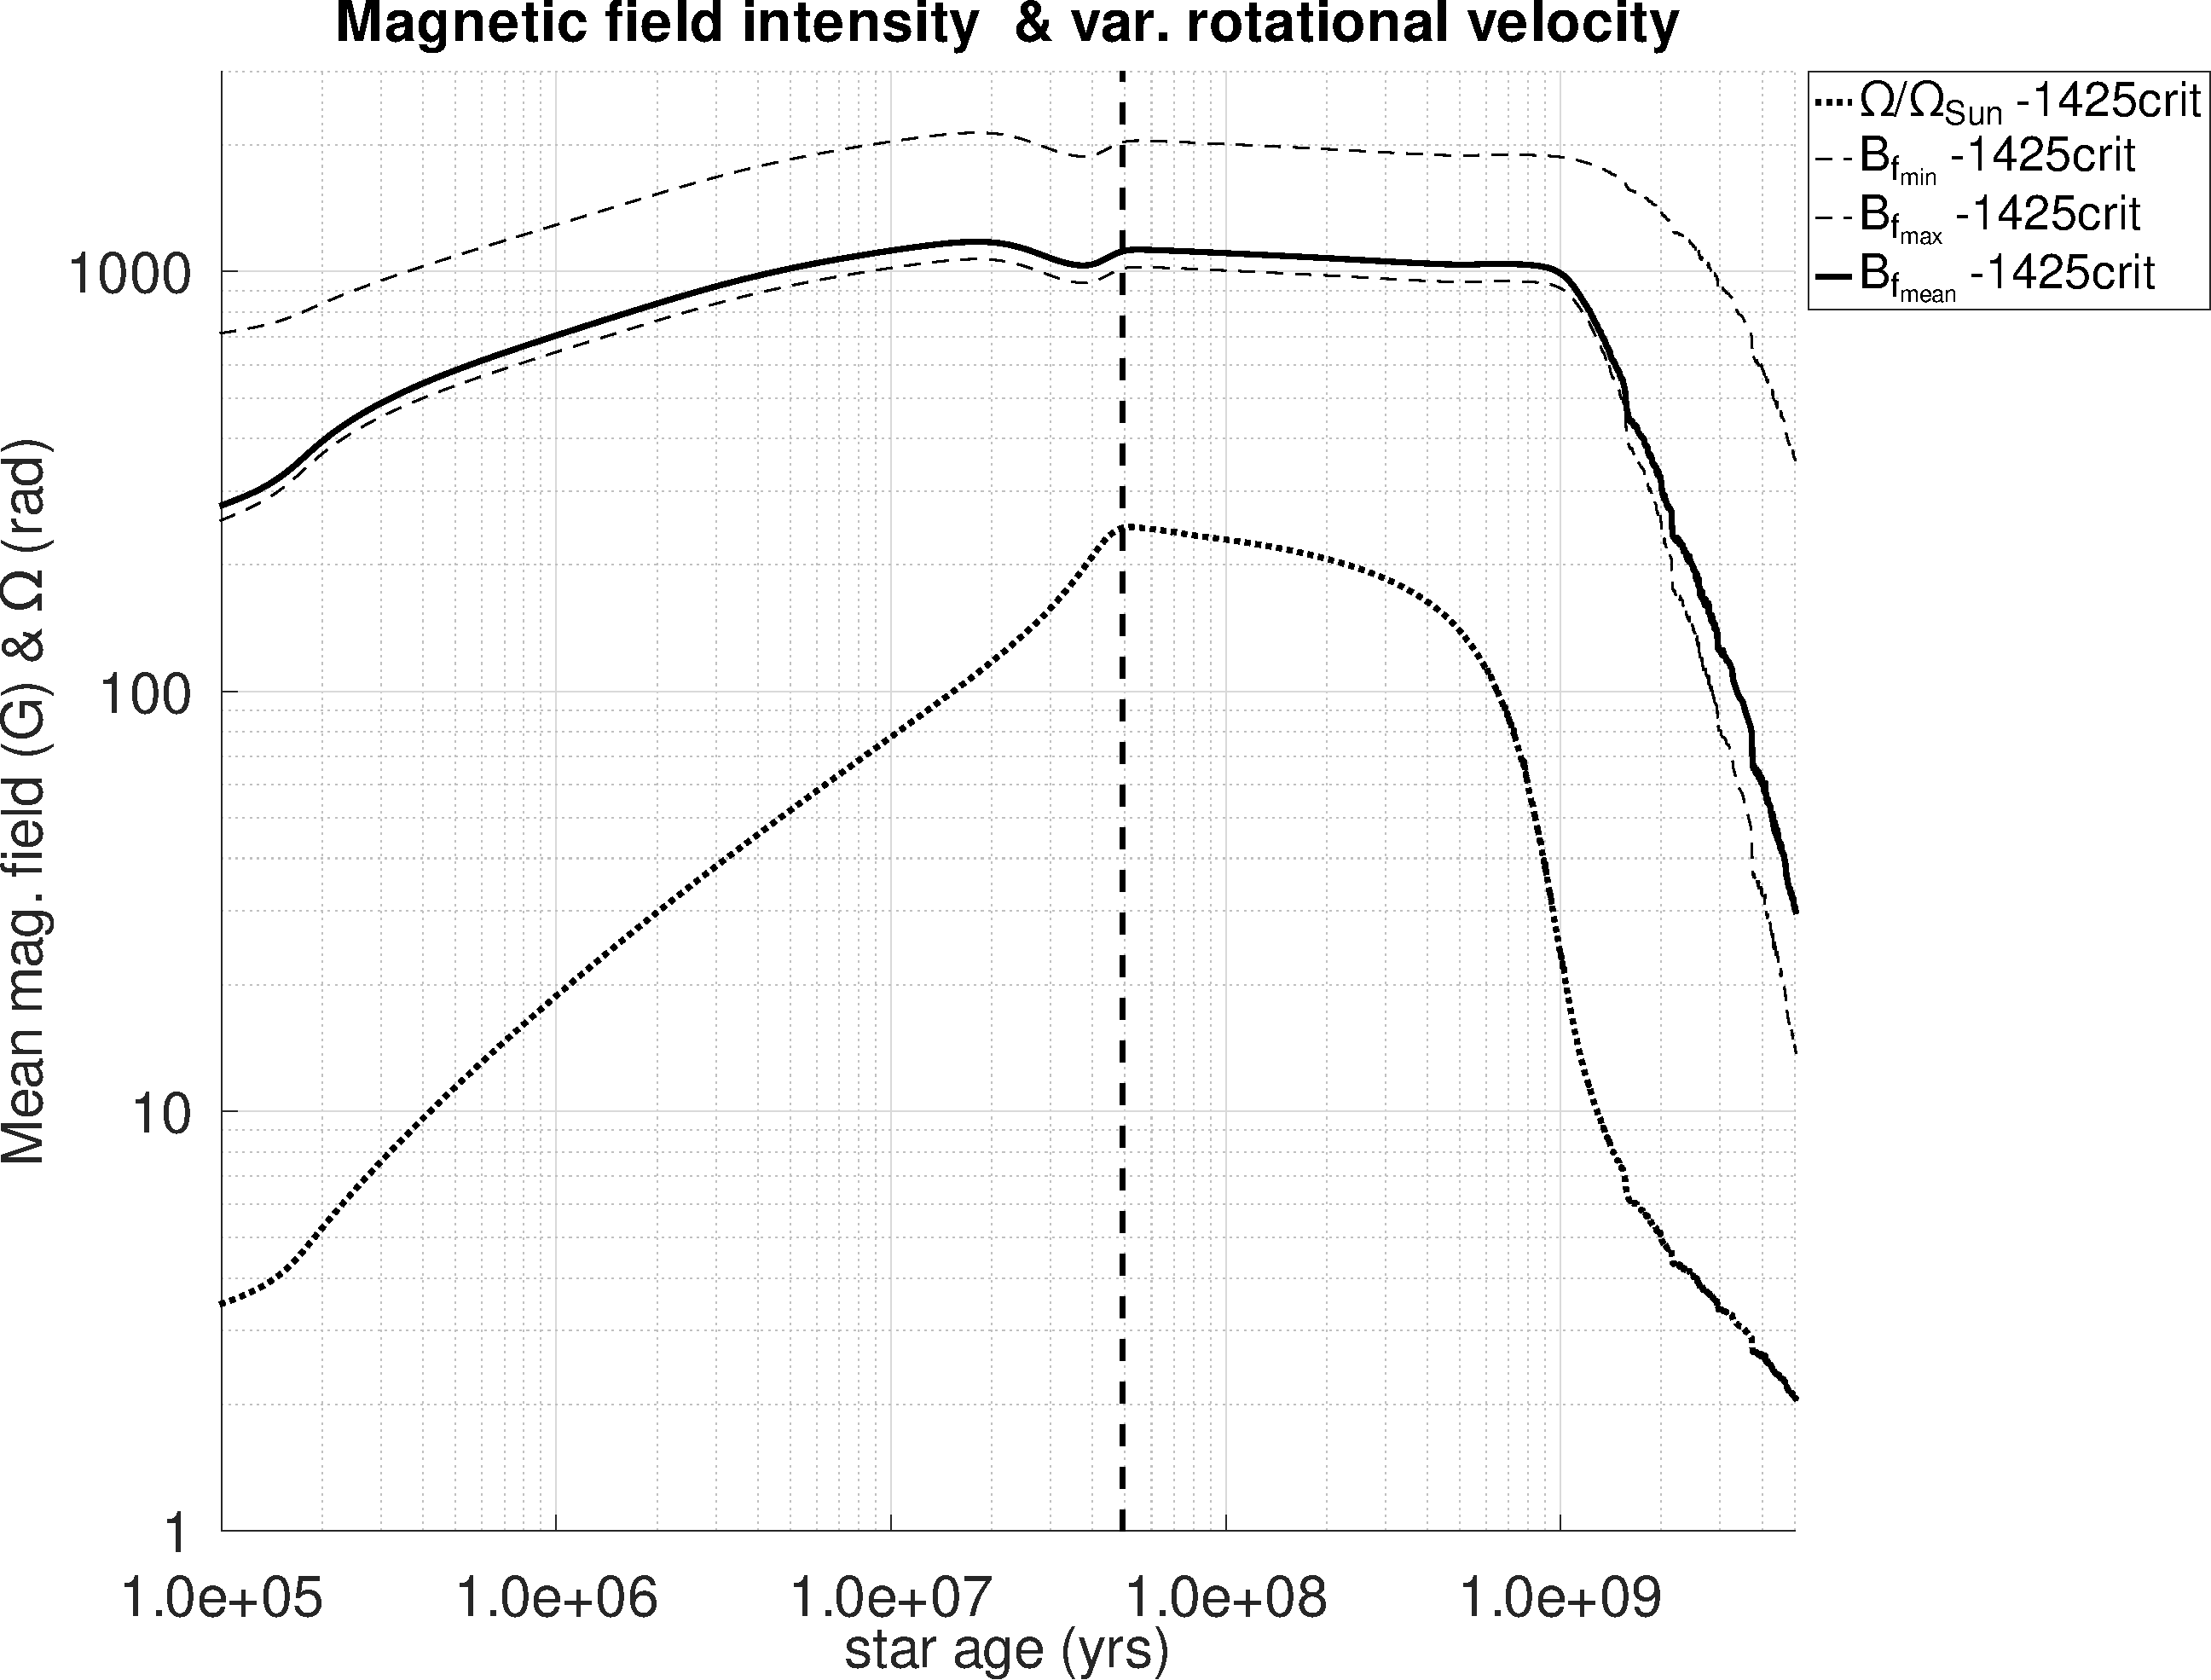
\includegraphics[clip,width=\columnwidth]{figures/paper2/mag_field_limits_var_vel_g3.pdf}
    \caption{The evolution of magnetic field intensity and its upper and lower limits, as a function of time and $\oomegac$ for several 1 $\msun$ models and their. The model include PMS rotation with $\oomegac$ = 0.1425. The solid lines represent the magnetic field strength, while the dotted lines represent the angular evolution of the star. The dashed vertical line makes reference to the ZAMS.}
    \label{fig:mag_field_limits_var_vel_g3}
\end{figure}

With this formalism we are able to calculate the mean magnetic field as a time-dependent function of $\rho$, $\teff$, and $\Omega$. The time values for these three variables will be obtained from the different simulations carried out with the help of MESA.

\subsection{Modelling magnetic braking} \label{mod_mb}
Once we have characterised how the magnetic field strength evolves, we need to model how the loss of angular momentum occurs.  In \cite{Navarro2020} we use a model applicable to magnetic fields of non-variable intensity and of few Gauss ($1.0\,\Gauss \leq B \leq 10.0\,\Gauss$). As shown in Figure \ref{fig:mag_field_limits_var_vel_g3}, the simulations yield magnetic field values that show maximum intensities of around $1.0K\,\Gauss$, making the use of the model employed previously non viable. \par

Let's start by enumerating the most relevant aspects and assumptions made in modelling the evolution of rotation, magnetic braking and angular momentum. If we assume a spherical outflow, the torque applied by a magnetically-coupled stellar winds $\torquewind$ is dictated by,
\begin{ceqn}
\begin{equation}
    \torquewind \propto \Omega_* \; \mwind \; \ralfven^{2} \label{eq:mb_torque}
\end{equation}
\end{ceqn}
where $\mwind$ is the mass loss rate, and $\ralfven$ the averaged value of the Alfvén radius.\par
Stars with similar initial masses but different mass loss ($\Dot{M}$) ratios will end up evolving very differently. The ionized particles carried by the solar wind not only contribute to the mass loss but also to the loss of kinetic energy that is deposited in the interstellar medium. Given a star with a spherically symmetric wind, $\mwind$ is characterized by the following expression:

\begin{ceqn}
\begin{equation}
    \mwind = 4\upi r^2\rho\nu \label{eq:mass_loss}
\end{equation}
\end{ceqn}
where $r$ is the stellar radius, $\rho$ the mass density, and $\nu$ the stellar wind velocity.

It has been observed that strongly magnetic intermediate-mass stars typically have rotation rates much slower than other stars in their parent population \citep{Mathys2006}. In those stars, the magnetic fields interacts with the mass loss, where the Alfv\'{e}n radius plays an important role. $\ralfven$ is defined as the point in which the magnetic field energy density and the kinetic energy density are balanced. In case that $\ralfven$ is greater than the stellar radius, then the wind flow will have to follow the magnetic field. As a consequence, the material leaves the stellar surface with a higher specific AM, as the co-rotation radius has increased and it roughly corresponds to $\ralfven$ which can be expressed as \citep{Matt2012}
\begin{ceqn}
\begin{equation}
    \ralfven = K_1\left[\frac{\Bp^{2}\;R_*^{2}}{\mwind\;\sqrt{K_2^2\vesc^2 + \Omega_*^2R_*^{2}}\ }\right]^{m}R_*  \label{eq:mb_ralfven}
\end{equation}
\end{ceqn}
where $\Bp$ is the magnetic field intensity at the stellar surface, $\vesc$ is the escape velocity, $m = 0.1675$, $K_1 = 1.30$, and $K_2 = 0.0506$ \citep{Gallet2013}.
\begin{ceqn}
\begin{equation}
\vesc = \sqrt{\frac{2\,G\,\mstar}{\rstar}} \label{eq:vesc}
\end{equation}
\end{ceqn}

Finally, we have that the AML can be calculated as follows:
\begin{ceqn}
\begin{equation}
 \Dot{J} = \Omega_* \; \mwind \; \ralfven^{2} \label{eq:j_dot}
\end{equation}
\end{ceqn}
where $\mwind$ is the mass loss rate. This expression is implemented in MESA based on values directly exposed during the simulations.

\subsection{Modelling MLT $\alpha$} \label{mod_mltalpha}
The mixing-length theory (MLT) introduced by Böhm-Vitense (BV) has been commonly adopted to model stellar convection in stellar evolutionary codes, including MESA. The most important free parameter in this theory is the mixing length $l$ which is defined as 
\begin{ceqn}
\begin{equation}
 l = \alpha H_p\label{eq:mixlength}
\end{equation}
\end{ceqn}
where $H_p$ is the pressure scale height, and $\alpha$ a free parameter which is determined in advance and keep fixed during the stellar evolution simulations.\par

 It became evident that the influence of the free, relatively arbitrary, parameters associated with MLT significantly conditioned the evolution of the Li abundance. Moreover, there is no strong arguments which suggest that the mixing-length parameter is the same in all stars and at all evolutionary phases \citep{Pasetto2014}. In \cite{Navarro2020} we showed how an alternative MLT parameterization could produce results in line with the observations. Adjustment of MLT over-shooting and $\amlt$ free parameter seems to be required for explaining Li abundances in OC's.\par

In \cite{Sonoi2018}, the authors introduced a way for calibrating $\amlt$ for solar-like stars in which its value increases with increasing $\gsurf$ or decreasing $\teff$,

\begin{ceqn}
\begin{equation}
 f(x,y) = a_0 + (a_1 + (a_3 + a_5x +a_6y)x + a_4y)x + a_2y\label{eq:alpha_ml}
\end{equation}
\end{ceqn}
where
\begin{ceqn}
\begin{align}
     x &= \frac{\teff-5777}{1000} \label{eq:eq:alpha_x}\\
     y &= \gsurf-4.44 \label{eq:eq:alpha_y}
\end{align}
\end{ceqn}
and $a_i$ are the resulting coefficients of the fitting function \ref{eq:alpha_ml} to the calibrated $\alpha$ values for the MLT-BV convection model \citep{Sonoi2018}: $a_0=1.790295$, $a_1=-0.14954$, $a_2=0.069574$, $a_3=-0.00829$, $a_4=0.013165$, $a_5=0.080333$, $a_6=-0.03306$.\par

\section{Results} \label{sec_3}

\subsection{Grid Models} \label{sec_grid}
In the current work we have replaced two pre-set parameters (alpha and intensity) for the different simulations of our model. Not only have we eliminated the need to assign a value to them, but we allow their values to vary as the simulations evolve over time. The single free parameter of our implementation is $\Omega$. The numerical simulations traced the rotational history and $A(\isotope[7]{Li})$ of a $1\, \msun$ star for a variety of initial values for $\Omega$ (see also Table \ref{tab:phy_mesa}).\par

\begin{table}
	\centering
	\caption{Summary of adopted physics in MESA \citep[based on][]{Choi2016,Navarro2020}.}
	\label{tab:phy_mesa}
	\begin{tabular}{ll} 
		\hline
		Parameter & Adopted prescriptions and values\\
		\hline
		Solar Abundance & $X_{\odot}=0.7154, Y_{\odot}=0.2703, Z_{\odot}=0.0142$\\
		Equation of State & OPAL+SCVH+MacDonald+HELM+PC\\
		Opacity & OPAL Type I for log T $\geq$ 4 \\ & Ferguson for logT $\leq$ 4\\
		Reaction Rates & JINA REACLIB\\
		Boundary Conditions & ATLAS12; $\tau$=100 tables + photosphere\\
		Diffusion & Track \isotope[1]{H}, \isotope[2]{He}, \isotope[7]{Li}, \isotope[7]{Be}\\
		Rotation & Differential rotation at PMS \& MS\\
		Convection & MLT + Ledoux, variable $\alpha_{{\rm MLT}}$\\
		Overshoot deactivated & $f_{{\rm ov,core}}=0.0$, \& $f_{{\rm ov,sh}}=0.0$\\
		Semiconvection & $\alpha_{{\rm sc}}=0.1$\\
		Thermohaline & $\alpha_{{\rm th}}=666$\\
		Rotational Mixing & Include SH, ES, GSF, SSI \& DSI\\
            Mixing Length Theory & $\alpha_{{\rm MLT}}$ variable depending on $\teff$\\ & \& $\gsurf$\\
		Magnetic Effects & Magnetic braking based on idealized \\ & dipole field\\
		Magnetic Field & B(G) variable, depending on $\rho$, $\teff$ \&  $\Omega$\\\
		Mass Loss & activated, $\Dot{M}_{{\rm max}} = 10^{-3} \: \msun \: yr^{-1}$\\
		Angular Moment Loss & activated, $\Dot{J} = \Omega_* \; \mwind \; \ralfven^2$\\
		\hline
	\end{tabular}
\end{table}

Most of the configuration used in the simulations remain the same as in our previous work, with the exception of the overshooting (deactivated), the $\amlt$ pre-set value, and the formalism used for calculating $\Dot{J}$ (see \cite{Navarro2020} for further details).\par

The models continue to including rotation during the PMS. We adopted a simple and pragmatic theoretical approach to establish when the star is reaching the ZAMS phase: the simultaneous existence of an extensive convective layer and a radiative core. From this moment on, the MB routine was activated, acting as an additional mechanism to those existing in the MESA evolutionary code that participated in the star AML. This time, the restriction of a magnetic field with a constant intensity throughout the evolution of the star until it reached the TAMS is removed in favor of variable one. Something similar happens with $\amlt$ which indeed is  a key factor to determine the near-surface structure of stellar models. 

In this new paper we continue to focusing on the indirect role played by the MB on the Li destruction. The main objective continues to be to check how MB could contribute to explain the evolution of Li in the Sun and other solar-type stars. We computed the evolution of $1\,\msun$ stellar models at solar initial metallicity with $\oomegac$ varying between $0.12$ and $0.1425$. The results are then compared with the data collected by the Gaia mission and GES for the stars belonging to the OC's referenced in Table \ref{tab:oc_list}.\par


As expressed by Eq.~\ref{eq:mb_torque}, the amount of AML depends on $\ralfven$, $\Omega$ and $\Dot{M}$. For large $\ralfven$ values, the star undergoes a significant deceleration. The value of $\ralfven$ depends on the following varying parameters: magnetic field ($B$) intensity, $\teff$ and$\Omega$. With regards to $\Dot{M}$ and as reported in Table \ref{tab:phy_mesa}, the empirical formula developed by Reimers \citep{Reimers1975} for stars in the asymptotic giant branch (AGB) was used for calculating the mass-loss. For a solar-type star the $\Dot{M}$ during MS is relatively small, about  $10^{-14}\msun \, yr^{-1}$ \citep{Noerdlinger2008}. \par

MESA assigns an $\Omega$ value for each cell $k$ ($\Omega_k$) which is adjusted so that the resulting angular momentum is retained after calculating the new mass of the cell $k$ ($m_k$) and its distance to the center of the star ($r_k$). After that, an AM value is assigned to each cell $k$ ($J_k$). At this point, our MB turns on, modifying $J_k$. This was done by providing an additional contribution ($\Dot{J}_{k}$). This contribution is the result of the external torque exerted by the magnetic field once it has been distributed among the different layers that make up the CZ as dictated by Eq.~\ref{eq:k_jdot}:\par
 
\begin{ceqn}
\begin{align}
    \Dot{J}_{k} &= \Dot{J}_*\;\frac{m^{}_{k} r^2_{k}}{m^{}_* r_*^2} \label{eq:k_jdot}
\end{align}
\end{ceqn}

\subsection{Li evolution with MB}
Figure \ref{fig:li_var_vel_var_g_3} shows the temporal evolution of surface Li abundance for several 1 $\msun$ models. Those models were initialized with different rotational velocities and took into consideration the effects of MB caused by a variable magnetic field which its intensity evolution is shown in Figure \ref{fig:mag_field_var_vel_g3}. If we compare it with Figure \ref{fig:li_var_vel_0g} in which the effects of MB were neglected, we notice how the profiles of Li abundance were altered during PMS and MS. During the PMS we can describe the effect as modest, somewhat expected and in line with the fact that the AML caused by MB (see Eq.~\ref{eq:j_dot}) depends directly on the mass loss rate (see Figure \ref{fig:mdot_var_vel_g3}) and the $\Omega$ (see Figure \ref{fig:rot_vel_var_vel_var_g3}) evolution. If we take into account that for solar-type stars the models predict a modest total mass loss rate, that value is even much lower in this phase. It is in the approach phase to the TAMS that the angular velocity reaches its maximum. This, according to our model, plays a crucial role in both the mass loss and the magnetic field strength. The higher the $\Omega$, the higher the $\Dot{M}$, and therefore the higher the magnetic field strength. These effects combine and lead to an accentuation of the magnetic braking effect. As a consequence, there is a slowing down of Li destruction once the models enter the MS. The results of our simulations for those models respectively initialized to $\oomegac$ = 0.14 and 0.1425 reproduce A(Li) in line with that of the Sun surface \isotope[7]{Li} abundance  (1.1 $\pm$ 0.1 dex). The latter gives a value of 1.133 dex, which would represent a deviation of about 3\% from the nominal value.\par

\begin{figure}
	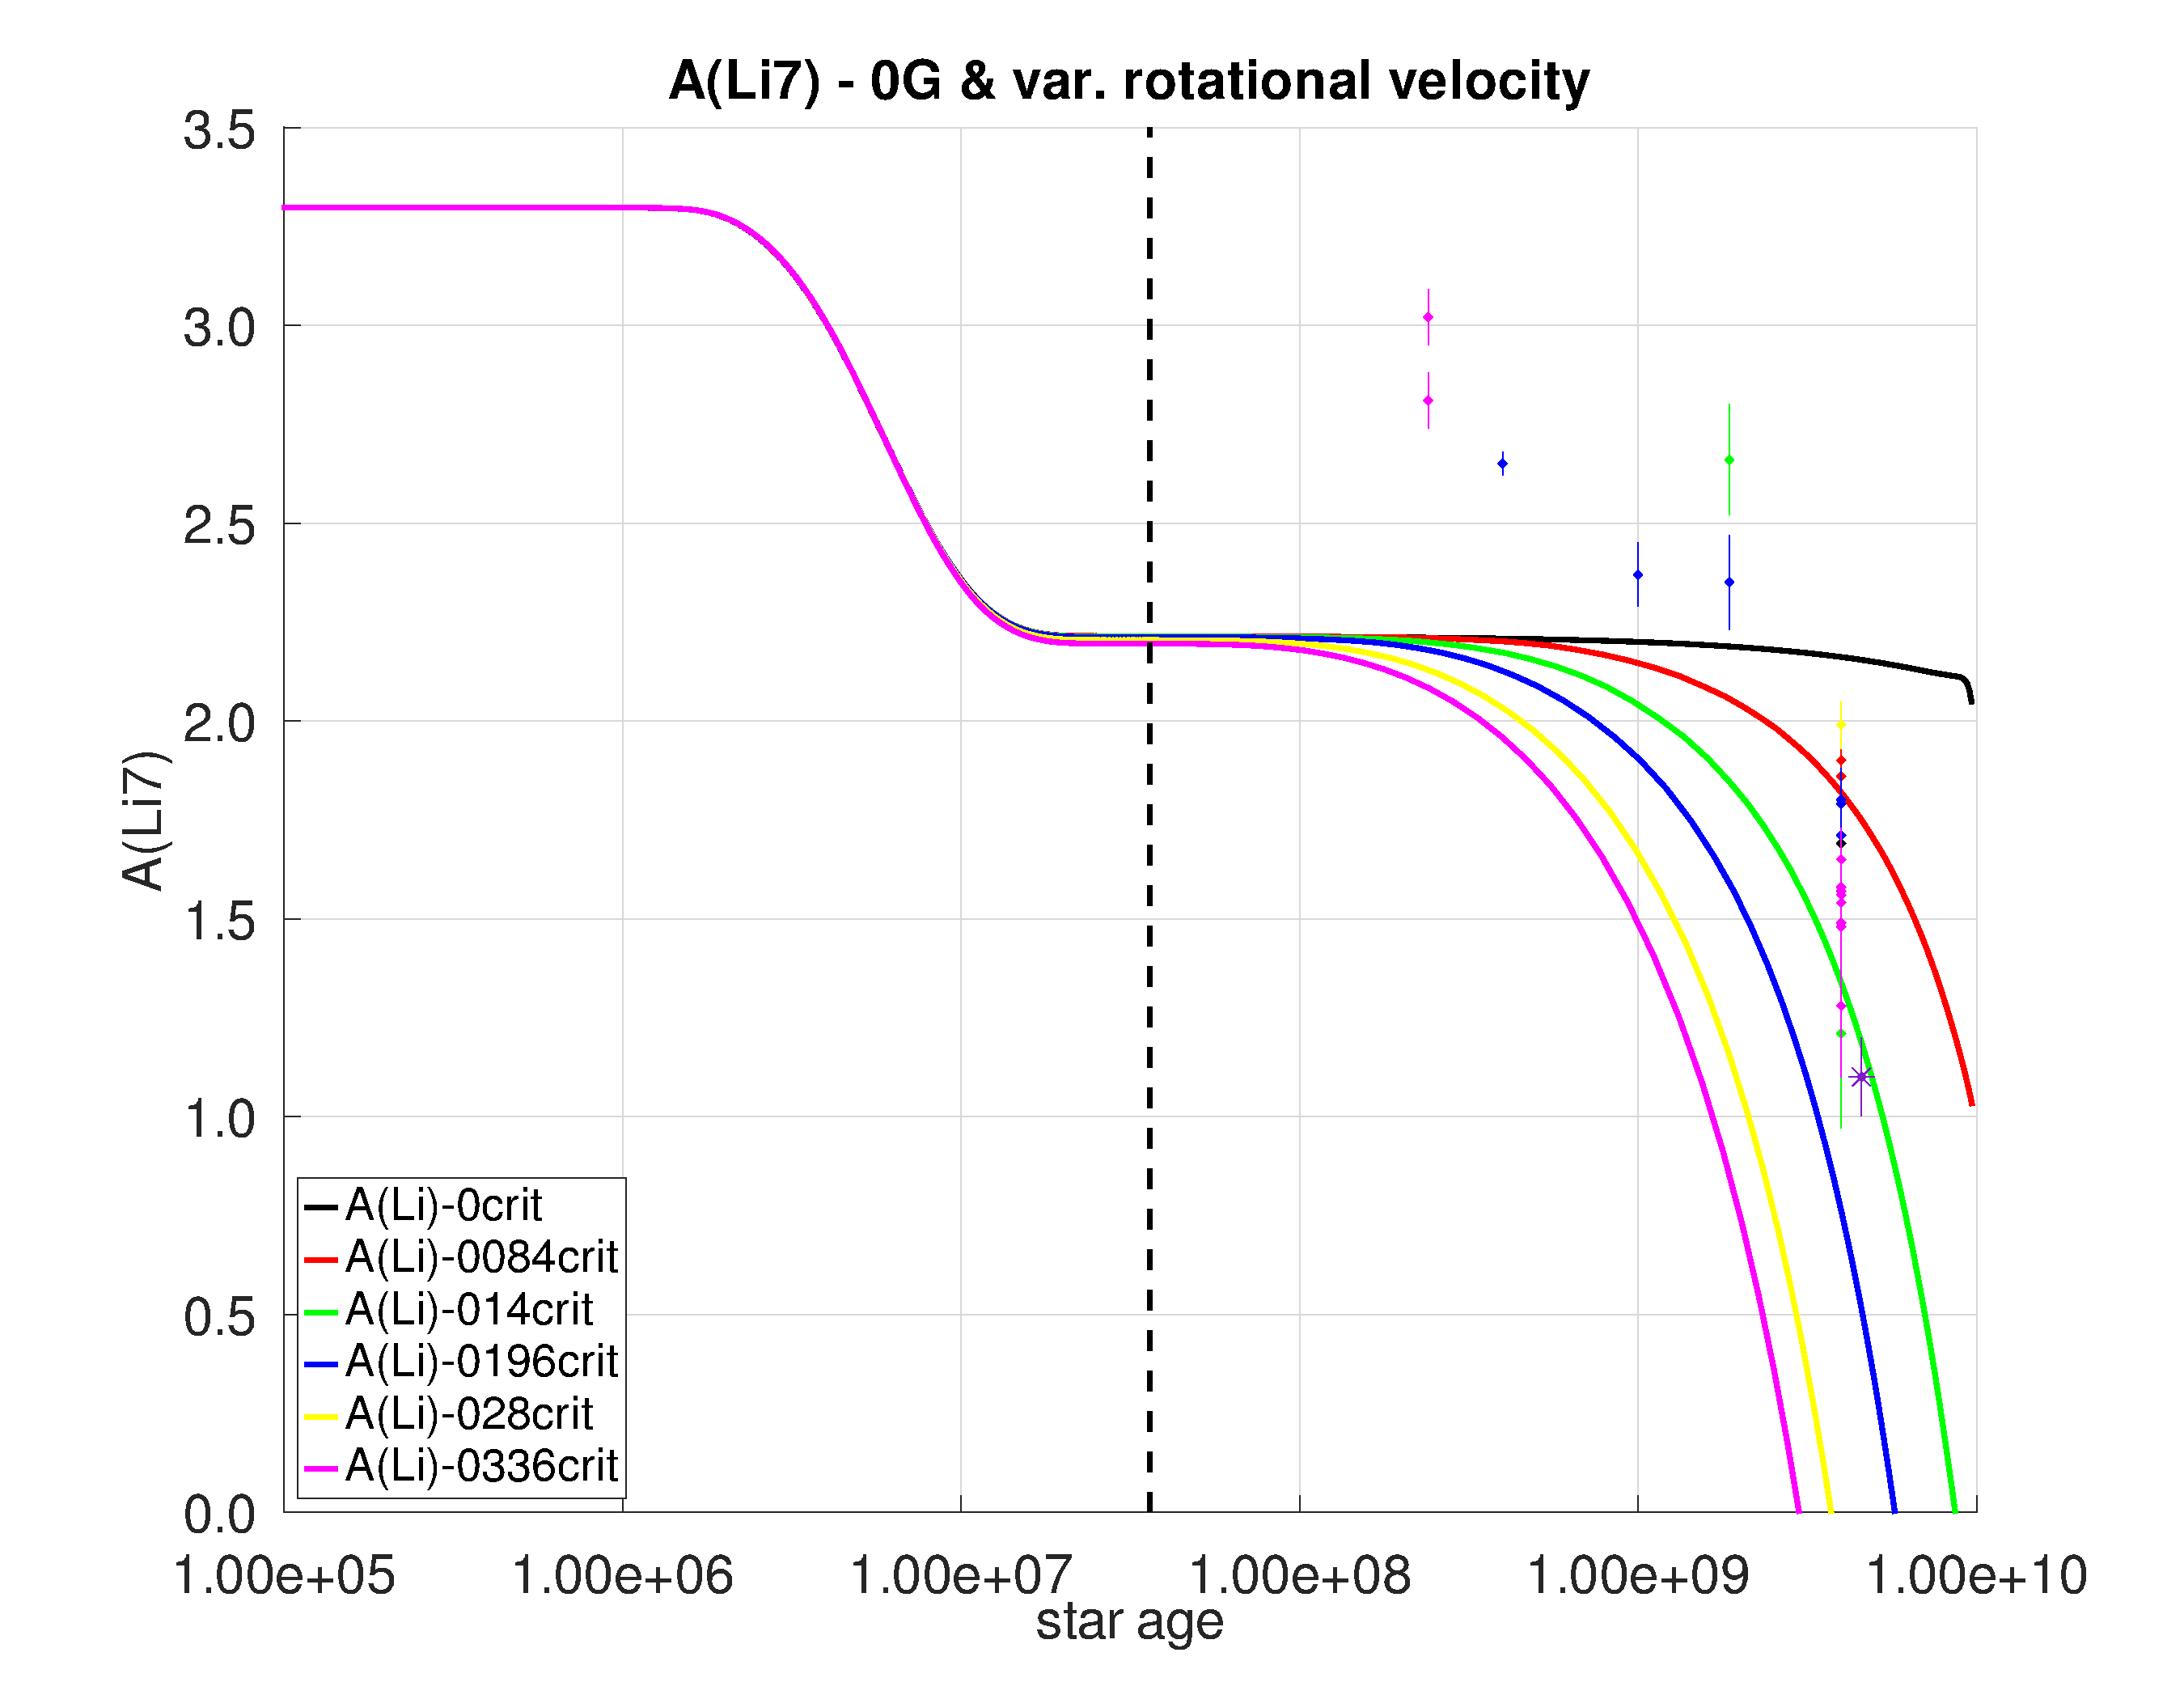
\includegraphics[trim = 25mm 10mm 15mm 10mm, clip, width=\columnwidth]{figures/paper2/li_var_vel_0_0g_0.pdf}
    \caption{The evolution of surface \isotope[7]{Li} abundance relative to \isotope[1]{H}, as a function of time for several 1 $\msun$ models. The solid black line represents the reference model according to \citet{Choi2016}. The rest of lines are models which include PMS rotation with $\oomegac$ between 0.0084 and 0.0336, respectively. The purple star and square are surface Li abundances for the present-day Sun \citep{Asplund2009} and the average for the Pleiades cluster \citep{Sestito2005} respectively. The dashed vertical line makes reference to the ZAMS. (Figure taken from \citet{Navarro2020}.)}
    \label{fig:li_var_vel_0g}
\end{figure}

\begin{figure}
	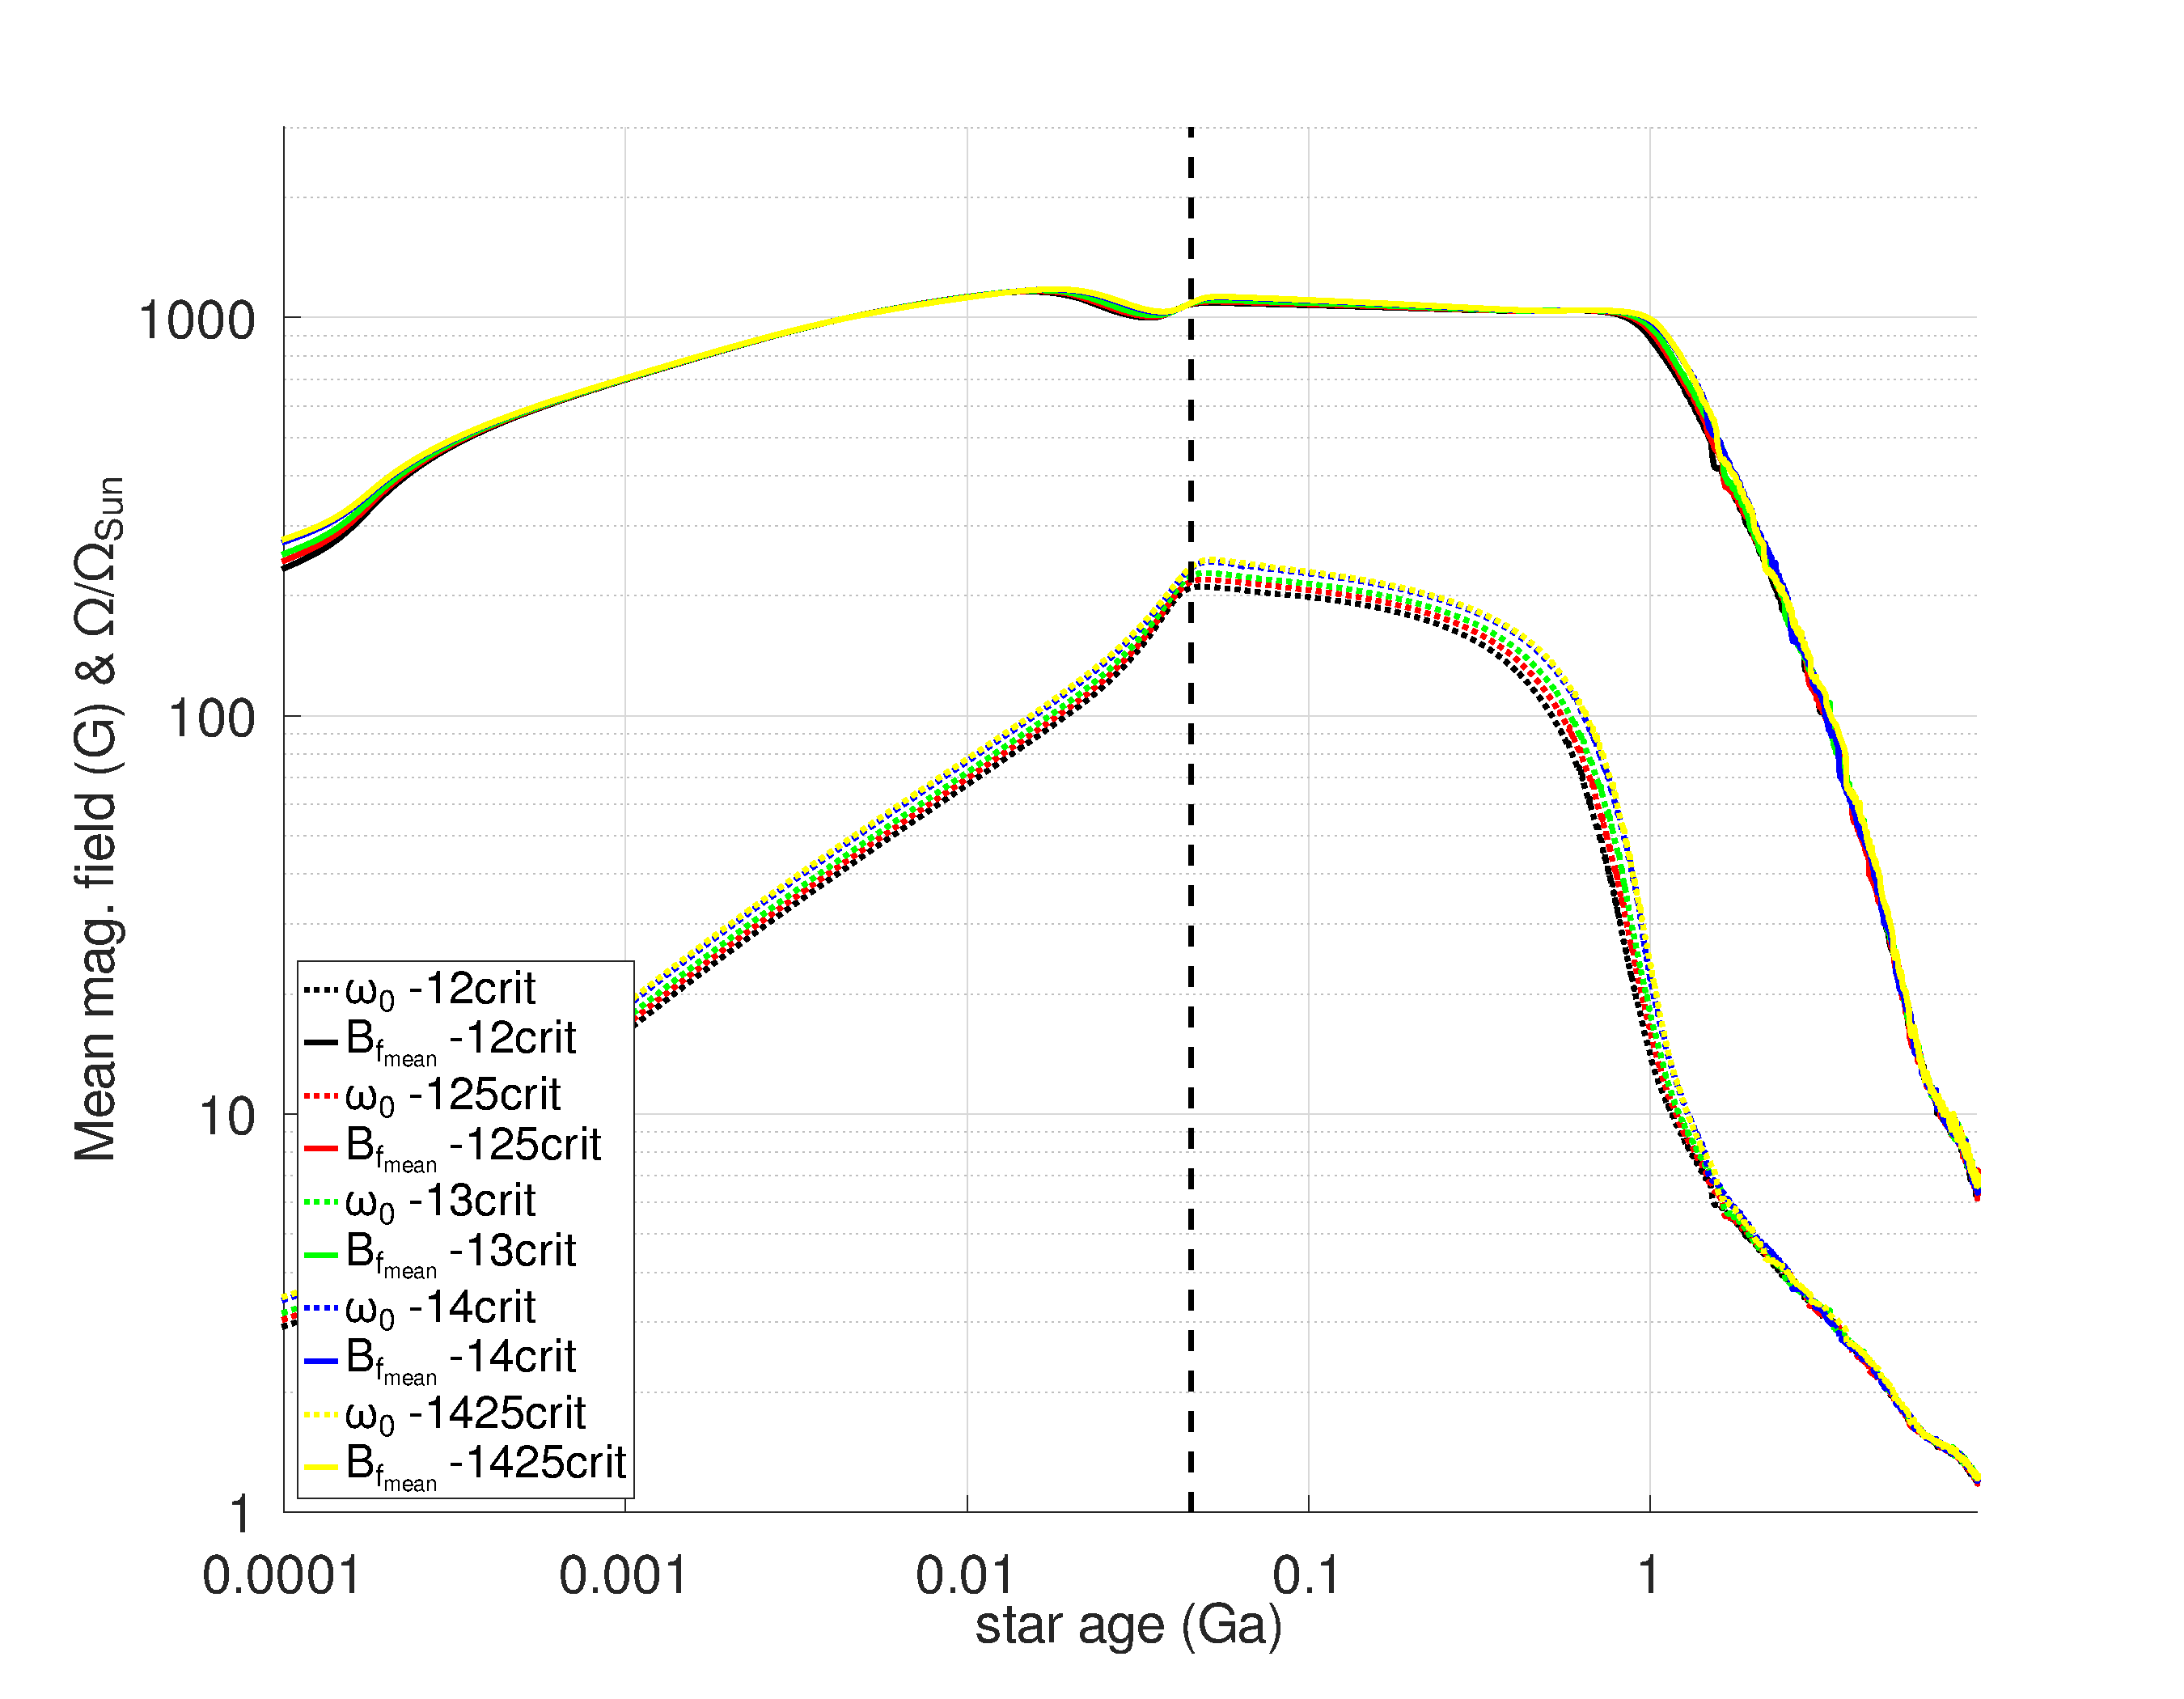
\includegraphics[clip,width=\columnwidth]{figures/paper2/mag_field_var_vel_g3.pdf}
    \caption{The evolution of magnetic field intensity, as a function of time and $\oomegac$ for several 1 $\msun$ models and their. The models include PMS rotation with $\oomegac$ between 0.12 and 0.1425. The solid lines represent the magnetic field strength, while the dotted lines represent the angular evolution of the star. The dashed vertical line makes reference to the ZAMS.}
    \label{fig:mag_field_var_vel_g3}
\end{figure}

In Figure \ref{fig:rot_vel_var_vel_var_g3} we depict the rotation profiles for the surface of the stars and for the bottom of the convective envelop. It shows how the angular velocity increases in value as the star decreases in radius along the PMS. During this stage of its evolution, the star has a nearly convective structure, as can be seen in Figure \ref{fig:cz_var_vel_var_g3}. As it approaches the ZAMS at $\approx 10^6$ years, the convective zone of the star begins to shrink in size and the core of the star reaches the temperature, pressure and density conditions necessary to develop a radiative core. In turn, the difference in the angular velocities of the different models becomes more evident, being higher in those that were initialised with a higher initial angular velocity. This fact implies that the mass loss is also higher for those stars that rotate faster. As we have described above, a larger mass loss also implies a larger angular momentum loss. The combined effects of the increases in effective temperature, angular velocity and mass loss cause the magnetic field strength to reach its maximum in the approach phase of the ZAMS (see Figure \ref{fig:mag_field_var_vel_g3}). We observed that the models with lower angular velocity generally ended up exhibiting higher values for the Li abundance on the surface (see Figures~ \ref{fig:li_var_vel_var_g_3}, \ref{fig:grid_li_var_vel} \& \ref{fig:grid_li_var_g}). For these same simulated models initialized to $\oomegac$ = 0.14 and 0.1425, the values obtained for the $\Omega$ and the magnetic field strength are far from the measurements obtained for the Sun. $\osun$ is 2km/s with a minimum error of 3m/s, and the mean magnetic field strength is 1G. For the simulation with $\oomegac$=0.1425, we obtain a rotational velocity of 4.72km/s, which represents a 235\% deviation, and for the average magnetic field strength we have 36.9G, far away from the reference value.\par

\begin{figure}
	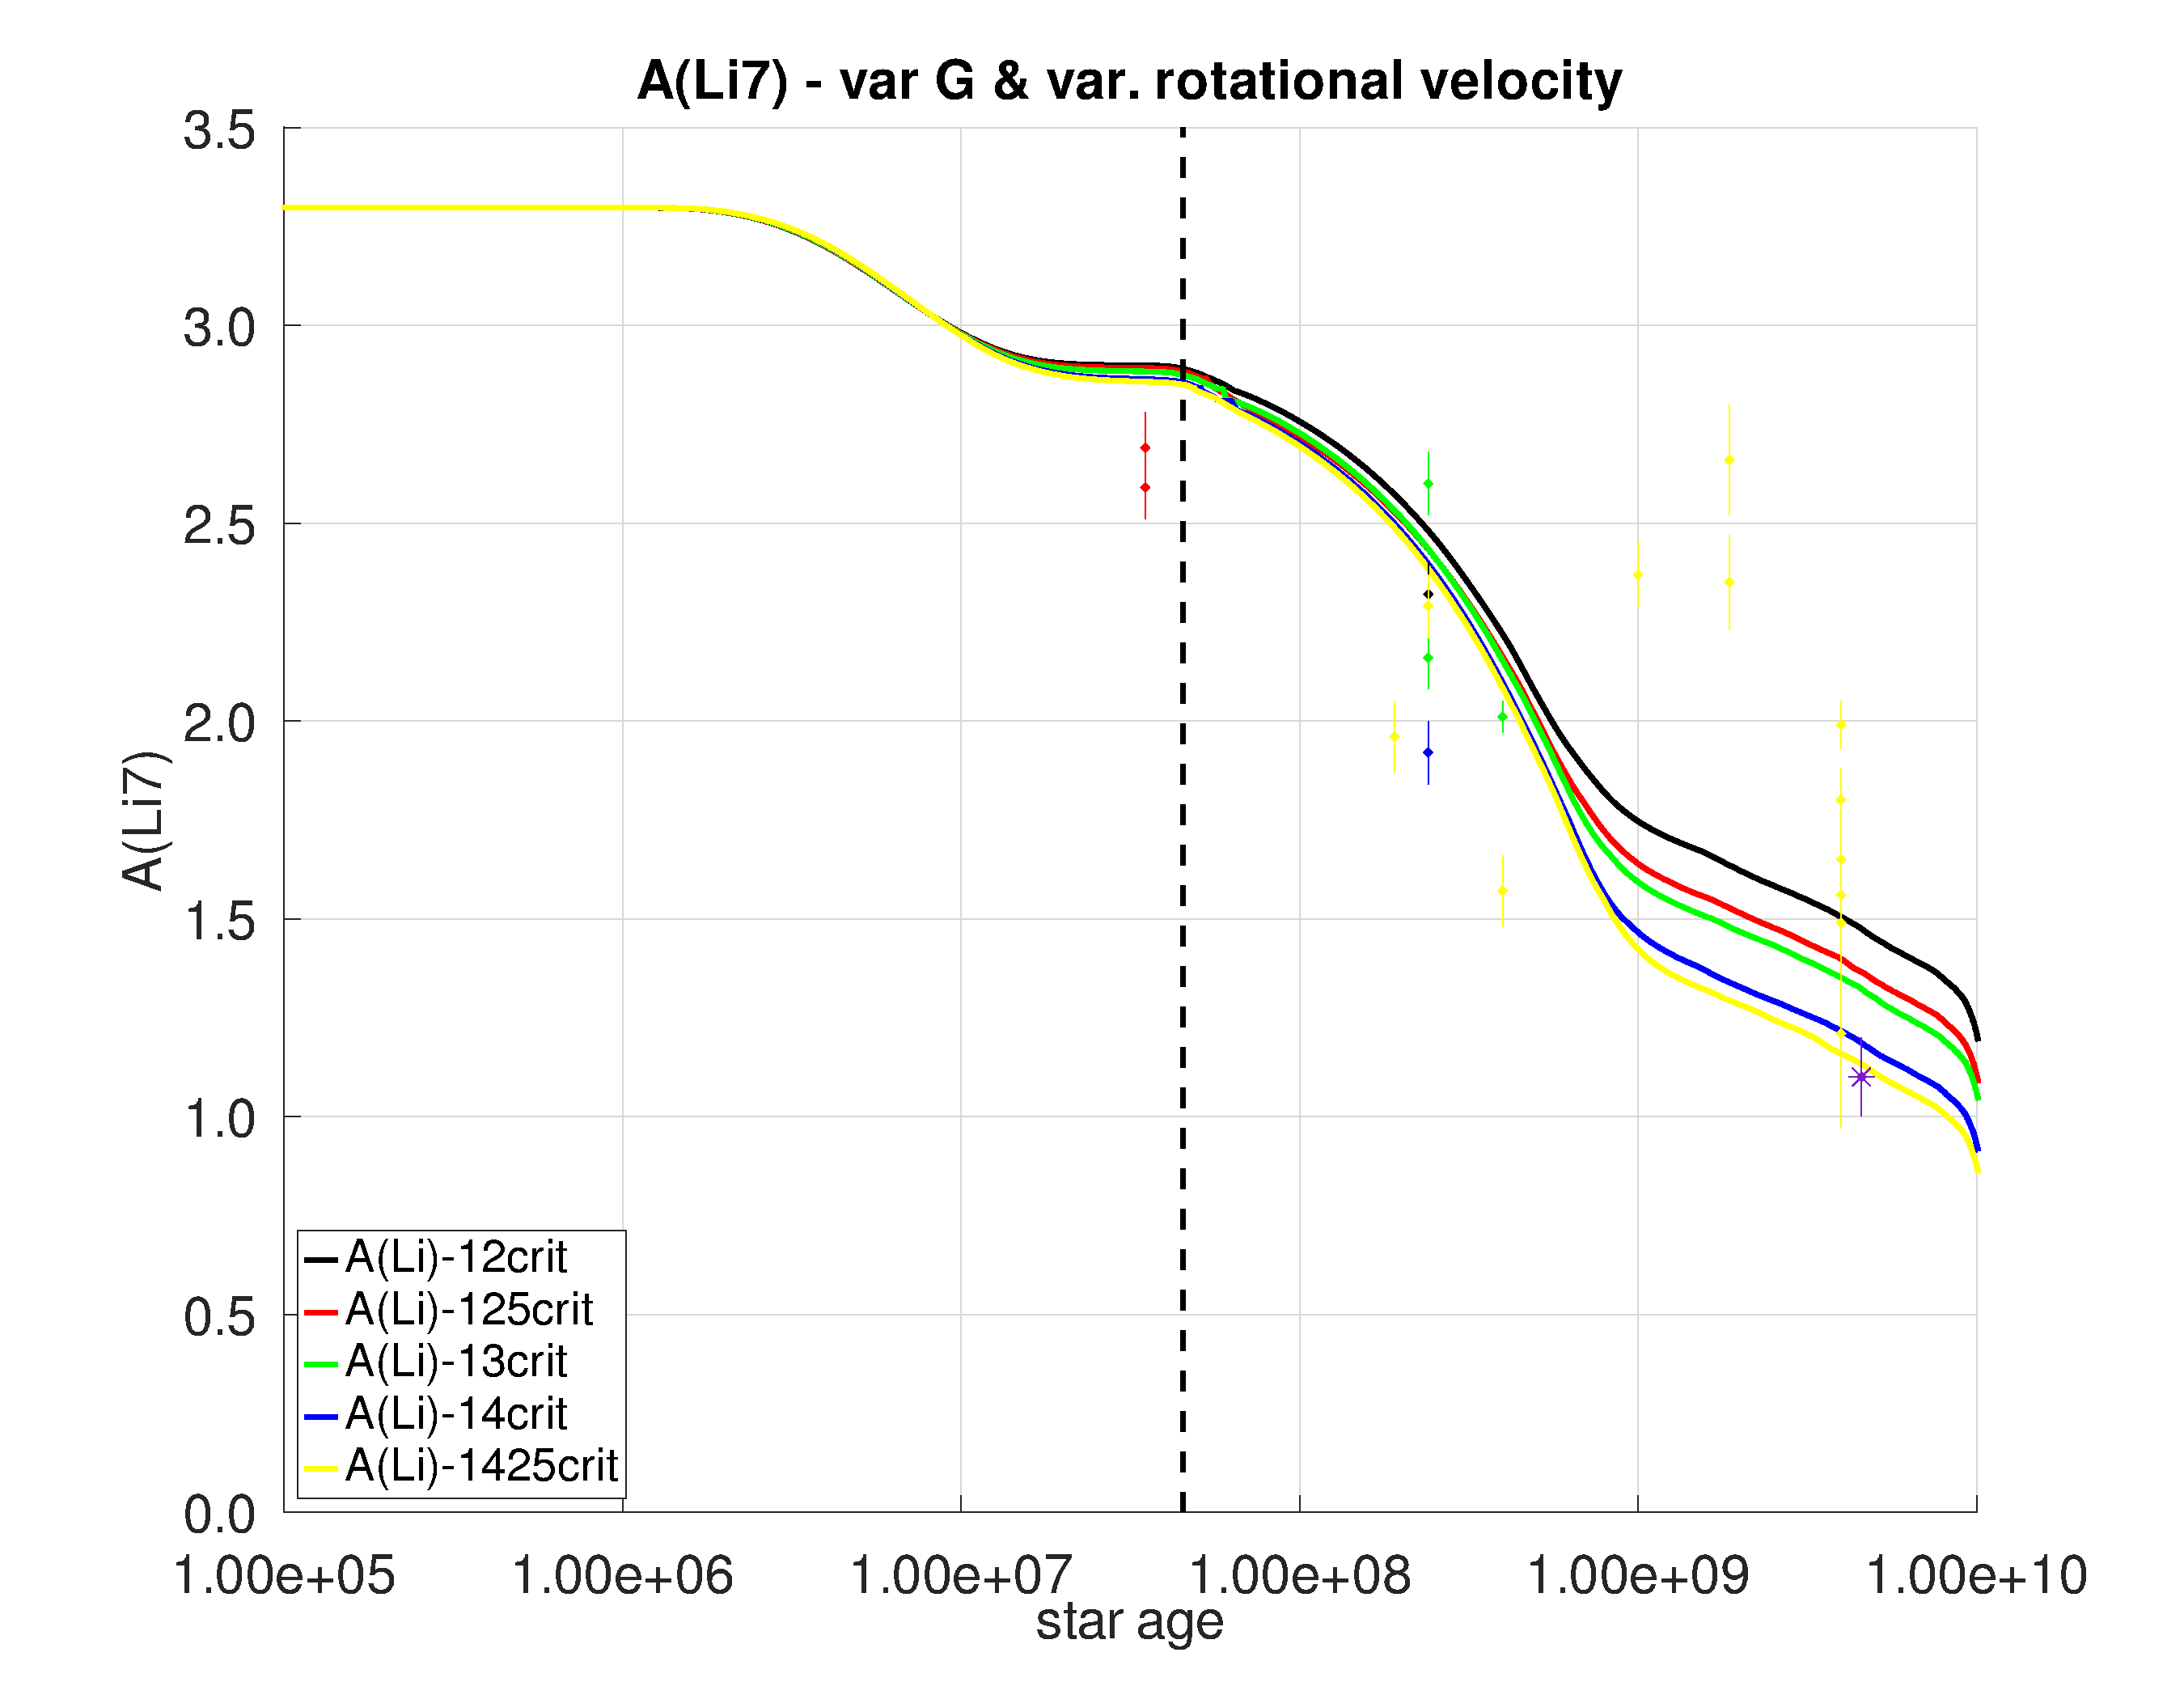
\includegraphics[clip,width=\columnwidth]{figures/paper2/li_var_vel_var_g_3.pdf}
    \caption{The evolution of surface \isotope[7]{Li} abundance relative to \isotope[1]{H}, as a function of time for several 1 $\msun$ models. The models include a magnetic field with variable intensity, PMS rotation with $\oomegac$ between 0.12 and 0.1425, respectively and MB. The purple star is the surface angular velocity for the present-day Sun \citep{Gill2012}. The rest of the dots in different colours represent surface \isotope[7]{Li} abundances of stars with similar parameters to the evolution curve represented with the same colour.The dashed vertical line makes reference to the ZAMS.}
    \label{fig:li_var_vel_var_g_3}
\end{figure}

As described in section \ref{mod_mb}, the MB routine distributed the total amount of AML calculated according to Eq.~\ref{eq:k_jdot} among the different layers that composed the CZ. In Figure \ref{fig:cz_var_vel_var_g3} we can observe the evolution of the most external CZ normalized with respect to the radius of the star for several 1 $\msun$ models. The models include a magnetic field with variable intensity, PMS rotation with $\oomegac$ between 0.12 and 0.1425. In accordance with the established models of stellar evolution, in a solar-type star the CZ covers practically all of it for a large part of the PMS. From the ZAMS on-wards, its size starts to decrease gradually in a first phase and then becomes more pronounced at around $4.0x10^8$ years of age. This change in the size of the CZ is due to magnetic braking. As can be seen in Figure \ref{fig:rot_vel_var_vel_var_g3}, the star, after reaching its maximum angular velocity when passing the ZAMS, starts to decelerate due to magnetic braking. In our models the magnetic braking routine is activated when the star develops a radiative core and the existence of a convective zone above it (see Figure \ref{fig:mb_act_var_vel_g3}). It is the presence of the MB that prevents the star from further increasing its angular velocity. In this way, the Li destruction is attenuated by a lower rotational velocity. The models start to decelerate gradually once the ZAMS is passed and during the initial period of their stay in the MS. The magnetic field strength remains close to its maximum, decreasing slightly and then decreasing more sharply. Its behaviour reflects that of the evolution of the angular velocity, a consequence of the effects of the MB. The deceleration process continues progressively until, around the present age of the Sun, we obtain angular velocity values very similar to the Sun. The deceleration leads to a reduced effect of centrifugal forces, which allows for a contraction of the star's radius, and thus a smaller size of the CZ. Additionally, a lower angular velocity has an effect on the magnetic field strength, as can be seen in Figure \ref{fig:mag_field_var_vel_g3}. The coupling between angular velocity, magnetic field strength, and star radius is evident and consistent.\par

\begin{figure}
	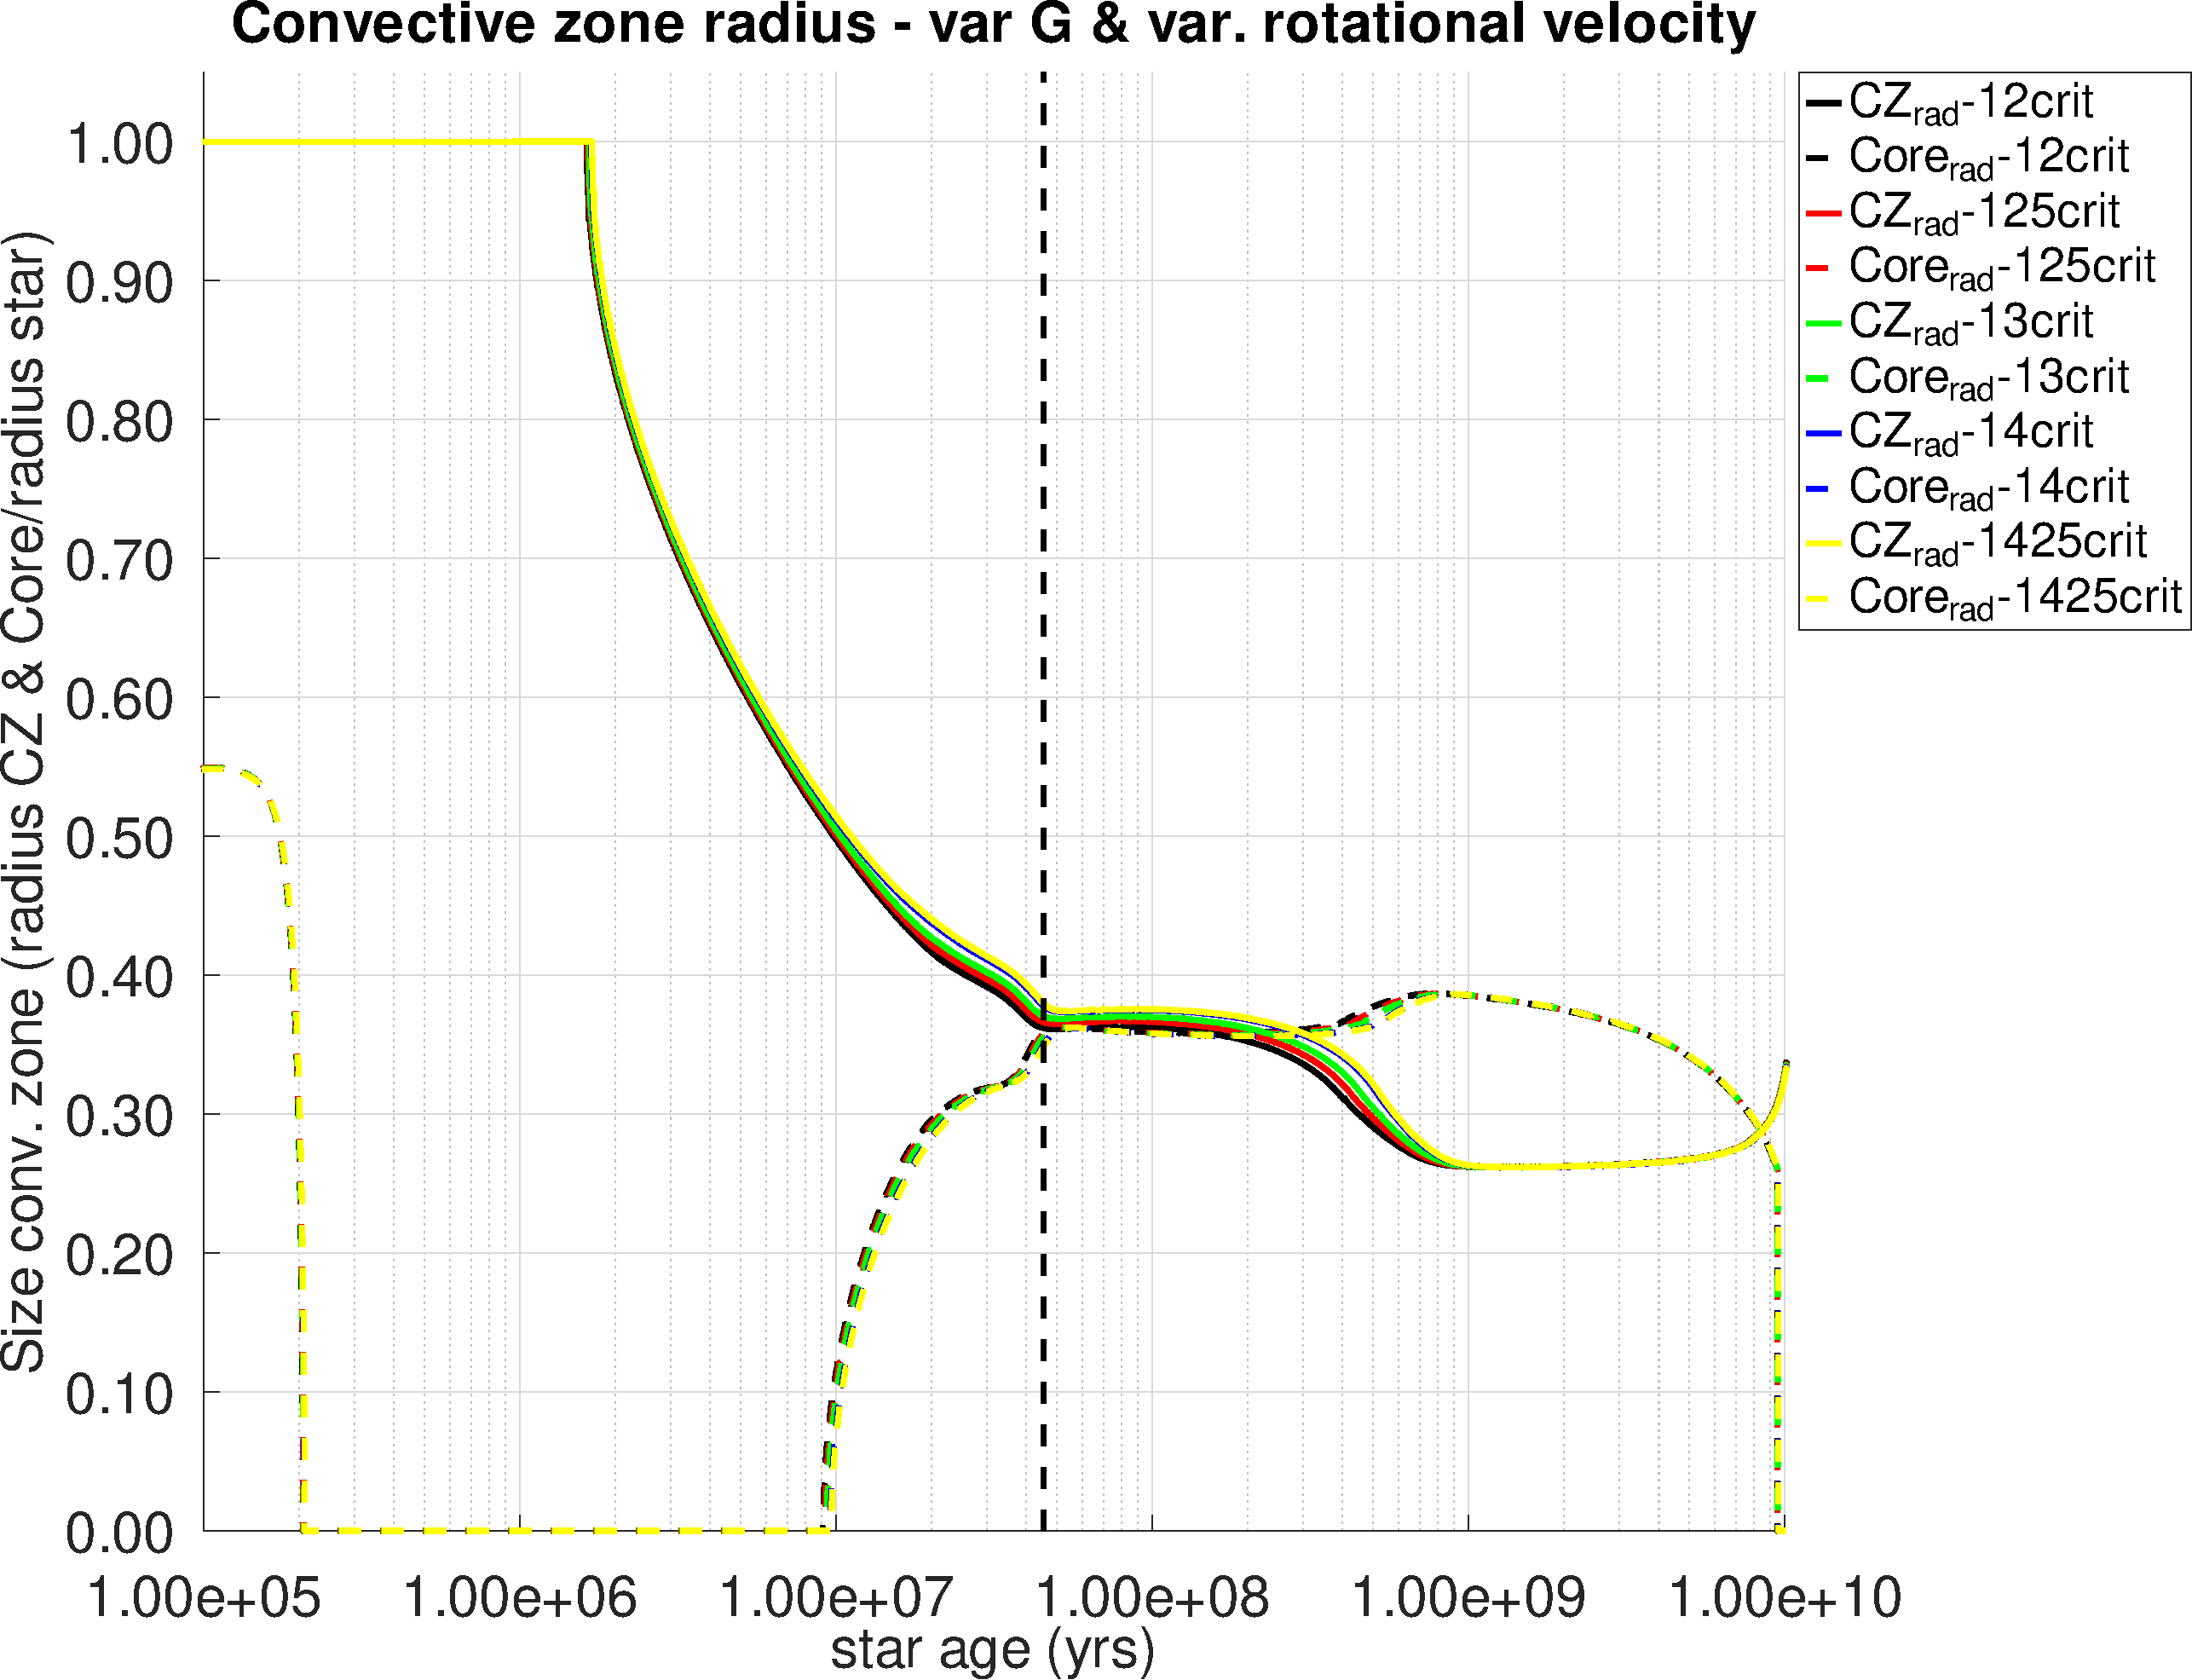
\includegraphics[clip,width=\columnwidth]{figures/paper2/cz_var_vel_var_g3.pdf}
    \caption{The evolution of radiative and convective zones size as a function of time for several 1 $\msun$ models. The models include a magnetic field with variable intensity, PMS rotation with $\oomegac$ between 0.12 and 0.1425. The dashed vertical line makes reference to the ZAMS.}
    \label{fig:cz_var_vel_var_g3}
\end{figure}


\begin{figure}
	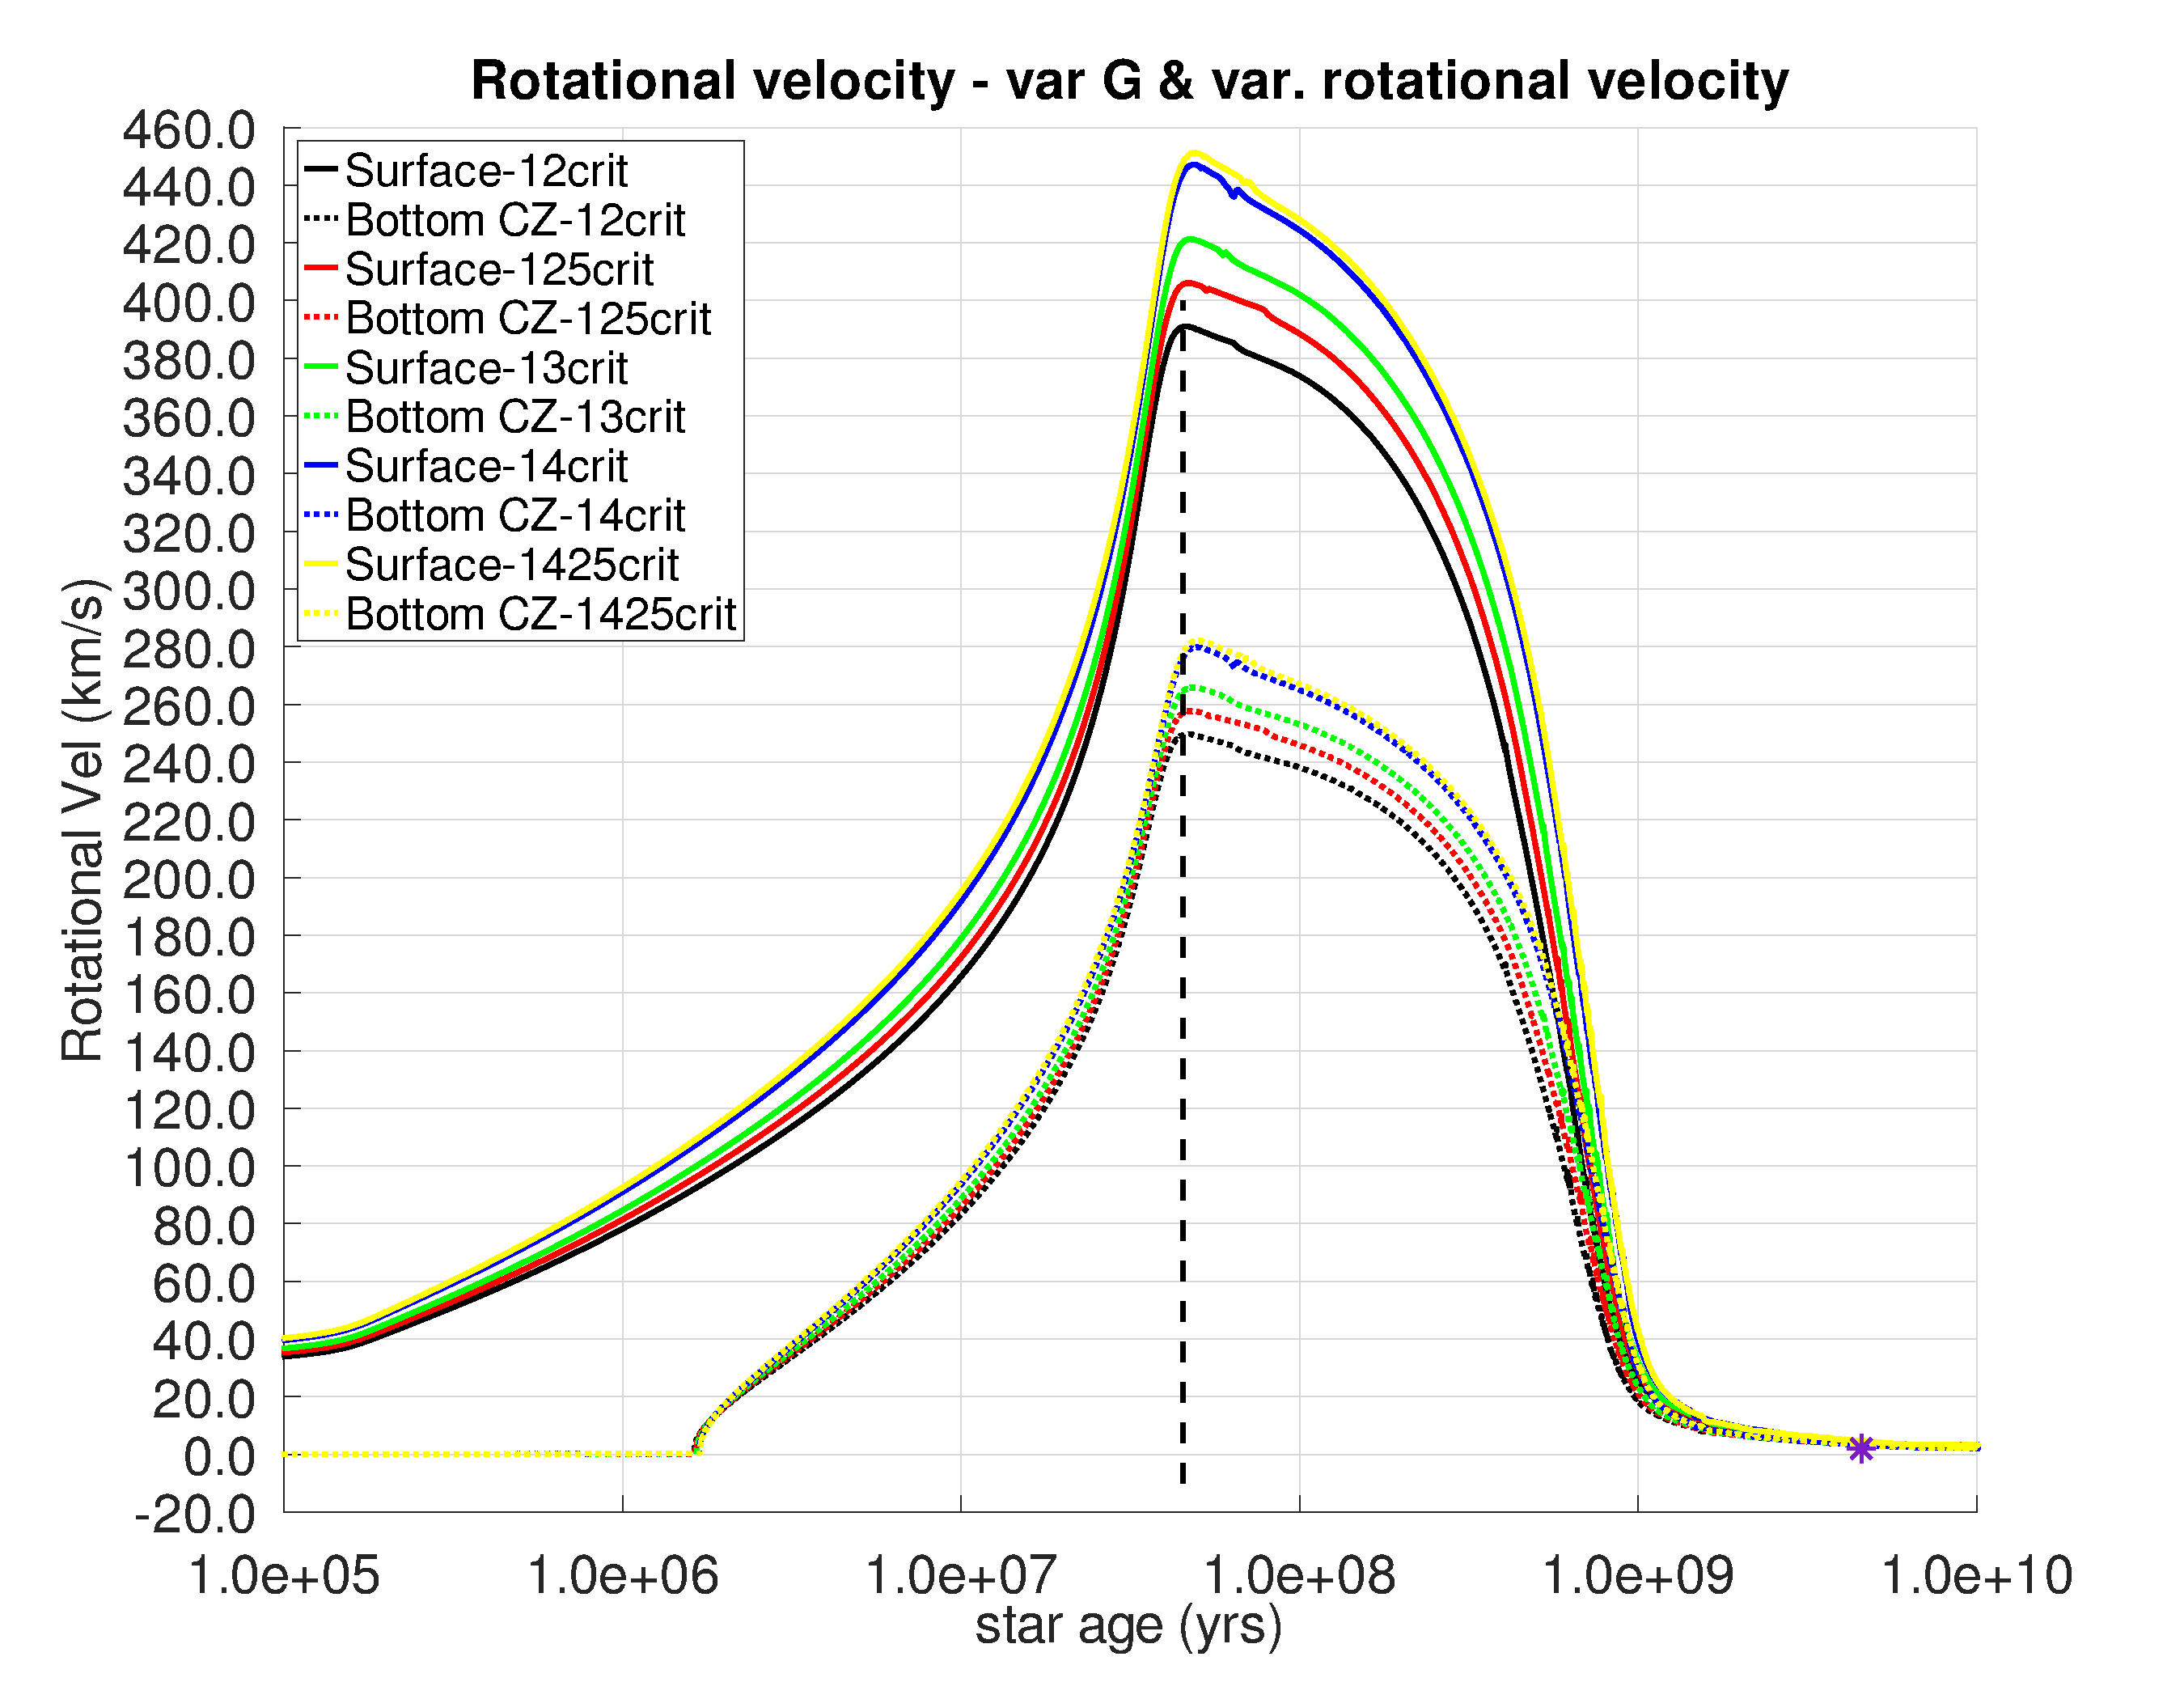
\includegraphics[clip,width=\columnwidth]{figures/paper2/rot_vel_var_vel_var_g3.pdf}
    \caption{The evolution of surface rotational velocity, as a function of time for several 1 $\msun$ models. The models include a magnetic field with variable intensity, PMS rotation with $\oomegac$ between 0.12 and 0.1425, respectively and MB. The purple star is the surface angular velocity for the present-day Sun \citep{Gill2012}. The dashed vertical line makes reference to the ZAMS.}
    \label{fig:rot_vel_var_vel_var_g3}
\end{figure}


\begin{figure}
	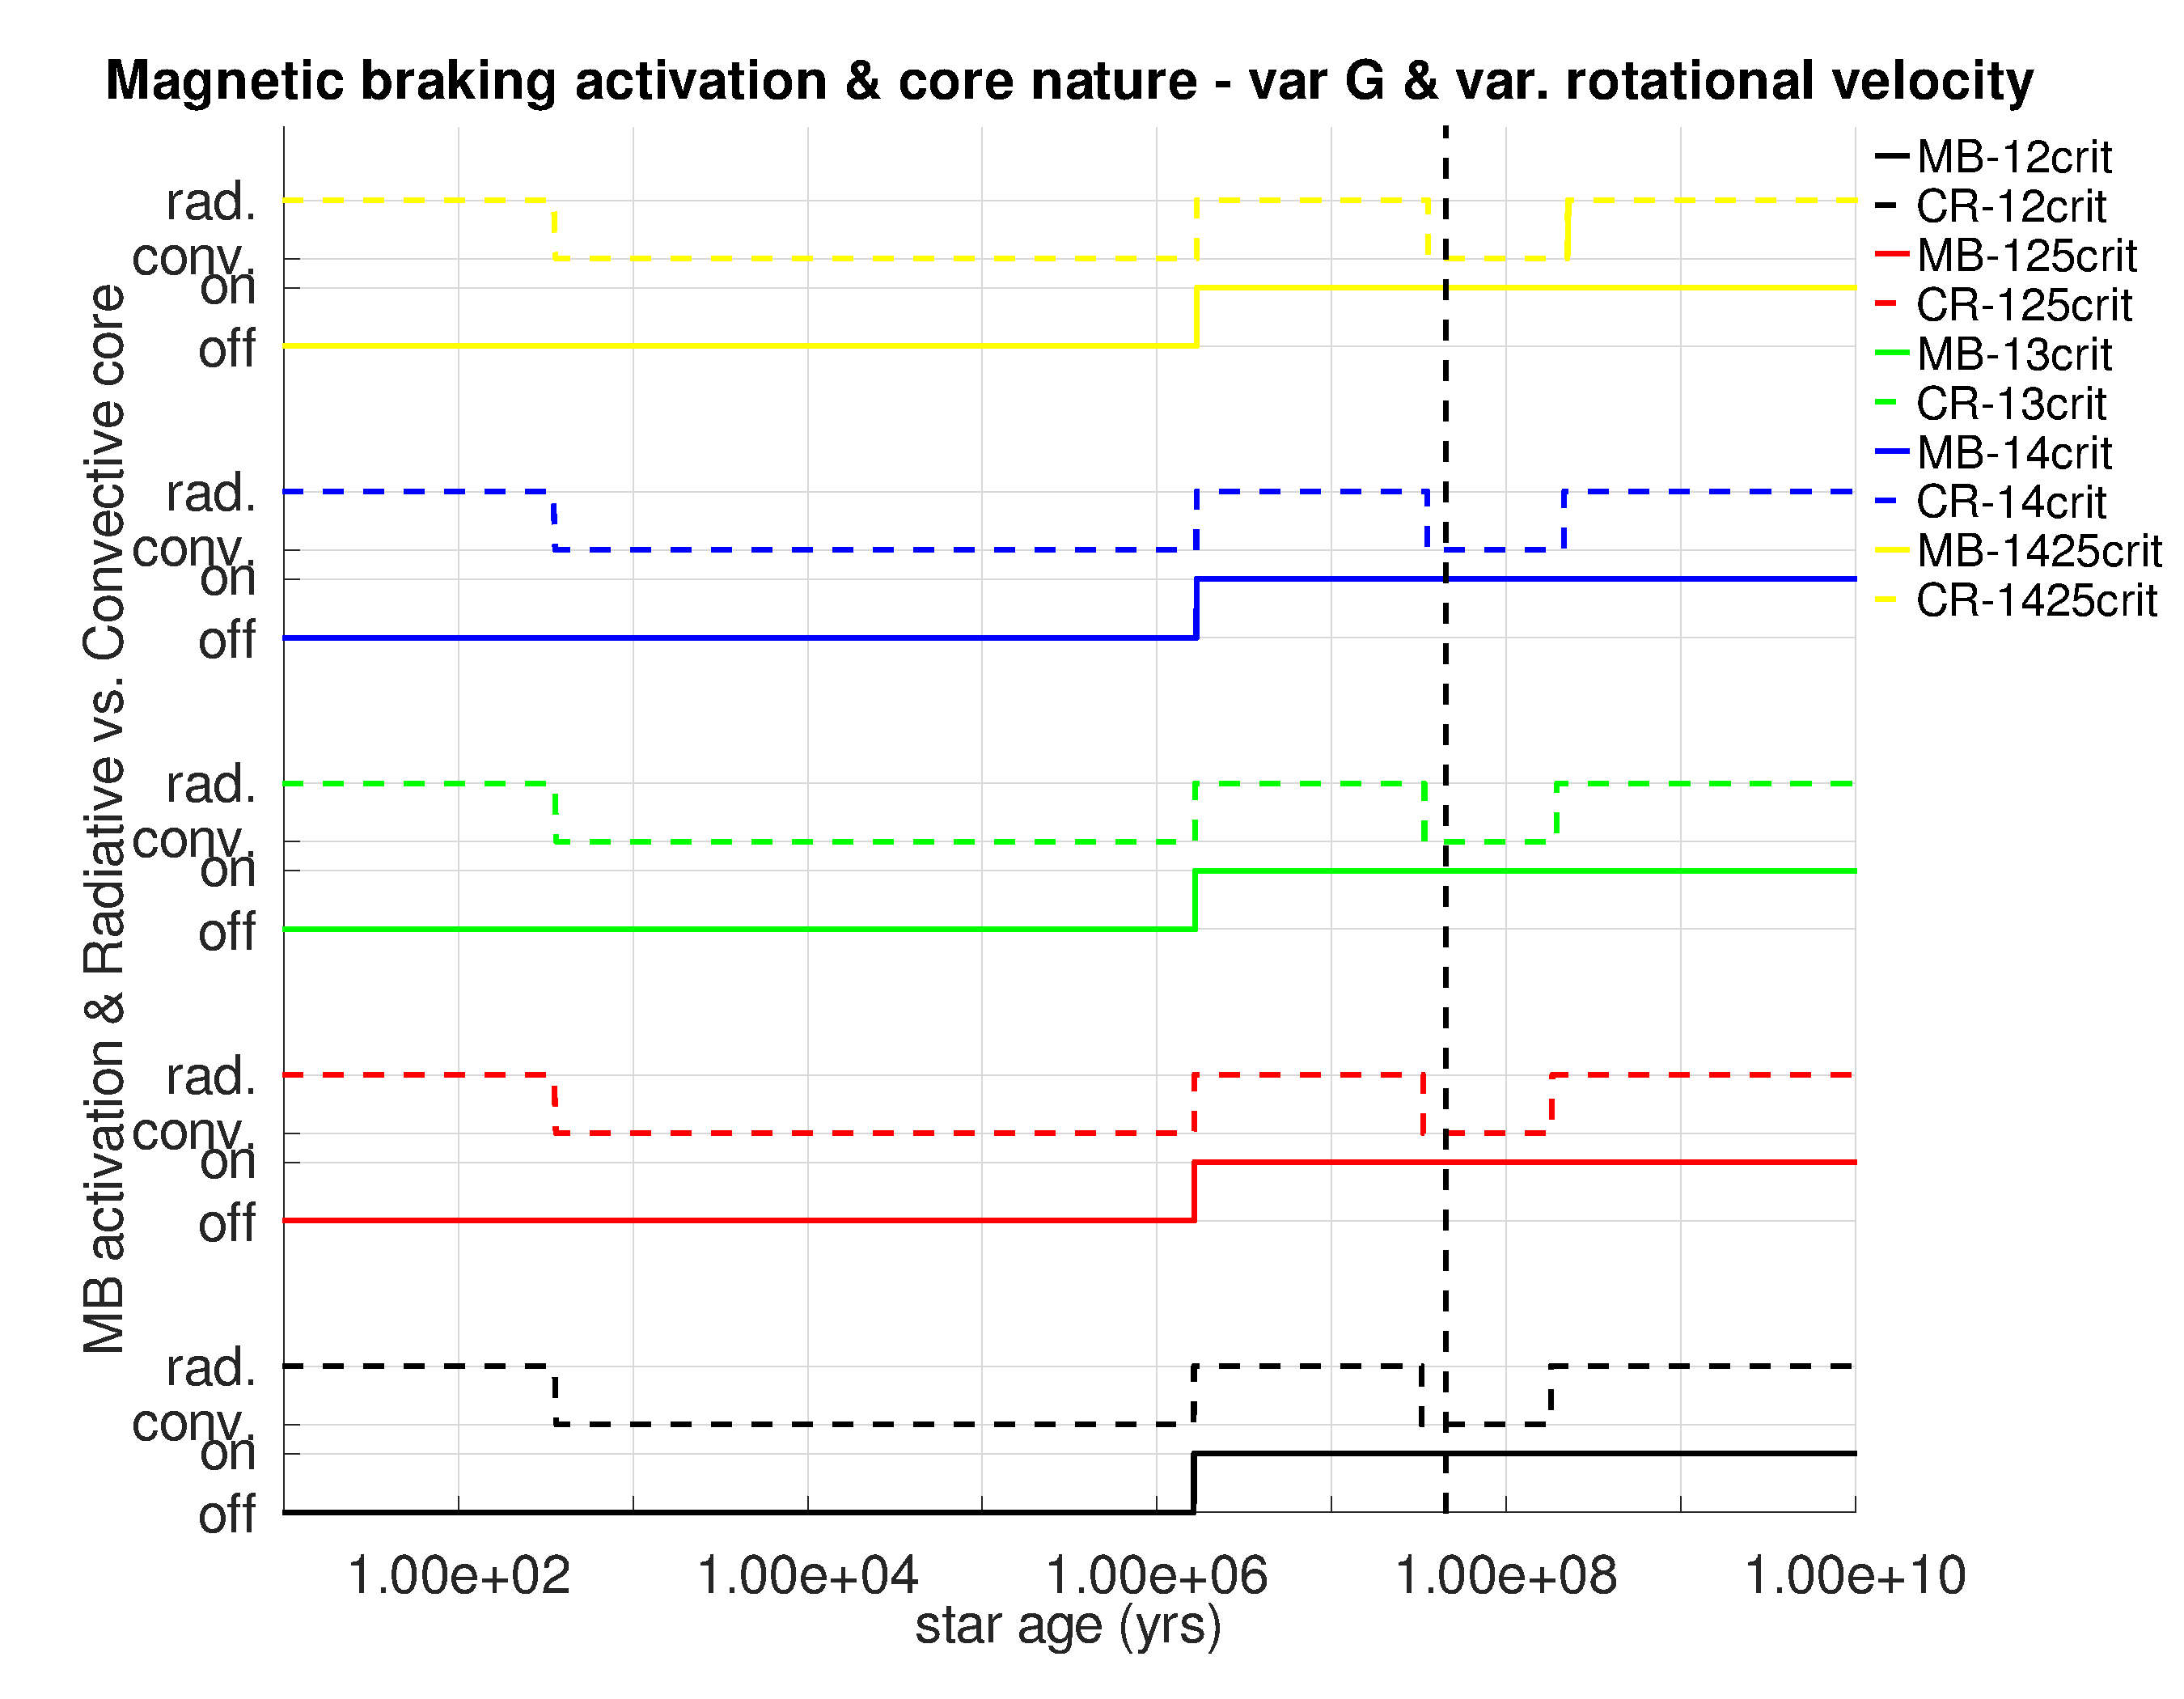
\includegraphics[clip,width=\columnwidth]{figures/paper2/mb_act_var_vel_g3.pdf}
    \caption{The activation of the magnetic braking routine as a function of the presence of a radiative core. The models include a magnetic field with variable intensity, PMS rotation with $\oomegac$ between 0.12 and 0.1425. The solid lines signal the magnetic braking routine activation (on) and deactivation (off). The horizontal dashed lines inform about the star's core nature: radiative (rad) or convective (conv). By implementation decision, once the routine is activated, it remains on even if the star's core nature change to convective. The dashed vertical line makes reference to the ZAMS.}
    \label{fig:mb_act_var_vel_g3}
\end{figure}

The effects of rotation and magnetic braking can also be seen in the H-R diagram and in the evolution of the $\amlt$. The inclusion of rotation implies the appearance of centrifugal forces that affect both the structure of the star, the chemical composition of the different strata that compose it, as well as its temperature and luminosity. The differential rotation between the boundaries of the radiative core and the convective layers leads to mixing effects in the so-called tachocline. The effects of this mixing and of its hydrostatic effects are governed by the MLT in which the $\amlt$ plays a major role in it. As aforementioned, MLT suffers from the arbitrariness of the value of $\amlt$, and it was necessary to establish its value based on physical constraints occurring in the interior of the star. Figure \ref{fig:alpha_mlt_var_vel_g3} shows how the $\amlt$ parameter evolves over time.\par 

\begin{figure}
	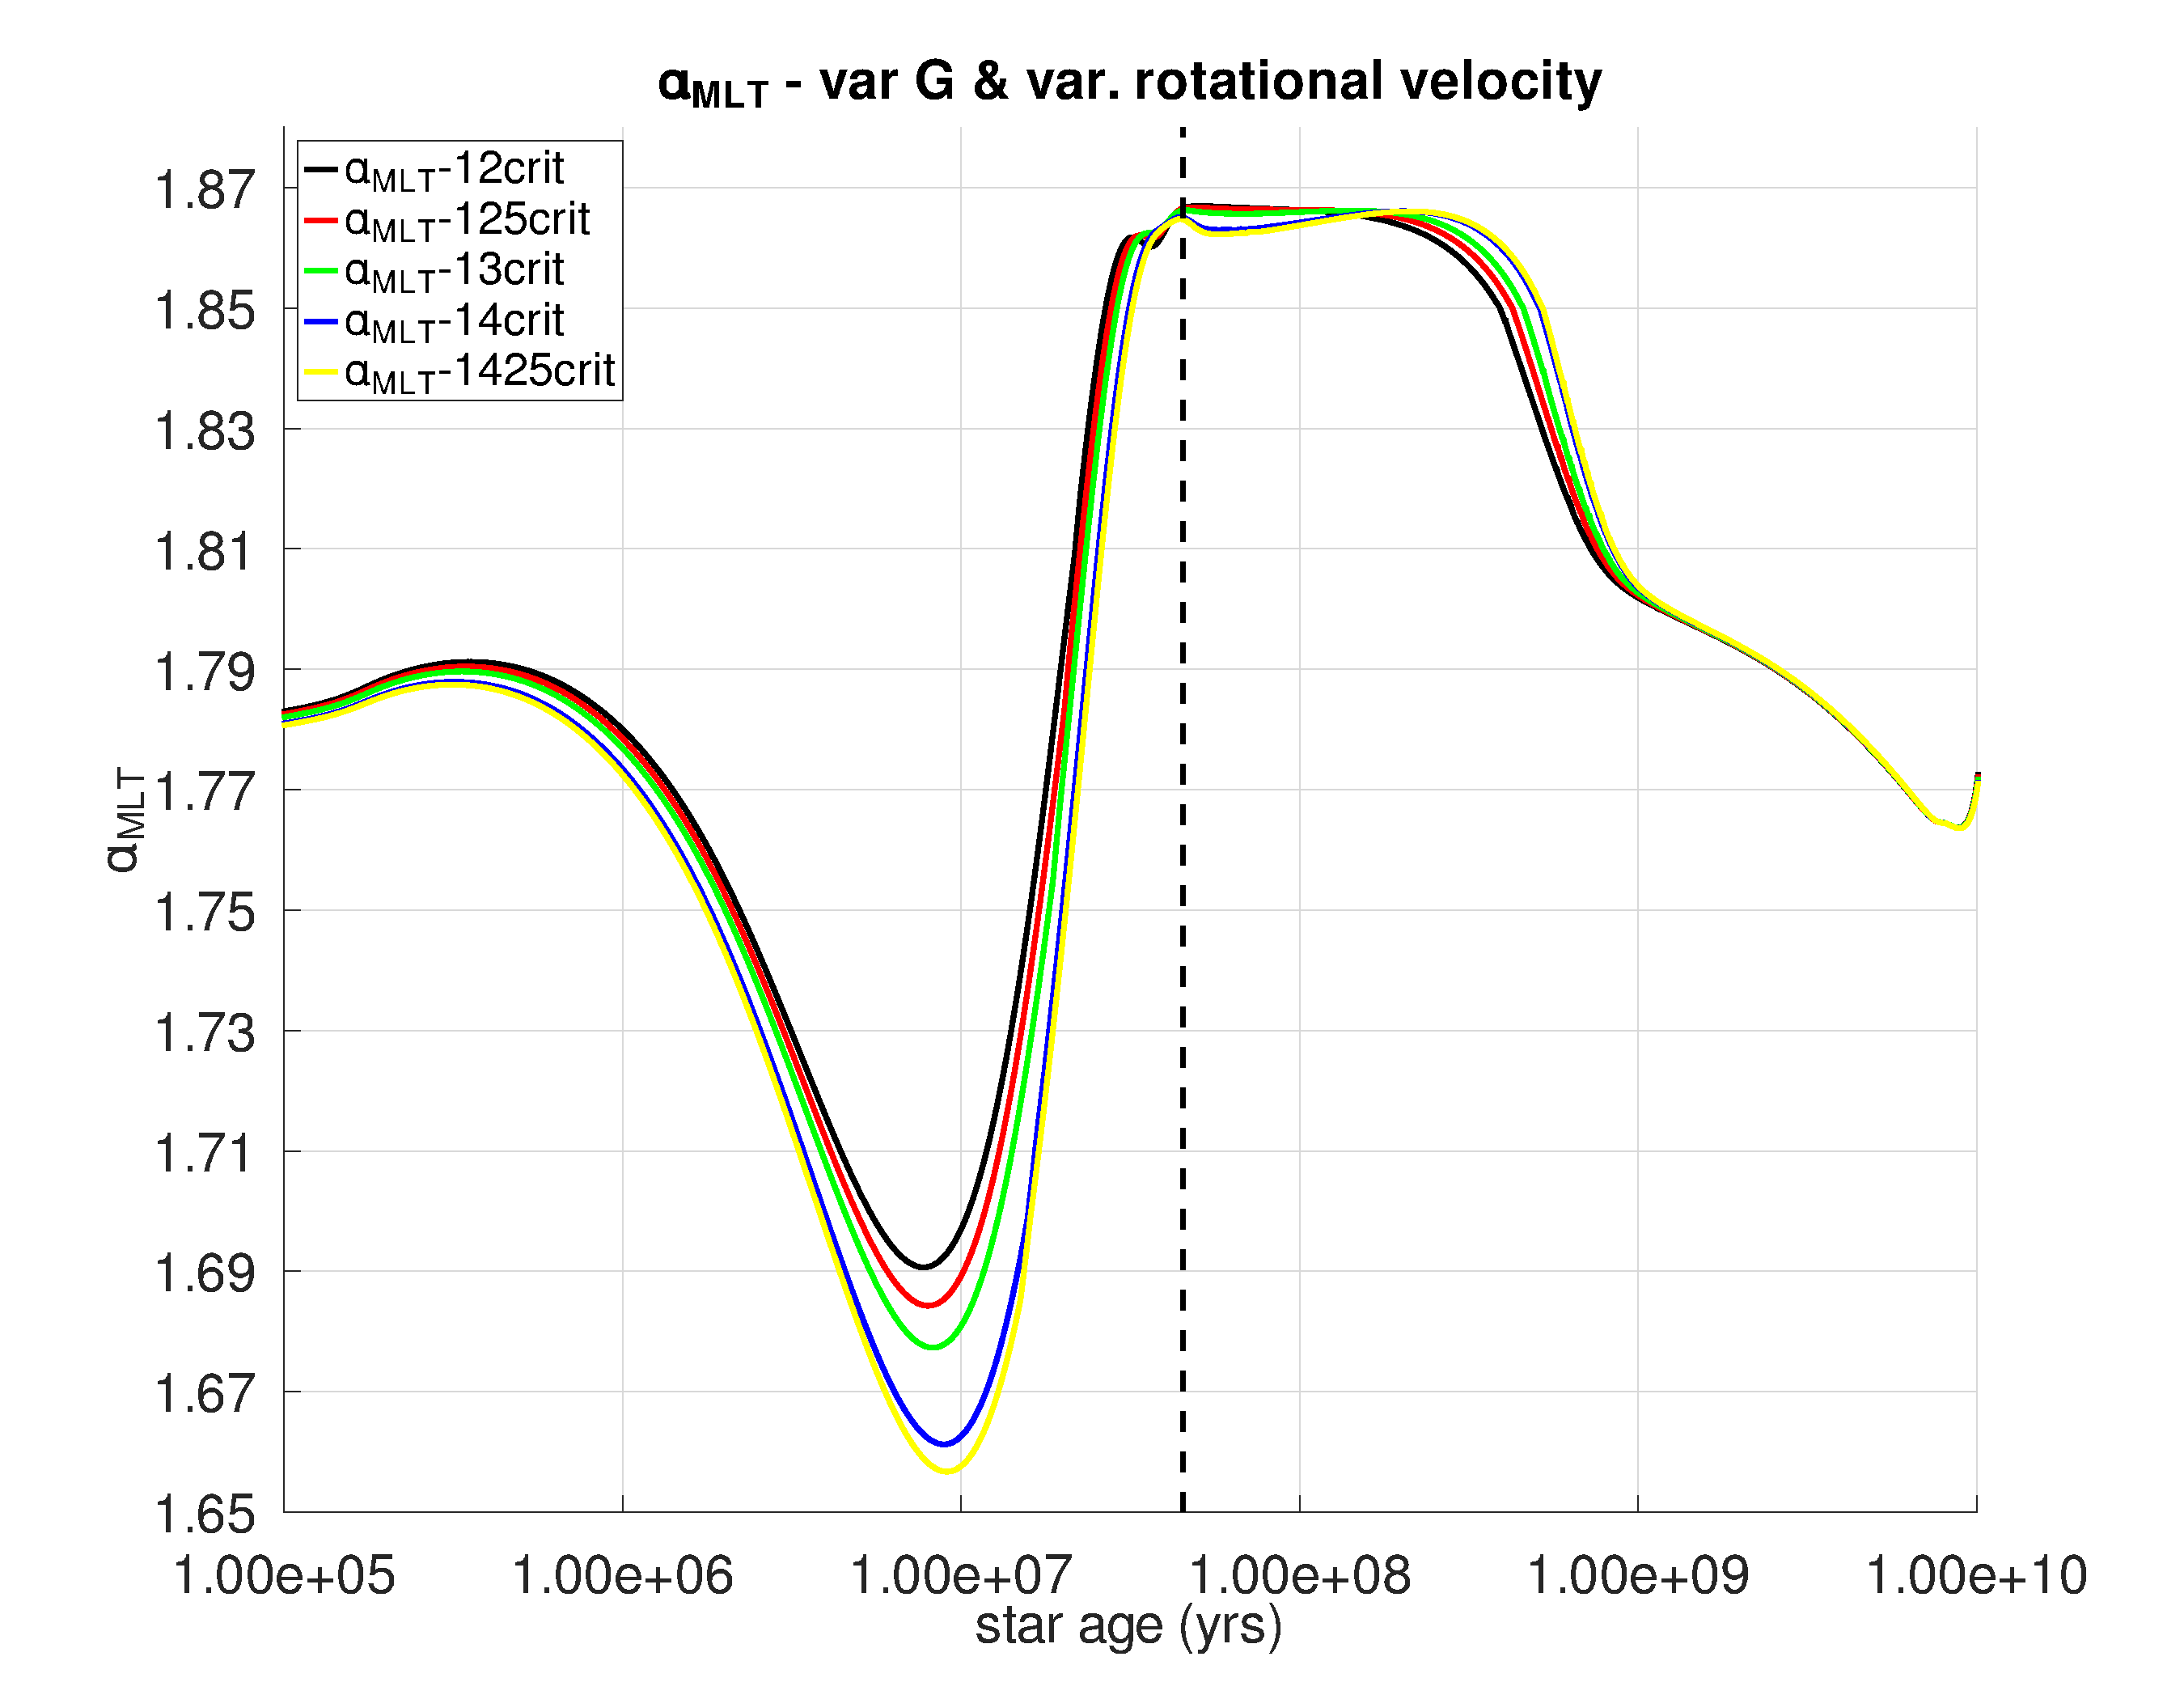
\includegraphics[clip,width=\columnwidth]{figures/paper2/alpha_mlt_var_vel_g3.pdf}
    \caption{The evolution of $\amlt$, as a function of time and $\oomegac$ for several 1 $\msun$ models and their. The models include PMS rotation with $\oomegac$ between 0.12 and 0.1425. The dashed vertical line makes reference to the ZAMS.}
    \label{fig:alpha_mlt_var_vel_g3}
\end{figure}

Additionally, these same centrifugal forces, accentuated in stars with a higher angular velocity, reinforce the gravity darkening \citep[see e.g. ][]{Gossage2021,Paxton2019,Eggenberger2012} as well. The centrifugal force causes the star to shift its mass outwards with respect to the rotation axis, the effect being more pronounced in the equatorial regions than at the poles. The consequence is that the pressure ($\gsurf$) to which the gas is subjected is lower in the former than in the latter. This effect causes those stars that rotate fast enough to appear less dense ($\rho$), less luminous ($L$) and therefore with a lower effective temperature ($\teff$) as they approach the ZAMS (see Figure \ref{fig:hr_var_vel_var_g_z13}). If we compare the non-rotating model (black solid line in Figure \ref{fig:hr_var_vel_0g}) with the rotating ones we can recognize that at the end of the PMS, the latter reach the ZAMS with a lower $\teff$ than the former. This also has an impact on the evolution of $\amlt$ because, as discussed above, in our model its value depends proportionally on $\teff$ and $\gsurf$. Both parameters are comparatively smaller for stars that rotate faster than for those that rotate more slowly. As a consequence $\amlt$ yields a lower value in its time evolution in those phases in which the star rotates faster, being this effect more accentuated in the ZAMS approach.\par

\begin{figure}
	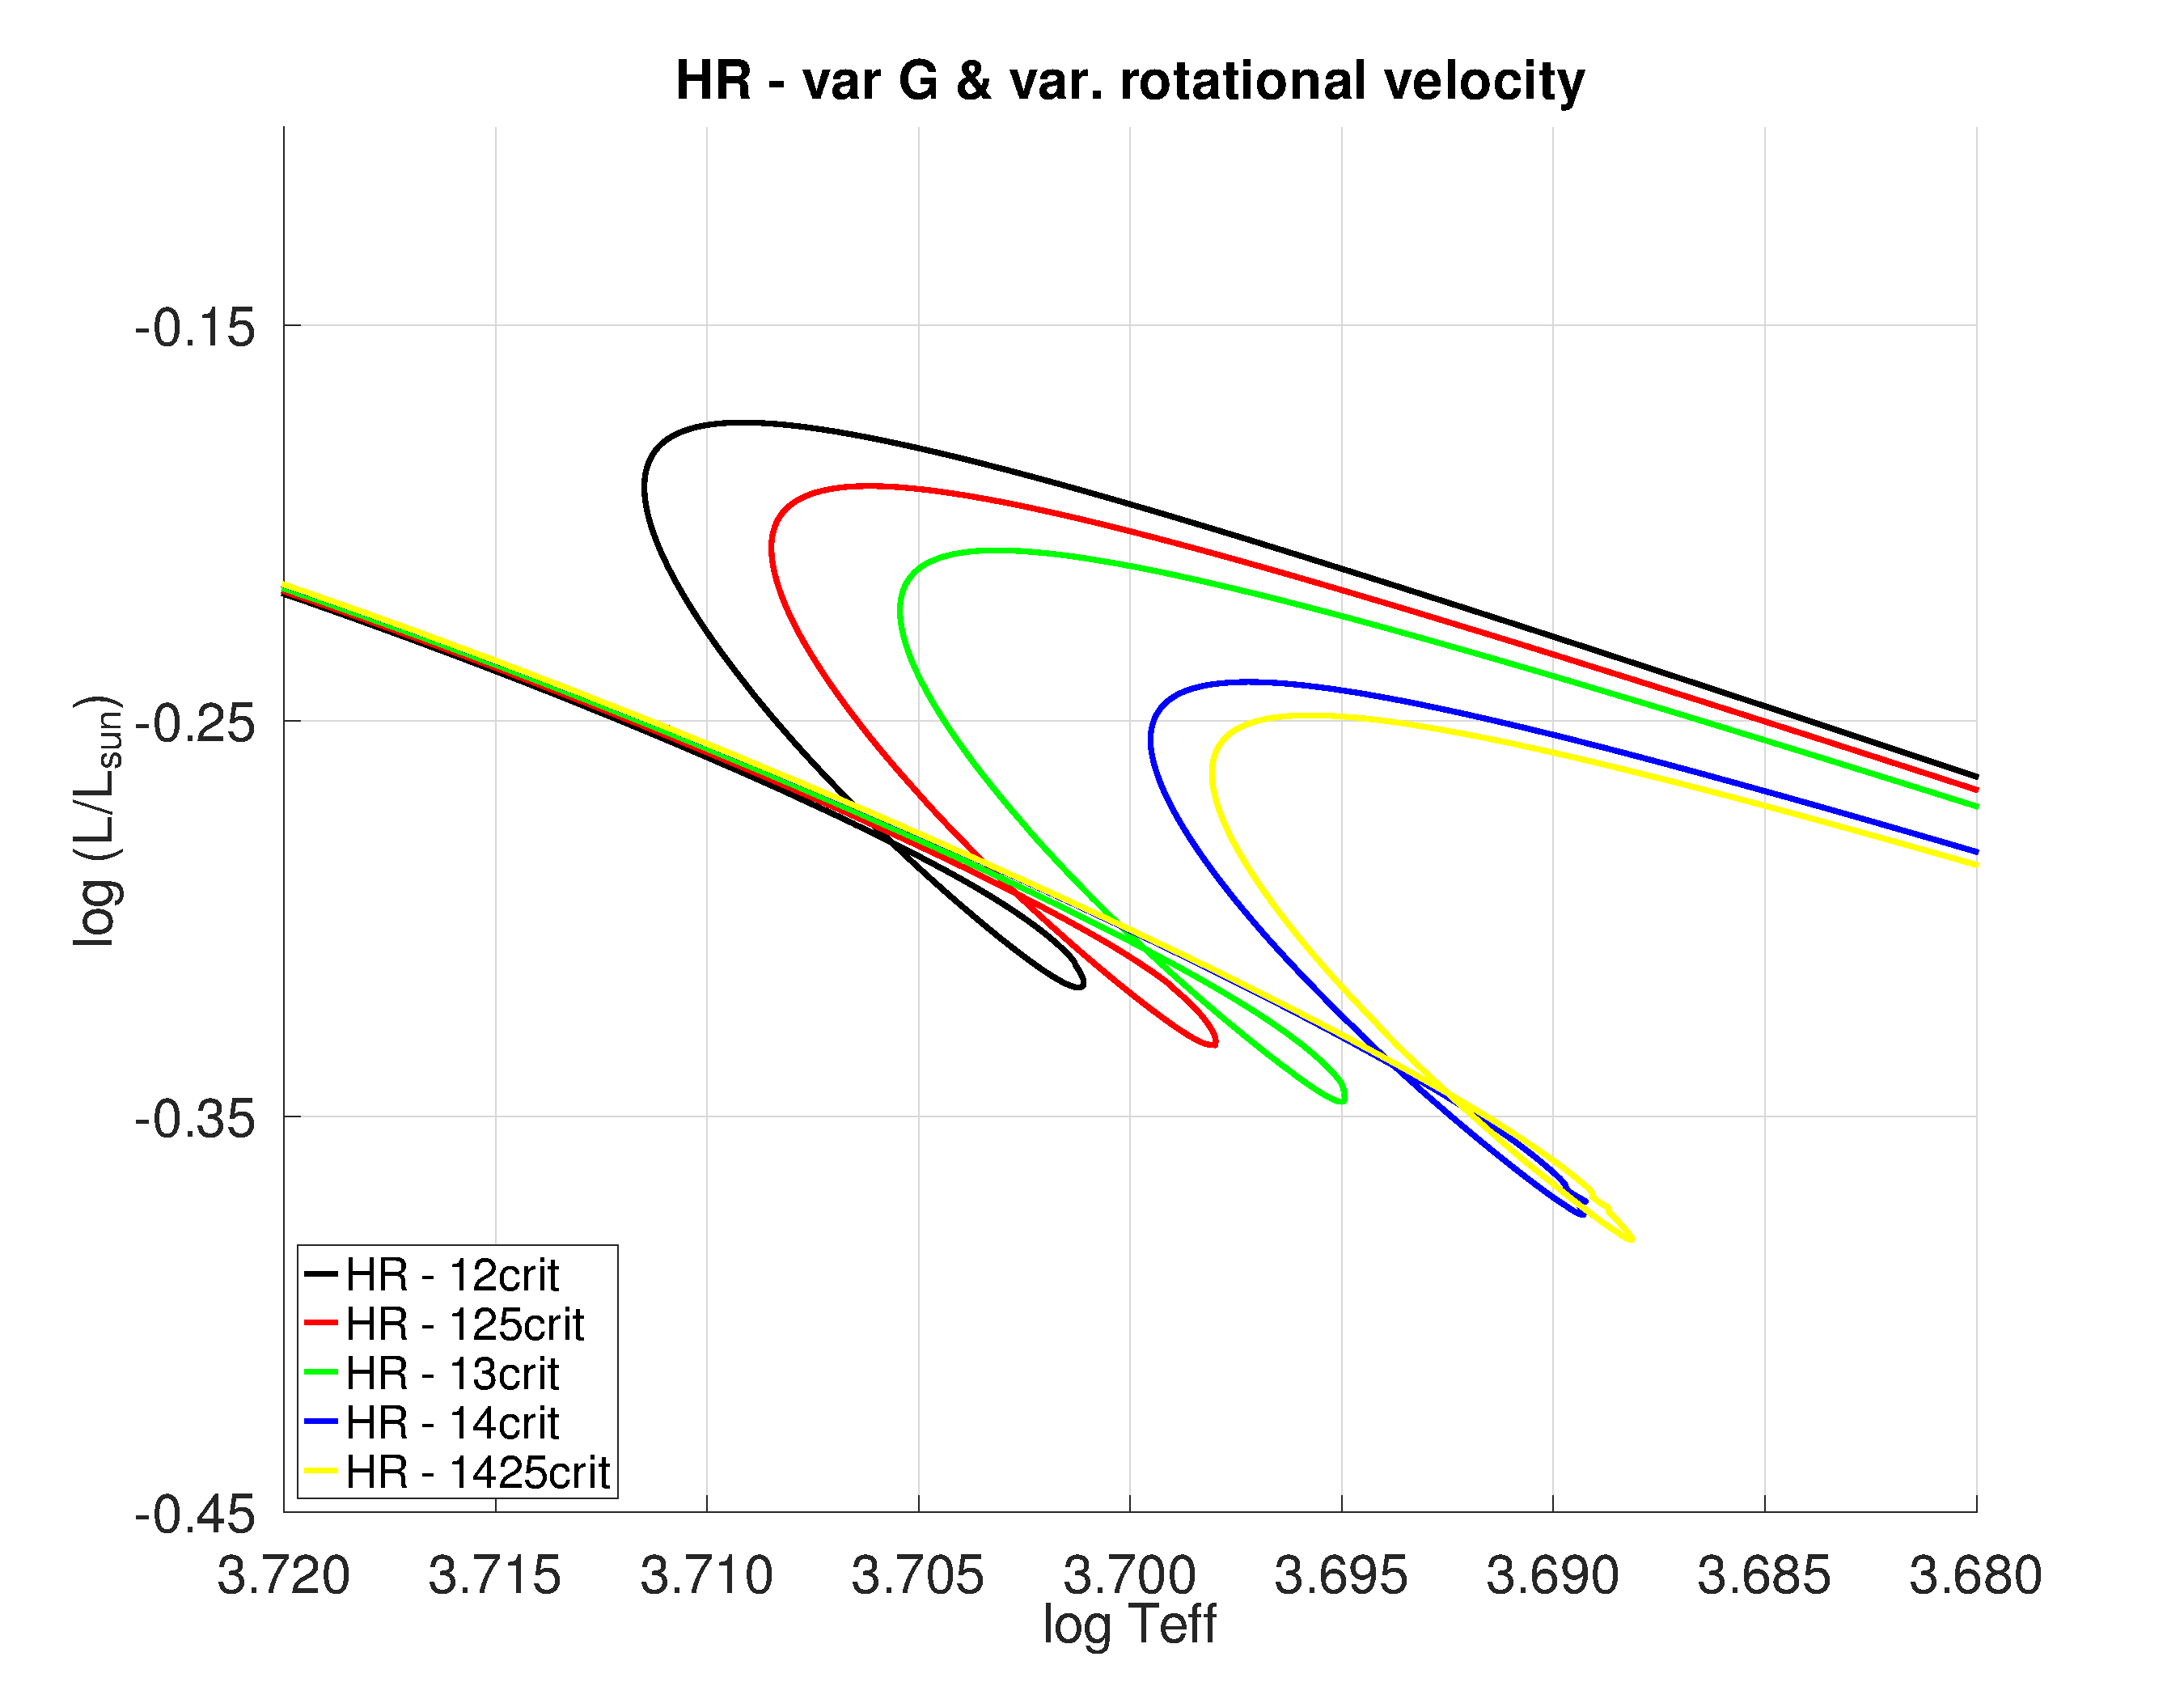
\includegraphics[clip,width=\columnwidth]{figures/paper2/hr_var_vel_var_g_z13.pdf}
    \caption{Similar to Figure \ref{fig:hr_var_vel_0g} but now showing in detail the combined effects of the gravity darkening and magnetic braking on the evolutionary tracks for several 1 $\msun$ models. The models include a magnetic field with variable intensity, PMS rotation with $\oomegac$ between 0.12 and 0.1425. The presence of a magnetic field produces hotter stars due to the influence of the magnetic braking on the rotational velocity of the star. $\lsun$ = 3.761.}
    \label{fig:hr_var_vel_var_g_z13}
\end{figure}

\begin{figure}
	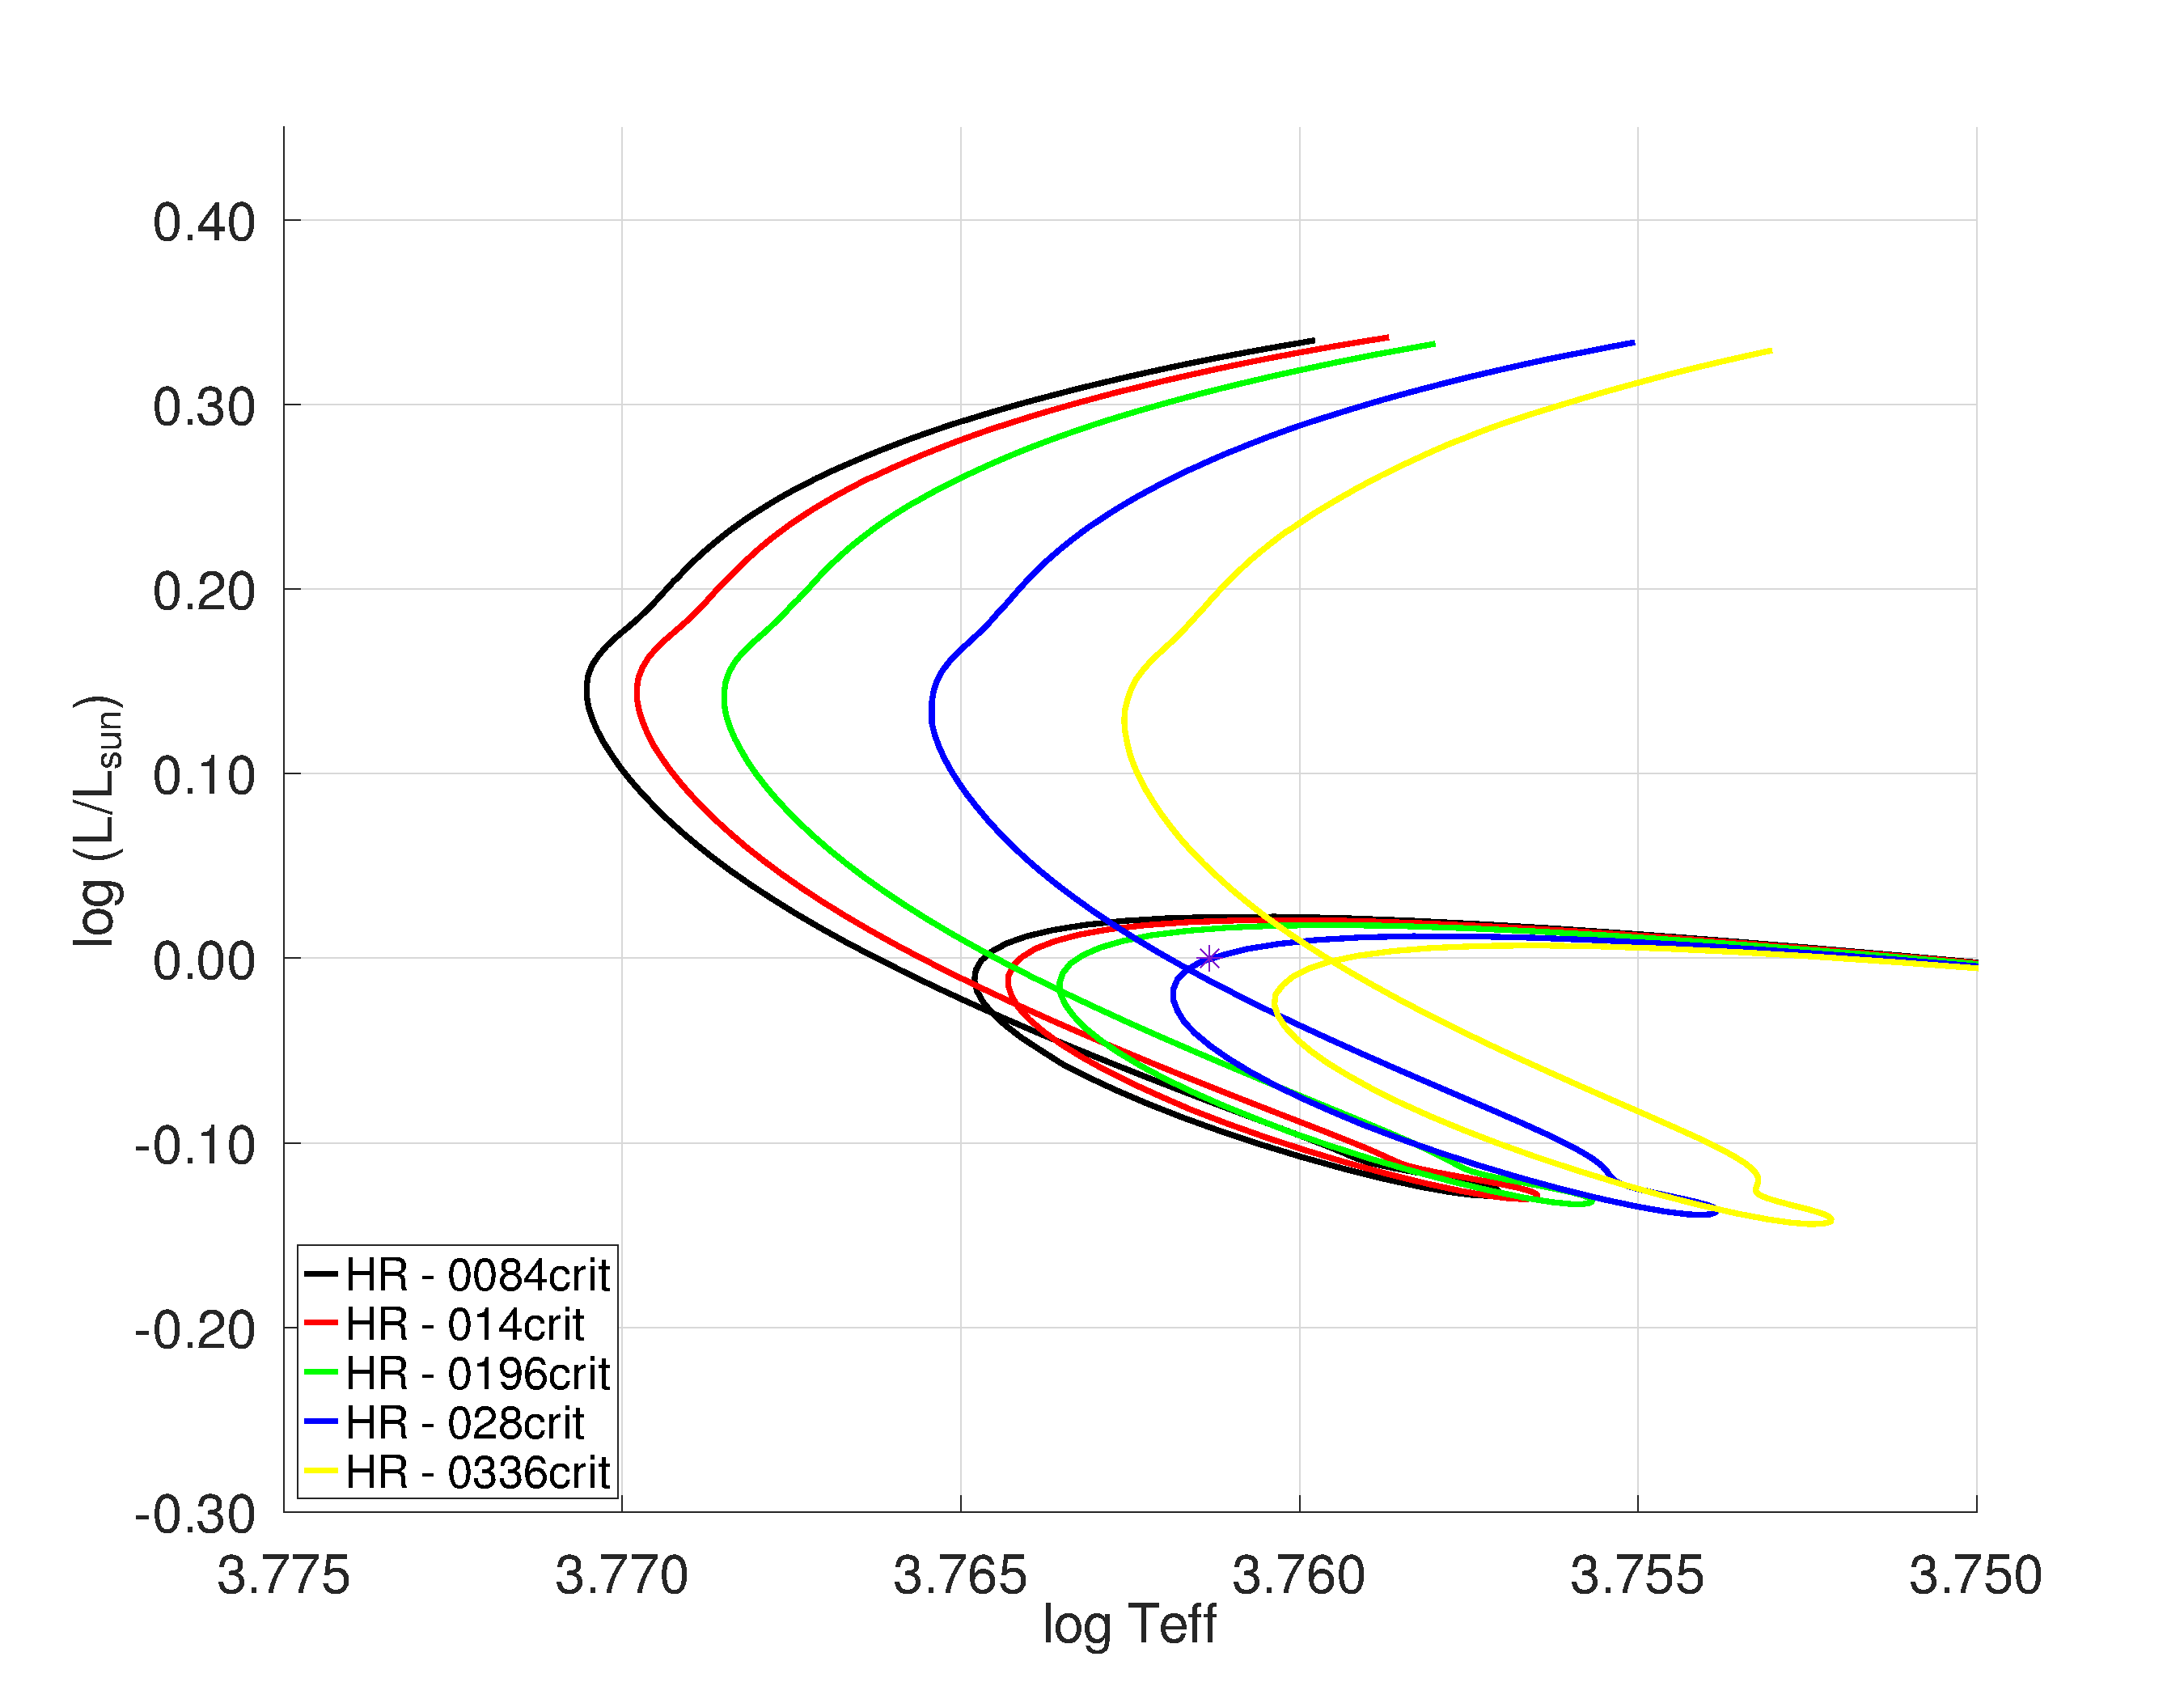
\includegraphics[trim = 10mm 10mm 15mm 10mm, clip,width=\columnwidth]{figures/paper2/hr_var_vel_0_0g_z10.pdf}
    \caption{An example solar 1$\msun$ grid of stellar evolutionary track from PMS till TAMS covering a wide range of angular velocities. The rotation is activated in the models in the PMS and those models reach before the ZAMS and at a lower $\teff$ than the non-rotating one (solid black line). The luminosity is expressed in terms of $\lsun$. (Figure taken from \citet{Navarro2020}.)}
    \label{fig:hr_var_vel_0g}
\end{figure}

Figures \ref{fig:teff_logg_var_vel_g3} and \ref{fig:teff_logg_var_vel_g_z13} show how $\teff$ and $\gsurf$ behave over the evolution of the models. For those with a higher rotation speed we observe that both their temperature and surface gravity are lower than in the slower rotating models, in line with the gravity darkening. It is worth noting that in the ZAMS approach phase we observe for the faster rotating model (yellow) that its surface gravity is higher than that of the rest of the slower models. This can be explained by looking at Figure \ref{fig:mdot_var_vel_g3}, which shows the mass loss of the star. Around the interval $2.5x10^{7}$ and $3.5x10^{7}$ years the mass loss of the fastest model is smaller than that of the rest. Since the surface gravity is directly proportional to the amount of mass of the star, if the mass of the star decreases, the surface gravity decreases as well. During this period the faster model does so at a lower rate and so we have a higher surface gravity. This "anomaly" disappears as soon as the mass loss becomes more pronounced and becomes noticeably larger between $3.5x10^{7}$ and $4.5x10^{7}$ years, shortly before reaching ZAMS. In this phase the surface gravity of the fastest rotator is lower than that of the other models. We have a similar situation past ZAMS, from around $4.5x10^{7}$ till $11.0x10^{7}$ years. In this case the explanation for the higher surface gravity of the model that rotates faster than the others is due to the size of the star, how its radius behaves. Figures \ref{fig:lograd_var_vel_g3} and \ref{fig:lograd_var_vel_g_z13} show the time evolution of the radius for the different models. In them we can see how for the fastest rotator, in the above-mentioned time interval, its size is smaller. As it decreases more than the others, and although it also continues to lose more mass, its $\gsurf$ is greater. Let us remember that the radius has an inversely quadratic influence on the value of the $\gsurf$.\par


\begin{figure}
	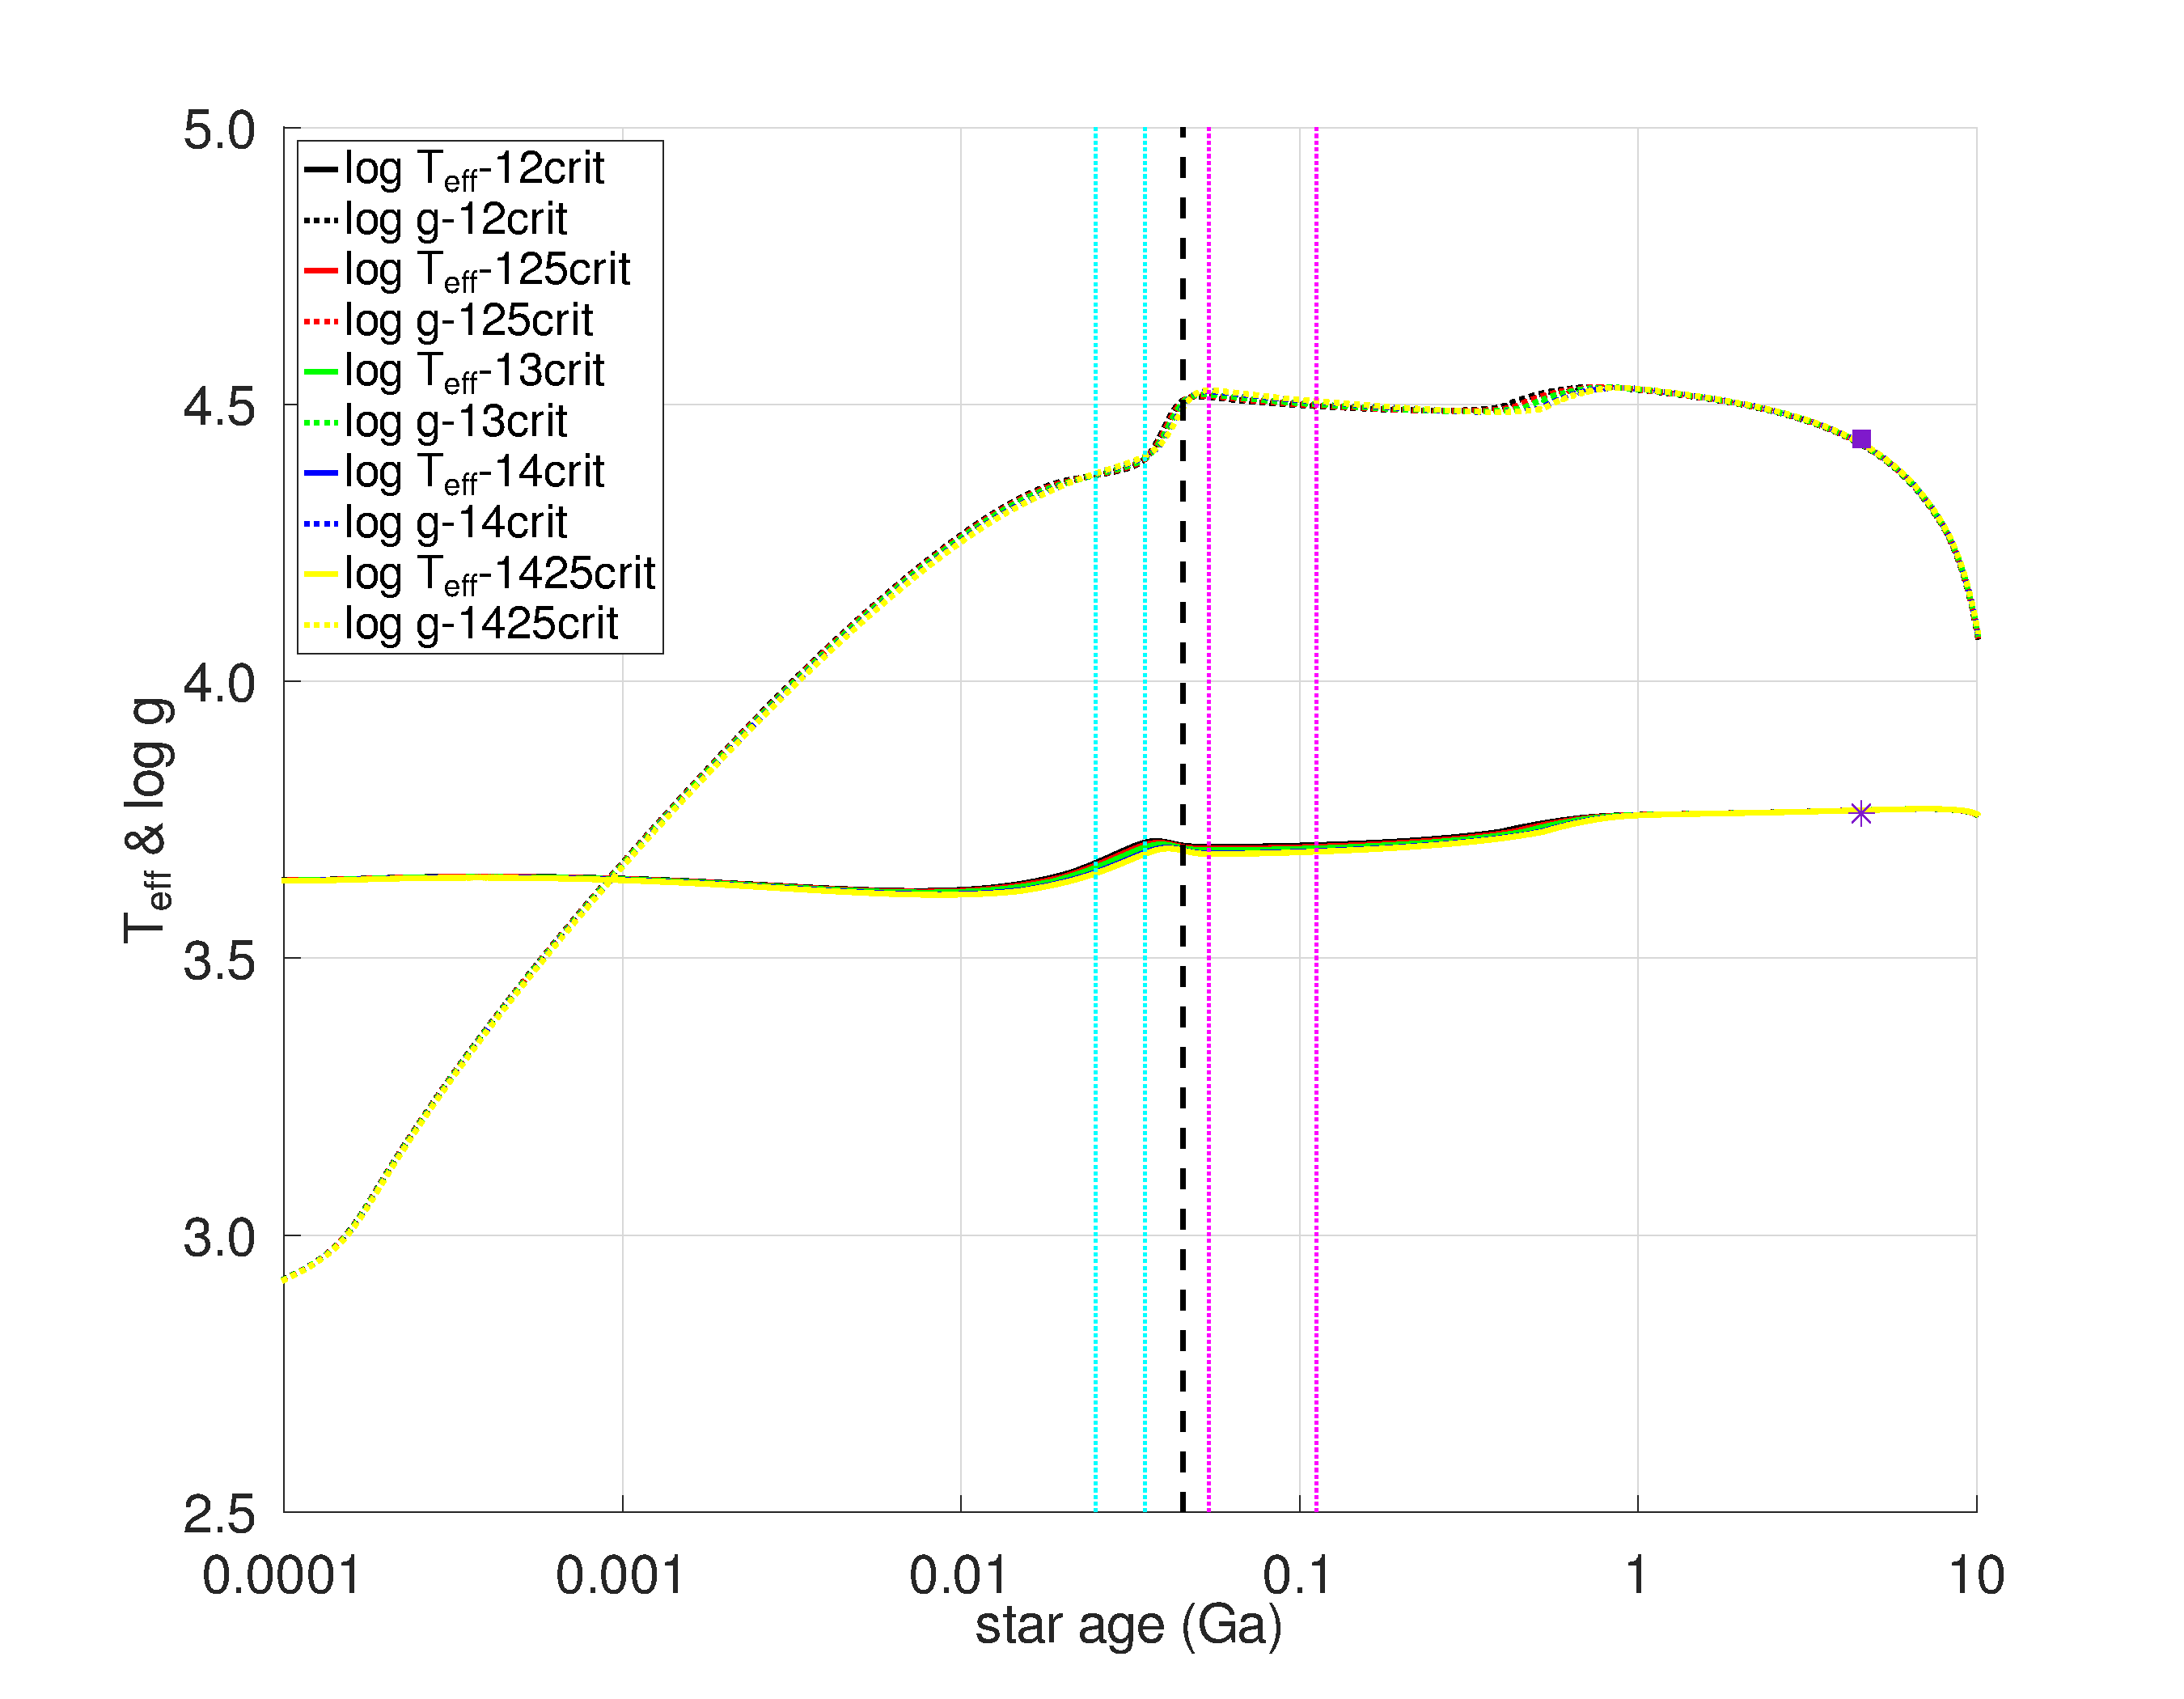
\includegraphics[clip,width=\columnwidth]{figures/paper2/teff_logg_var_vel_g3.pdf}
    \caption{The evolution of $\teff$ and $\gsurf$, as a function of time and $\oomegac$ for several 1 $\msun$ models and their. The models include PMS rotation with $\oomegac$ between 0.12 and 0.1425. The purple star is the $\teff$, and the purple square is the $\gsurf$ for the present-day Sun \citep{Gill2012}. The dashed vertical line makes reference to the ZAMS.}
    \label{fig:teff_logg_var_vel_g3}
\end{figure}

\begin{figure}
	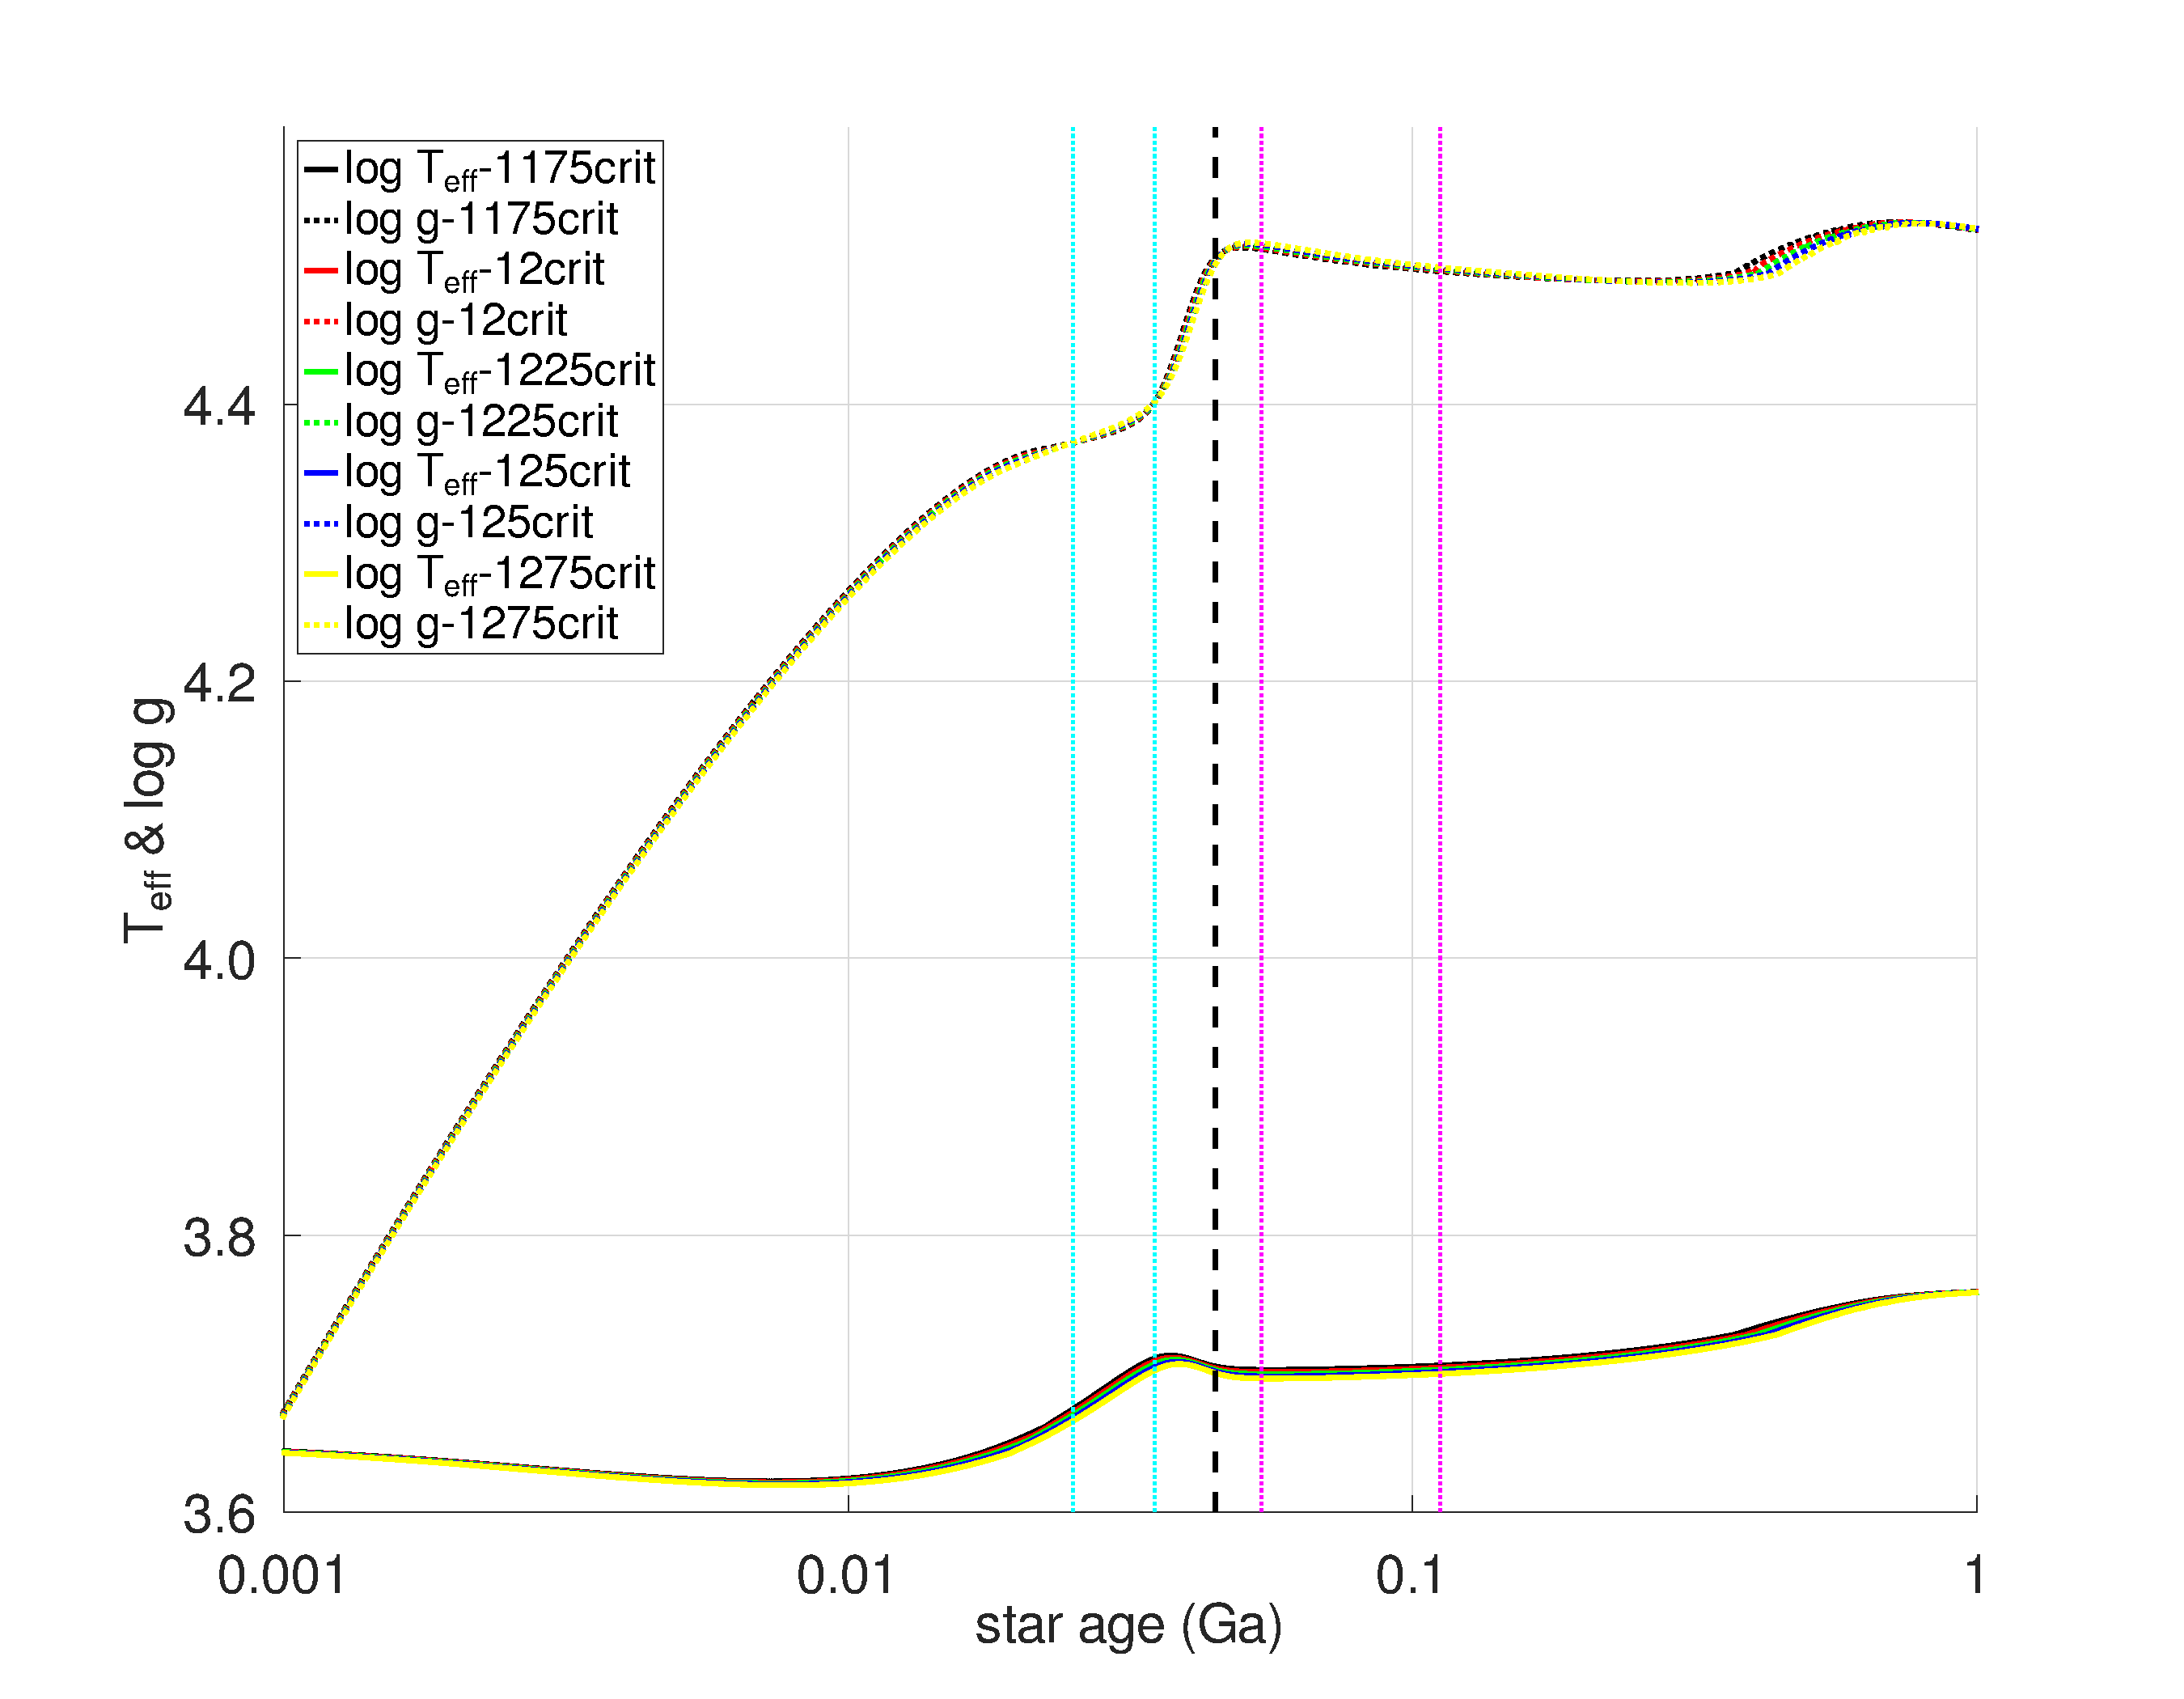
\includegraphics[clip,width=\columnwidth]{figures/paper2/teff_logg_var_vel_g_z13.pdf}
    \caption{Similar to \ref{fig:teff_logg_var_vel_g3} but zooming in on the ZAMS. The models with a higher initial rotational velocity reach already the ZAMS with a lower $\teff$ and higher $\gsurf$.}
    \label{fig:teff_logg_var_vel_g_z13}
\end{figure}


\begin{figure}
	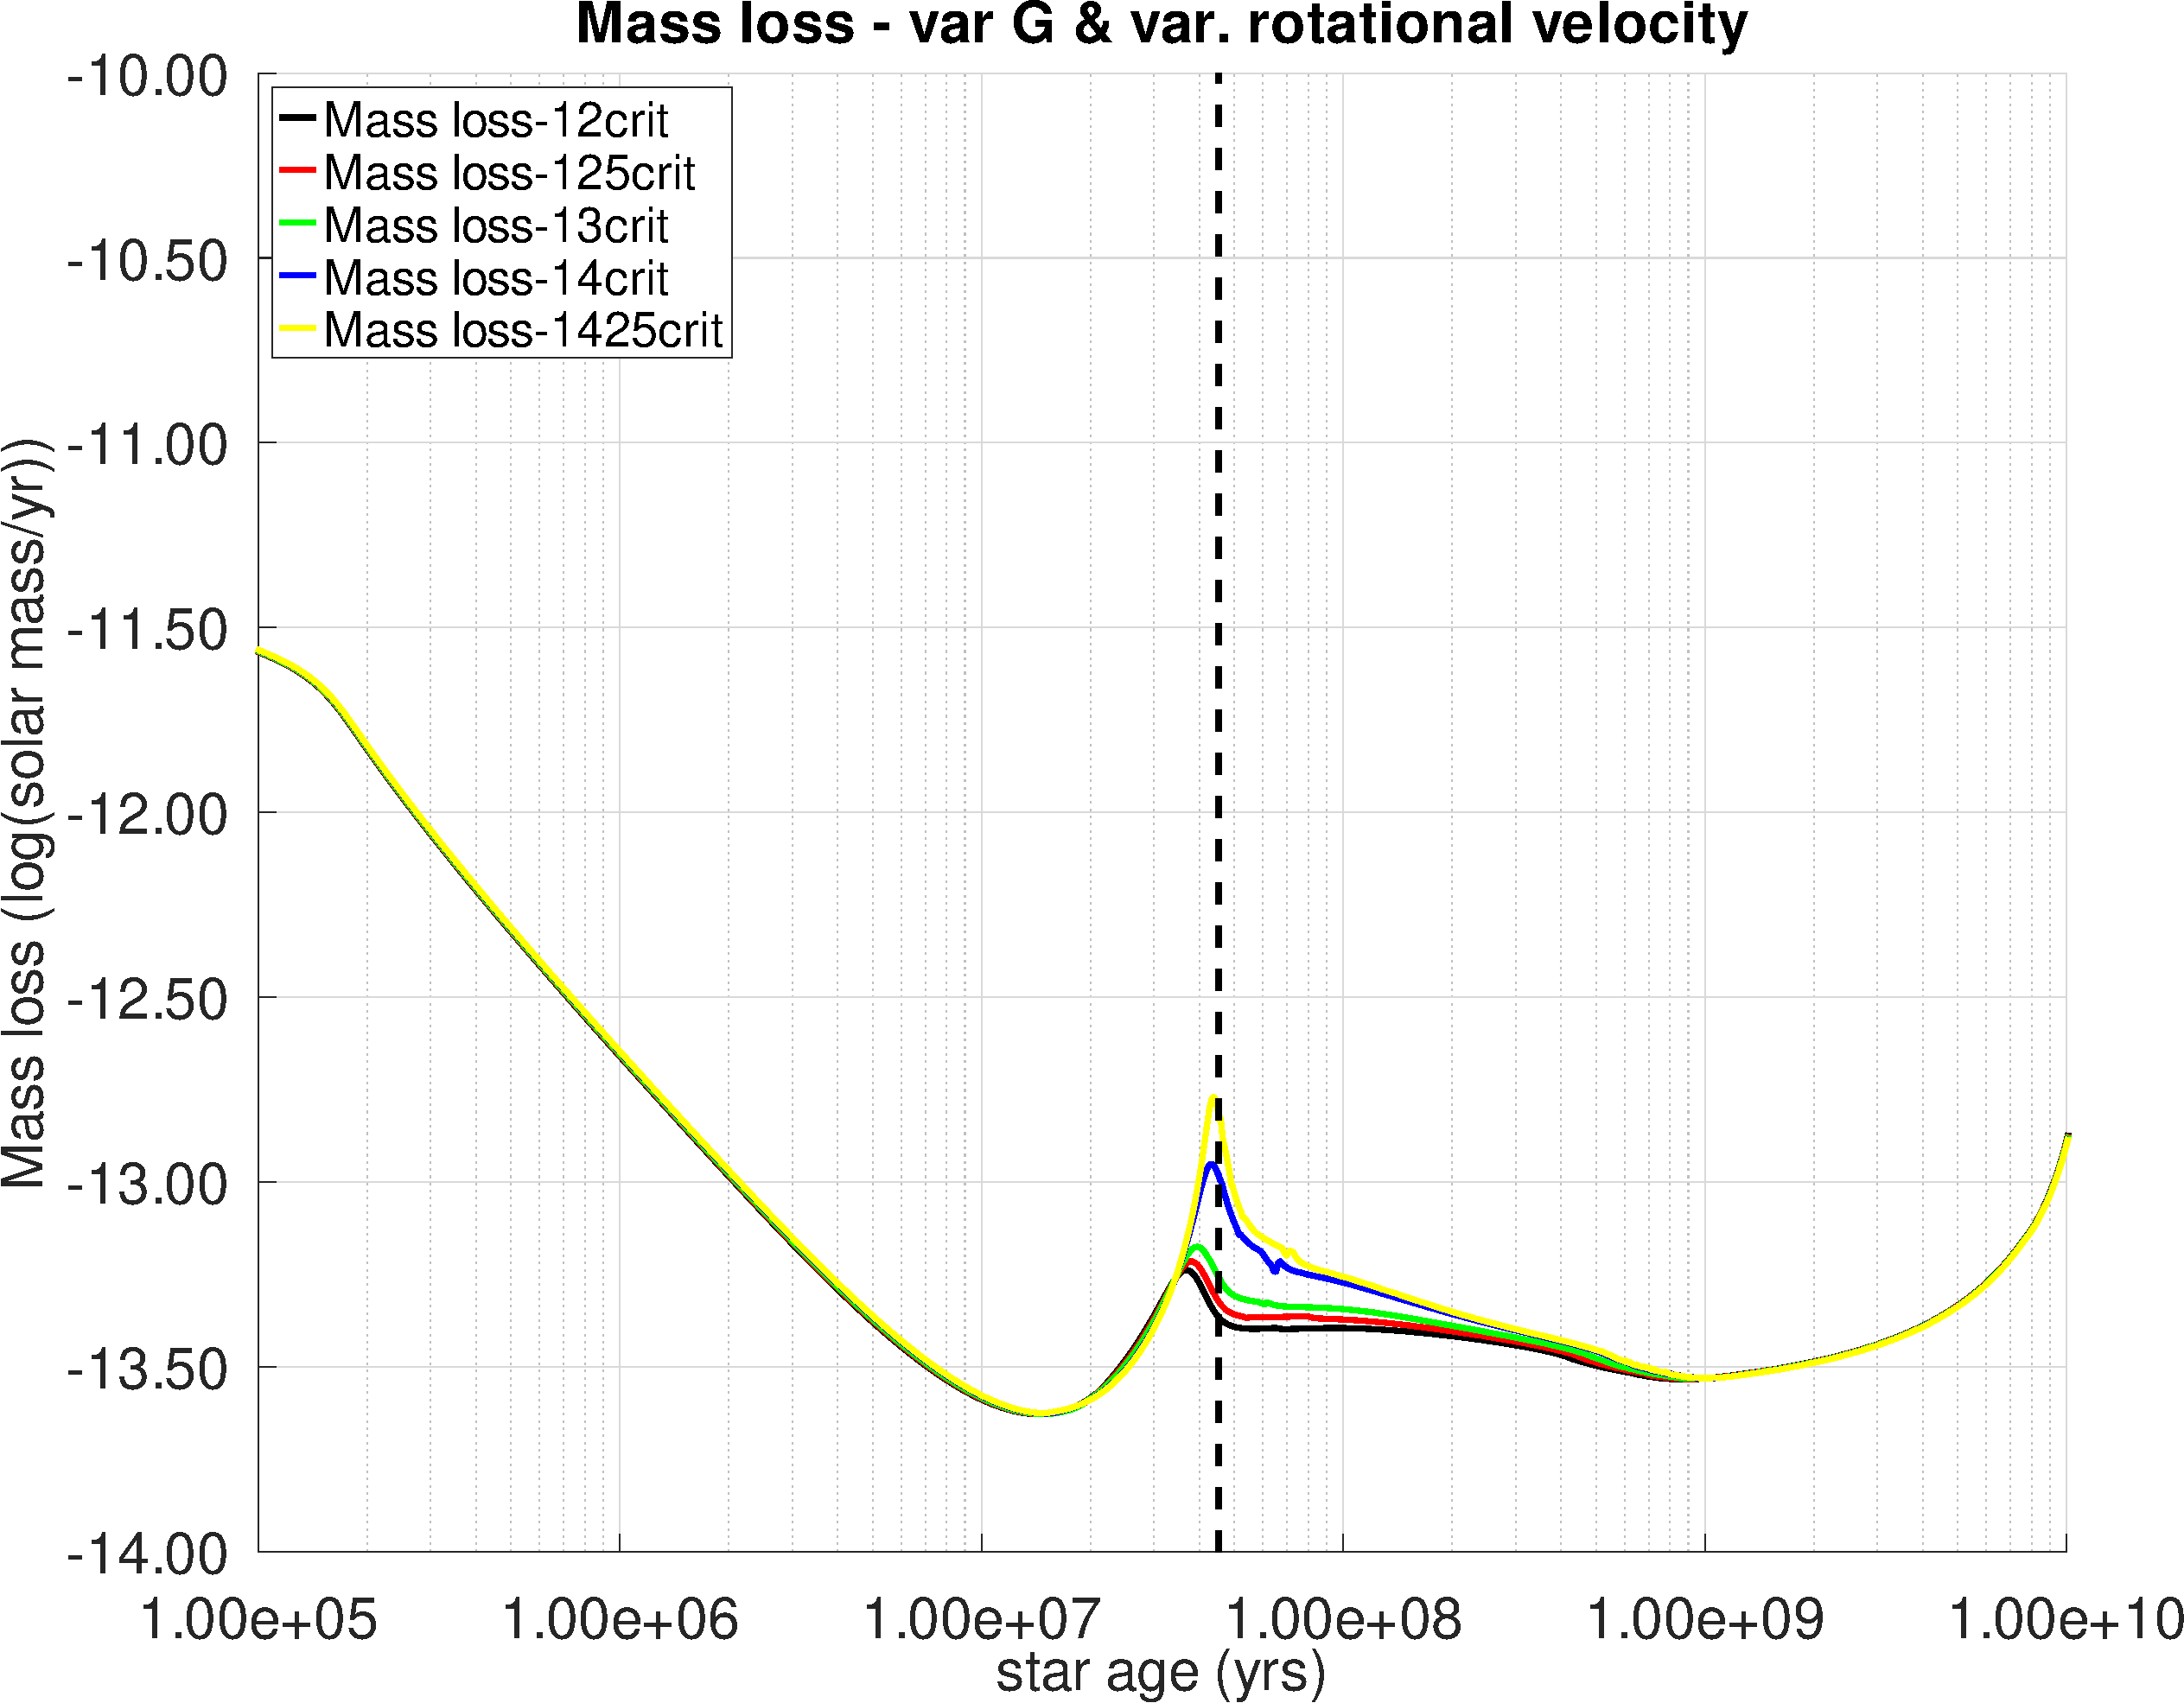
\includegraphics[clip,width=\columnwidth]{figures/paper2/mdot_var_vel_g3.pdf}
    \caption{The evolution of mass loss $\Dot{M}$ as a function of time for several 1 $\msun$ models. The models include variable magnetic field intensity and PMS rotation with $\oomegac$ between 0.12 and 0.1425. The dashed vertical line makes reference to the ZAMS.}
    \label{fig:mdot_var_vel_g3}
\end{figure}



\begin{figure}
	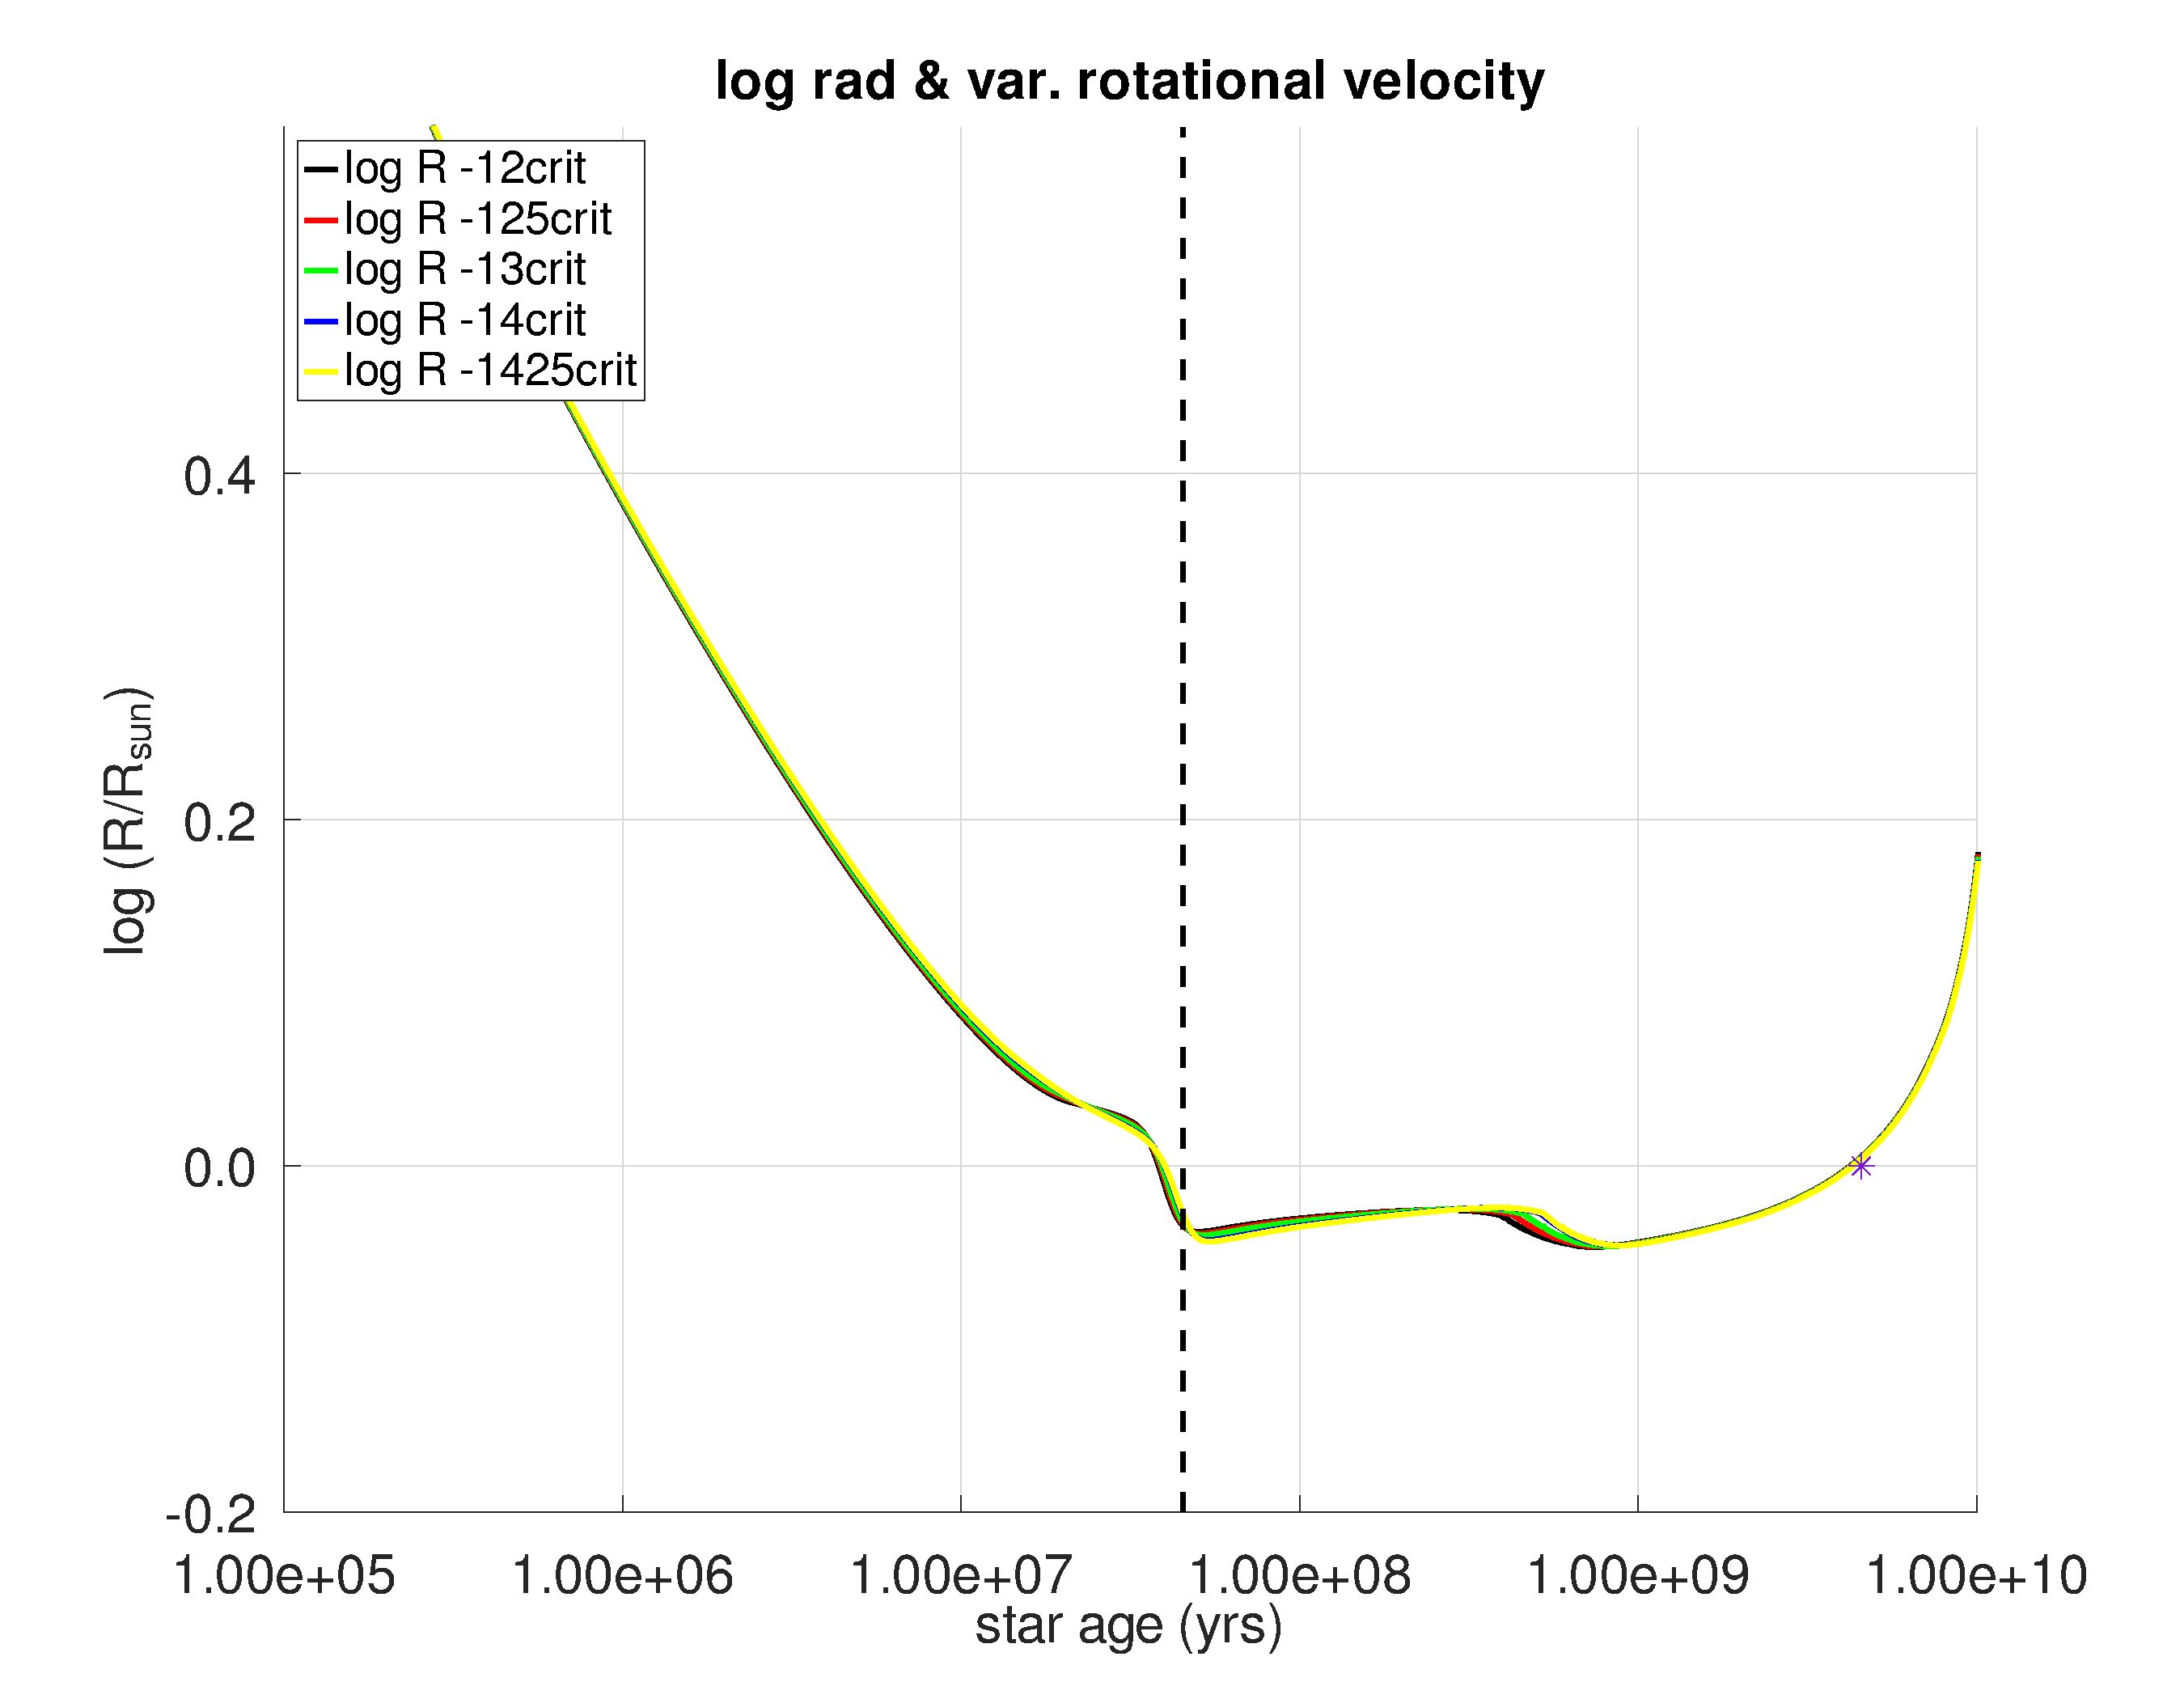
\includegraphics[clip,width=\columnwidth]{figures/paper2/lograd_var_vel_g3.pdf}
    \caption{The evolution of the stellar radius, as a function of time and $\oomegac$ for several 1 $\msun$ models and their. The models include PMS rotation with $\oomegac$ between 0.12 and 0.1425. The purple star is the radius for the present-day Sun \citep{Gill2012}. The dashed vertical line makes reference to the ZAMS.}
    \label{fig:lograd_var_vel_g3}
\end{figure}

\begin{figure}
	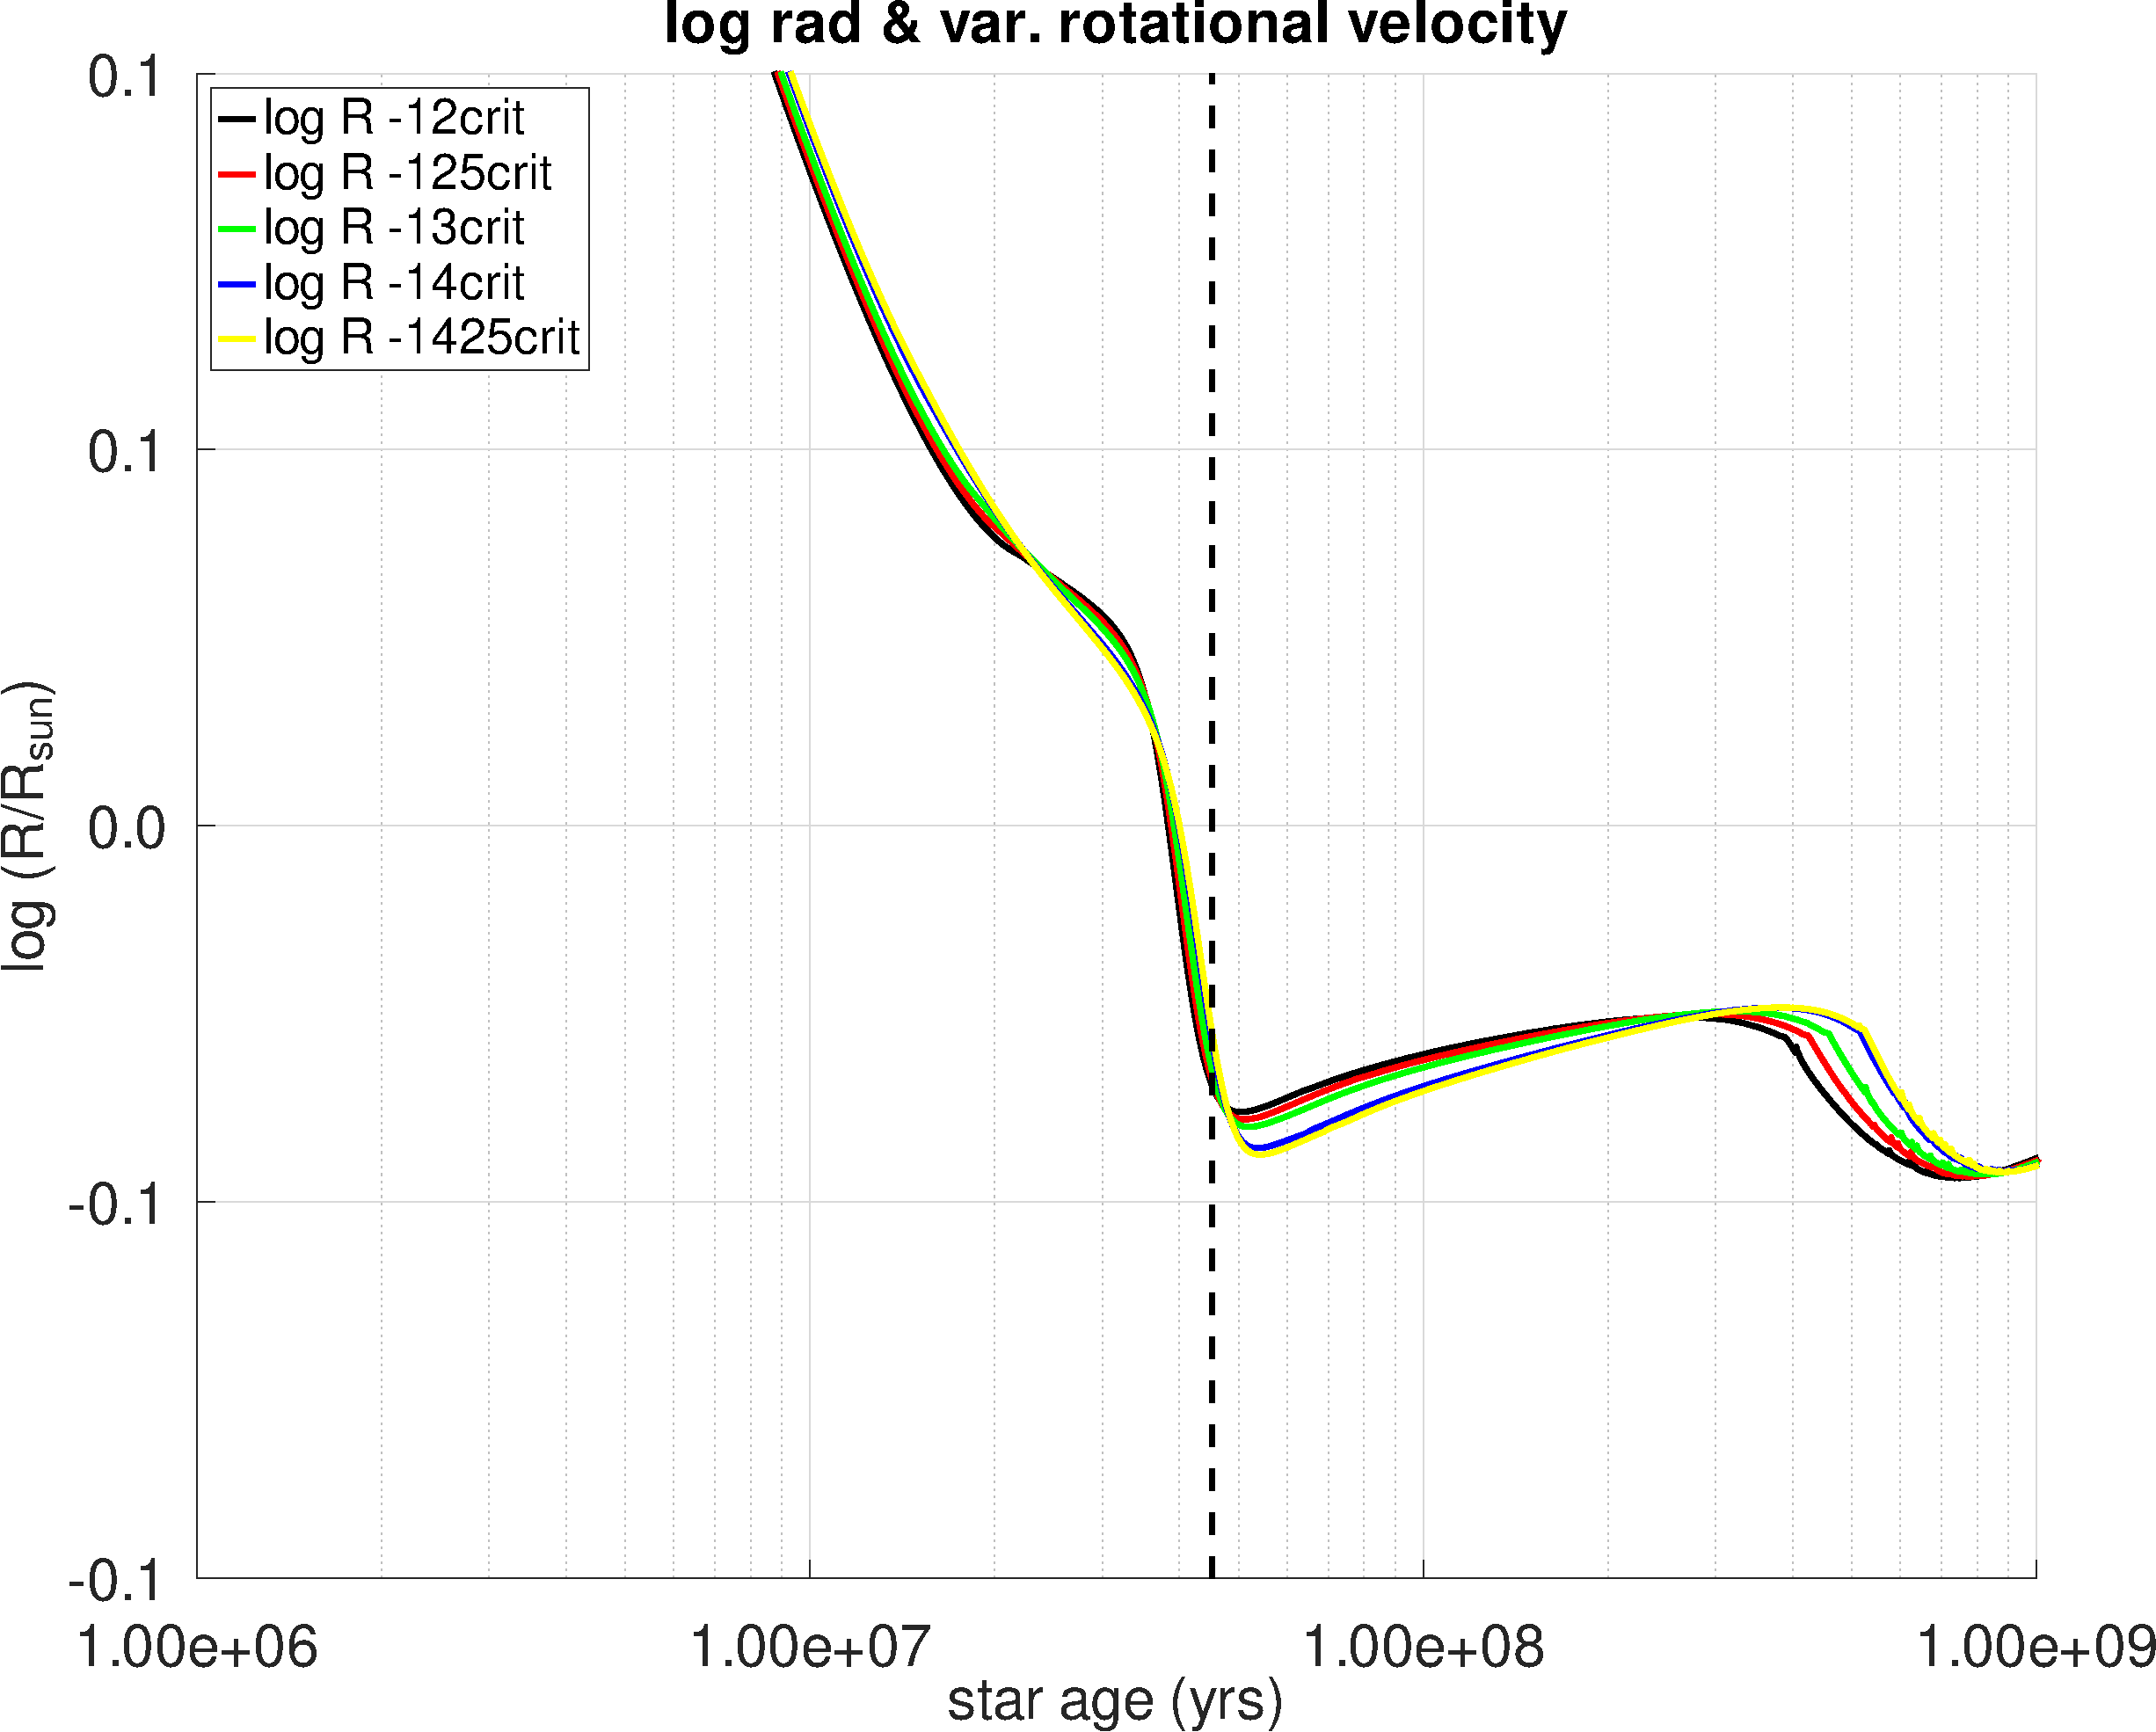
\includegraphics[clip,width=\columnwidth]{figures/paper2/lograd_var_vel_g_z13.pdf}
    \caption{Similar to Figure \ref{fig:lograd_var_vel_g3} but zooming in on the ZAMS. The fastest model exhibits the smallest radius from around $4.5x10^{7}$ till $11.0x10^{7}$ years.}
    \label{fig:lograd_var_vel_g_z13}
\end{figure}


\subsection{Gossage et al. (2021) Comparison}
In \cite{Gossage2021}, the authors also approach the problem of AML from a similar starting point to ours, but with some notable differences. In the Table \ref{tab:gassage_vs_navarro} we compare the most notable similarities and differences between the two studies. In both works the models consider rotation not only in the MS but also in the PMS, with the difference that in Gossage's work they take into account disk-locking. This aspect is not so important in our simulations since in our case we have focused on the A(Li) profiles. In contrast, Gossage's work focuses mainly on modelling rotation profiles of stars, which are significantly affected by disk-locking. Similarly, the effects of magnetic braking on angular momentum loss are also considered. In our case for stars with 1$\msun$ (solar-twins) and in their with 0.1$\msun$$\le$$\mstar$$\le$1.3$\msun$. Both models also use MLT but in our case the MLT alpha value is not pre-fixed but varies throughout the simulation. These two works complement each other as they are based on different formalisms. On the one hand, our work is based on the proposal of \cite{Gallet2013} whose most relevant parameters are Ro and the presence of a magnetic field of varying strength (B), and on the other hand Gossage presents two formalisms: \cite{Matt2015} and \cite{Garraffo2018}. The former is mainly characterised by $\rossby$ and the $\mstar$, while the latter by $\rossby$ and the complexity of the magnetic field ($\magfc$). As far as OCs observations are concerned, in this work we have had access to a larger number of them, and covered a wider range of ages [0.001-6.761] Gyr. Finally, both papers simulate their respective models in MESA.\par

\begin{table}
	\centering
	\caption{Comparison with \cite{Gossage2021} work.}
	\label{tab:gassage_vs_navarro}
        \begin{threeparttable}
	\begin{tabular}{lll} 
		\hline
		Parameter & This work & \cite{Gossage2021}\\
		\hline
            
		Rotation & At PMS \& MS & At PMS \& MS\\
  		Solar Mass & $\mstar$=1$\msun$ & 0.1$\msun$$\le$$\mstar$$\le$1.3$\msun$ \\
		Convection & MLT variable $\alpha_{{\rm MLT}}$ & MLT fixed $\alpha_{{\rm MLT}}$\\
		Magnetic Braking & \cite{Gallet2013} & \cite{Matt2015}, \\ Formalism & & \cite{Garraffo2018}\\
            Magnetic Braking & $\rossbystar$ \& $\bstar$ & $\rossbystar$ \& $\mstar$, \\ Parameters & & $\rossbystar$ \& $\magfc$\tnote{(1)}\\
		Magnetic Field & B(G) variable & Not used\\ Strength & & \\
            Disk locking & Not present & Present\\
            Number of OC's & 64 & 11 \\
            Source of data & GDR3.0 GES DR5.0 & Several works \\
            MESA version & r10398 & r11701\\
		\hline
	\end{tabular}
        \end{threeparttable}
        \begin{tablenotes}\footnotesize
        \item (1) Magnetic field complexity
        \end{tablenotes}
\end{table}


\section{Conclusions and future works} \label{sec_conclusions}
We have shown, through the different simulated stellar models, that the effects induced by the combination of both rotation and magnetic braking mechanisms offer a plausible way to reconcile the observational data with the theoretical models. We propose that this result could be achieved by a law of interdependence between $\Omega$ and $B$. In contrast to our previous work, these new models remove the restrictions of pre-setting initial and fixed values along their time evolution for the magnetic field strength and the $\amlt$ parameter. We cross-checked the model results with measurements obtained from the Gaia and GES mission for stars with similar characteristics to our Sun, focusing on their Li abundances.

Our models seem to suggest a lower limit to the surface Li abundances of 1.133 dex for Sun-like stars, value which is within the margin of error obtained for the Sun (1.1 $\pm$ 0.1 dex). On the other hand, they predict a higher angular velocity (4.72 km/s) than the Sun (2.0 km/s) so that they could burn more Li and finally reproduced the Sun Li existing reservoirs. Coupled with this higher angular velocity, strong magnetic fields developed, triggering an intensive magnetic braking that slowed its angular velocity but not enough to match the present $\Omega$ value of the Sun. In addition, it should be noted that our models fail to replicate the average magnetic field strength of the Sun.\par

As far as Li abundance and $\Omega$ are concerned, our models, while not exactly reproducing the values of the Sun, show promising results. Although we have shown how both an evolving magnetic field strength and, a MLT parametrization could produce results in line with the observations, we must analyse them results obtained with caution and not draw any premature conclusions. Nonetheless, we can draw the following finding from the present work:

\begin{enumerate}
    \item A magnetic field with varying intensity is a valid alternative to explain the rotational history of Sun-like stars.
    \item A variable $\amlt$ eliminates the need to pre-fix its value in advance for the entire evolution of the star.
    \item Our models seem to suggest a lower limit to the observations provided by Gaia and GES for solar sibling stars.
    \item The strength of the magnetic field regulates the size of the star's convection zone. The magnetic field has a direct implication on the rotational history of the star, and the speed with which the star rotates impacts the size of the convective zone.     
    \item Inclusion of the magnetic field leads to cooler models and lower Li depletion in the MS.
    \item Disk-locking during PMS seem to be also required for explaining Li abundances in young clusters.
\end{enumerate}

We would like to conclude with the following thoughts for the next steps. It is a fact that our models still destroy too much Li when comparing the produced Li abundances obtained with those from Gaia and GES. Taking as starting point that faster rotating stars destroy more Li, other mechanisms, in addition to magnetic braking, are necessary to explain the observational data. Among them, disk locking to the protostellar disk could contribute to counteract the acceleration of the star during PMS. Thus, we would have two braking mechanisms acting at different ages of the star. The disk locking would act during the PMS and the magnetic braking mainly during the MS. This approach would establish a self-regulating mechanism over the angular velocity of the star that would end up directly influencing the both Li evolution and the magnetic field strength. For the latter, lower intensities are expected which could finally converge with that of our Sun. On the other hand, a lower rotational speed also means less Li destruction for our models. One way to compensate for this lower Li remaining is to resort to over-shooting (see \cite{Navarro2020}) an effect that has not been simulated in our models. By activating this mechanism, we would allow the Li to be reached by bubbles of material hot enough to destroy it, thus contributing to decrease its abundance. Ideally, as we have done with $\amlt$, overshooting should not be introduced as a free parameter but dependent on other fundamental stellar parameters.\par


\section*{Acknowledgements}
We wish to acknowledge the generous work and help offered by the MESA and TOPCAT communities. Authors acknowledges funding support from Spanish public funds (including FEDER fonds) for research under projects ESP2017-87676-C5-2-R and ESP2017-87676-C5-5-R. JCS also acknowledges support from project RYC-2012-09913 under the 'Ram\'on y Cajal' program of the Spanish Ministry of Science and Education.

\section*{Software}
The simulations used in this paper been executed with the MESA release 10398 \footnote{\url{http://mesa.sourceforge.net/release/2018/03/21/r10398.html}}. The different figures have been generated making use of GNU Octave 5.1.0. \footnote{\url{https://www.gnu.org/software/octave/}}. The Gaia and GES data sets have been analyzed using TOPCAT 4.8-7 \footnote{\url{https://www.g-vo.org/topcat/topcat/}}. 

%%%%%%%%%%%%%%%%%%%%%%%%%%%%%%%%%%%%%%%%%%%%%%%%%%

%%%%%%%%%%%%%%%%%%%% REFERENCES %%%%%%%%%%%%%%%%%%

% The best way to enter references is to use BibTeX:

\bibliographystyle{mnras}
%\bibliography{magbrlitium} % if your bibtex file is called example.bib
\bibliography{mblithium}


% Alternatively you could enter them by hand, like this:
% This method is tedious and prone to error if you have lots of references
%\begin{thebibliography}{99}
%\bibitem[\protect\citeauthoryear{Author}{2012}]{Author2012}
%Author A.~N., 2013, Journal of Improbable Astronomy, 1, 1
%\bibitem[\protect\citeauthoryear{Others}{2013}]{Others2013}
%Others S., 2012, Journal of Interesting Stuff, 17, 198
%\end{thebibliography}

%%%%%%%%%%%%%%%%%%%%%%%%%%%%%%%%%%%%%%%%%%%%%%%%%%

%%%%%%%%%%%%%%%%% APPENDICES %%%%%%%%%%%%%%%%%%%%%
\appendix
\section{Full list of OC's}

\begin{table*}
	\centering
	\begin{tabular}{|l l l l l || c c c c c | c c c c c|} 
		\hline
             & & & & & & & $\oomegac$ & & & & & $\oomegac$ & & \\
		Open Cluster & GES\_FLD & Age (Gyr) & [Fe/H] & $N_*$ & 0.095 & 0.10 & 0.105 & 0.11 & 0.115 & 0.12 & 0.125 & 0.13 & 0.14 & 0.1425\\
		\hline
            25 Ori & 25\_Ori & 0.013 & 0 & 294 & 0 & 0 & 0 & 0 & 0 & 0 & 0 & 0 & 0 & 0\\
            ASCC 50 & Assc50 & 0.011 & 0.02 & 1225 & 0 & 0 & 0 & 0 & 0 & 0 & 0 & 0 & 0 & 0\\
            \rowcolor{lightgray}
            Berkeley 21 & Br21 & 2.138 & -0.21 & 744 & 0 & 0 & 0 & 0 & 0 & 1 & 1 & 1 & 1 & 1\\
            Berkeley 22 & Br22 & 2.455 & -0.26 & 395 & 0 & 0 & 0 & 0 & 0 & 0 & 0 & 0 & 0 & 0\\
            Berkeley 25 & Br25 & 2.455 & -0.25 & 81 & 0 & 0 & 0 & 0 & 0 & 0 & 0 & 0 & 0 & 0\\
            Berkeley 30 & Br30 & 0.295 & -0.13 & 332 & 0 & 0 & 0 & 0 & 0 & 0 & 0 & 0 & 0 & 0\\
            Berkeley 31 & Br31 & 2.818 & -0.29 & 616 & 0 & 0 & 0 & 0 & 0 & 0 & 0 & 0 & 0 & 0\\
            Berkeley 32 & Br32 & 4.898 & -0.31 & 438 & 0 & 0 & 0 & 0 & 0 & 0 & 0 & 0 & 0 & 0\\
            Berkeley 36 & Br36 & 6.761 & -0.15 & 739 & 0 & 0 & 0 & 0 & 0 & 0 & 0 & 0 & 0 & 0\\
            \rowcolor{lightgray}
            Berkeley 39 & Br39 & 5.623 & -0.14 & 899 & 1 & 1 & 1 & 1 & 1 & 1 & 2 & 2 & 2 & 2\\
            Berkeley 44 & Br44 & 1.445 & 0.22 & 93 & 0 & 0 & 0 & 0 & 0 & 0 & 0 & 0 & 0 & 0\\
            Berkeley 73 & Br73 & 1.413 & -0.26 & 77 & 0 & 0 & 0 & 0 & 0 & 0 & 0 & 0 & 0 & 0\\
            Berkeley 75 & Br75 & 1.738 & -0.34 & 75 & 0 & 0 & 0 & 0 & 0 & 0 & 0 & 0 & 0 & 0\\
            Berkeley 81 & Br81 & 1.148 & 0.22 & 279 & 0 & 0 & 0 & 0 & 0 & 0 & 0 & 0 & 0 & 0\\
            Blanco 1 & Blanco1 & 0.105 & -0.03 & 463 & 0 & 0 & 0 & 0 & 0 & 0 & 0 & 0 & 0 & 0\\
            Chamaeleon I & Cha\_I & 0.001 & -0.03 & 709 & 0 & 0 & 0 & 0 & 0 & 0 & 0 & 0 & 0 & 0\\
            Collinder 197 & Col197 & 0.014 & 0.03 & 409 & 0 & 0 & 0 & 0 & 0 & 0 & 0 & 0 & 0 & 0\\
            Collinder 69 & lam\_Ori & 0.013 & -0.09 & 836 & 0 & 0 & 0 & 0 & 0 & 0 & 0 & 0 & 0 & 0\\
            Czernik 24 & Cz24 & 2.692 & -0.11 & 346 & 0 & 0 & 0 & 0 & 0 & 0 & 0 & 0 & 0 & 0\\
            Czernik 30 & Cz30 & 2.884 & -0.31 & 226 & 0 & 0 & 0 & 0 & 0 & 0 & 0 & 0 & 0 & 0\\
            ESO 92-05 & ESO92\_05 & 4.467 & -0.29 & 212 & 0 & 0 & 0 & 0 & 0 & 0 & 0 & 0 & 0 & 0\\
            Haffner 10 & Haf10 & 3.802 & -0.1 & 562 & 0 & 0 & 0 & 0 & 0 & 0 & 0 & 0 & 0 & 0\\
            IC 2391 & IC2391 & 0.029 & -0.06 & 434 & 0 & 0 & 0 & 0 & 0 & 0 & 0 & 0 & 0 & 0\\
            \rowcolor{lightgray}
            IC 2602 & IC2602 & 0.036 & -0.06 & 1836 & 0 & 0 & 0 & 0 & 0 & 0 & 1 & 1 & 0 & 0\\
            \rowcolor{lightgray}
            IC 4665 & IC4665 & 0.033 & 0.01 & 567 & 0 & 0 & 0 & 0 & 1 & 1 & 0 & 0 & 0 & 0\\
            Loden 165 & Loden165 & 3 &  & 388 & 0 & 0 & 0 & 0 & 0 & 0 & 0 & 0 & 0 & 0\\
            \rowcolor{lightgray}
            Messier 67 & M67 & 3.981 & -0.02 & 131 & 6 & 6 & 6 & 6 & 6 & 6 & 6 & 6 & 6 & 6\\
            \rowcolor{lightgray}
            NGC 2141 & NGC2141 & 1.862 & -0.04 & 853 & 1 & 1 & 1 & 1 & 1 & 1 & 1 & 1 & 1 & 1\\
            NGC 2158 & NGC2158 & 1.549 & -0.15 & 616 & 0 & 0 & 0 & 0 & 0 & 0 & 0 & 0 & 0 & 0\\
            NGC 2232 & NGC2232 & 0.018 & -0.03 & 1866 & 0 & 0 & 0 & 0 & 0 & 0 & 0 & 0 & 0 & 0\\
            NGC 2243 & NGC2243 & 4.365 & -0.45 & 661 & 0 & 0 & 0 & 0 & 0 & 0 & 0 & 0 & 0 & 0\\
            NGC 2244 & NGC2244 & 0.004 & -0.04 & 452 & 0 & 0 & 0 & 0 & 0 & 0 & 0 & 0 & 0 & 0\\
            NGC 2264 & NGC2264 & 0.003 & -0.1 & 1857 & 0 & 0 & 0 & 0 & 0 & 0 & 0 & 0 & 0 & 0\\
            \rowcolor{lightgray}
            NGC 2355 & NGC2355 & 1 & -0.13 & 208 & 1 & 1 & 1 & 1 & 1 & 1 & 1 & 1 & 1 & 1\\
            \rowcolor{lightgray}
            NGC 2420 & NGC2420 & 1.698 & -0.15 & 562 & 1 & 1 & 1 & 1 & 1 & 1 & 1 & 1 & 1 & 1\\
            \rowcolor{lightgray}
            NGC 2425 & NGC2425 & 2.399 & -0.13 & 528 & 1 & 1 & 1 & 1 & 1 & 1 & 1 & 1 & 1 & 1\\
            \rowcolor{lightgray}
            NGC 2451 & NGC2451 & 0.035 & -0.08 & 1656 & 0 & 0 & 0 & 0 & 0 & 1 & 1 & 0 & 2 & 1\\
            \rowcolor{lightgray}
            NGC 2516 & NGC2516 & 0.24 & -0.04 & 759 & 0 & 0 & 0 & 1 & 1 & 1 & 3 & 4 & 4 & 3\\
            NGC 2547 & NGC2457 & 0.032 & -0.03 & 477 & 0 & 0 & 0 & 0 & 0 & 0 & 0 & 0 & 0 & 0\\
            NGC 3293 & NGC3293 & 0.01 & -0.08 & 584 & 0 & 0 & 0 & 0 & 0 & 0 & 0 & 0 & 0 & 0\\
            \rowcolor{lightgray}
            NGC 3532 & NGC3532 & 0.398 & -0.01 & 1145 & 1 & 1 & 0 & 1 & 1 & 1 & 1 & 1 & 0 & 1\\
            NGC 3766 & NGC3766 & 0.023 & -0.12 & 399 & 0 & 0 & 0 & 0 & 0 & 0 & 0 & 0 & 0 & 0\\
            NGC 4815 & NGC4815 & 0.372 & 0.08 & 218 & 0 & 0 & 0 & 0 & 0 & 0 & 0 & 0 & 0 & 0\\
            \rowcolor{lightgray}
            NGC 6005 & NGC6005 & 1.259 & 0.22 & 560 & 0 & 0 & 0 & 0 & 0 & 0 & 0 & 1 & 1 & 1\\
            NGC 6067 & NGC6067 & 0.126 & 0.03 & 780 & 0 & 0 & 0 & 0 & 0 & 0 & 0 & 0 & 0 & 0\\
            NGC 6253 & NGC6253 & 3.246 & 0.33 & 646 & 0 & 0 & 0 & 0 & 0 & 0 & 0 & 0 & 0 & 0\\
            \rowcolor{lightgray}
            NGC 6259 & NGC6259 & 0.269 & 0.18 & 494 & 0 & 0 & 0 & 0 & 0 & 0 & 0 & 0 & 0 & 1\\
            \rowcolor{lightgray}
            NGC 6281 & NGC6281 & 0.513 & -0.04 & 320 & 0 & 0 & 0 & 0 & 0 & 0 & 0 & 0 & 1 & 1\\
            \rowcolor{lightgray}
            NGC 6405 & NGC6405 & 0.035 & -0.02 & 701 & 1 & 1 & 1 & 0 & 1 & 3 & 2 & 0 & 0 & 0\\
            NGC 6530 & NGC6530 & 0.002 & -0.02 & 1983 & 0 & 0 & 0 & 0 & 0 & 0 & 0 & 0 & 0 & 0\\
            \rowcolor{lightgray}
            NGC 6633 & NGC6633 & 0.692 & -0.03 & 1662 & 2 & 2 & 2 & 1 & 1 & 0 & 0 & 0 & 1 & 1\\
            NGC 6649 & NGC6649 & 0.071 & -0.08 & 283 & 0 & 0 & 0 & 0 & 0 & 0 & 0 & 0 & 0 & 0\\
            NGC 6705 & NGC6705 & 0.309 & 0.03 & 1066 & 0 & 0 & 0 & 0 & 0 & 0 & 0 & 0 & 0 & 0\\
            \rowcolor{lightgray}
            NGC 6709 & NGC6709 & 0.191 & -0.02 & 730 & 2 & 1 & 0 & 0 & 0 & 0 & 0 & 0 & 1 & 1\\
            NGC 6802 & NGC6802 & 0.661 & 0.14 & 197 & 0 & 0 & 0 & 0 & 0 & 0 & 0 & 0 & 0 & 0\\
            Pismis 15 & Pismis15 & 0.871 & 0.02 & 333 & 0 & 0 & 0 & 0 & 0 & 0 & 0 & 0 & 0 & 0\\
            Pismis 18 & Pismis18 & 0.575 & 0.14 & 142 & 0 & 0 & 0 & 0 & 0 & 0 & 0 & 0 & 0 & 0\\
            Ruprecht 134 & Rup134 & 1.66 & 0.27 & 680 & 0 & 0 & 0 & 0 & 0 & 0 & 0 & 0 & 0 & 0\\
            Trumpler 14 & Trumpler14 & 0.003 & -0.01 & 1902 & 0 & 0 & 0 & 0 & 0 & 0 & 0 & 0 & 0 & 0\\
            \rowcolor{lightgray}
            Trumpler 20 & Trumpler20 & 1.862 & 0.13 & 1213 & 3 & 3 & 3 & 2 & 2 & 2 & 2 & 2 & 2 & 2\\
            Trumpler 23 & Trumpler23 & 0.708 & 0.2 & 165 & 0 & 0 & 0 & 0 & 0 & 0 & 0 & 0 & 0 & 0\\
            Trumpler 5 & Trumpler5 & 4.266 & -0.35 & 1138 & 0 & 0 & 0 & 0 & 0 & 0 & 0 & 0 & 0 & 0\\
            Gamma Vel & gamma2\_vel & 0.02 & -0.02 & 1269 & 0 & 0 & 0 & 0 & 0 & 0 & 0 & 0 & 0 & 0\\
            Rho Oph & Rho\_Oph & 0.001 & 0.03 & 311 & 0 & 0 & 0 & 0 & 0 & 0 & 0 & 0 & 0 & 0\\           
            \hline
	\end{tabular}
 	\caption{List of selected OCs. For each OC, name, GES denomination, estimated age, metallicity and number of components are listed. The number of OC components selected by the different simulations are shown separately. This information is split into two groups, each corresponding to the set of simulations used in the figures shown in the following sections. Finally, those OCs that have been selected in any of the simulations are highlighted in grey.}
  	\label{tab:oc_full_list}
\end{table*}


\clearpage
\section{Grid models visualization}
The following figures comprise a series of grids as a function of time and for several 1 $\msun$ models in which on the one hand, the evolution of surface \isotope[7]{Li} abundance relative to \isotope[1]{H} for both variable magnetic field intensities and angular velocities and on the other hand, the evolution of surface rotational velocity are shown.

\begin{figure*}
    \centering
    \begin{subfigure}[h]{0.47\textwidth}
    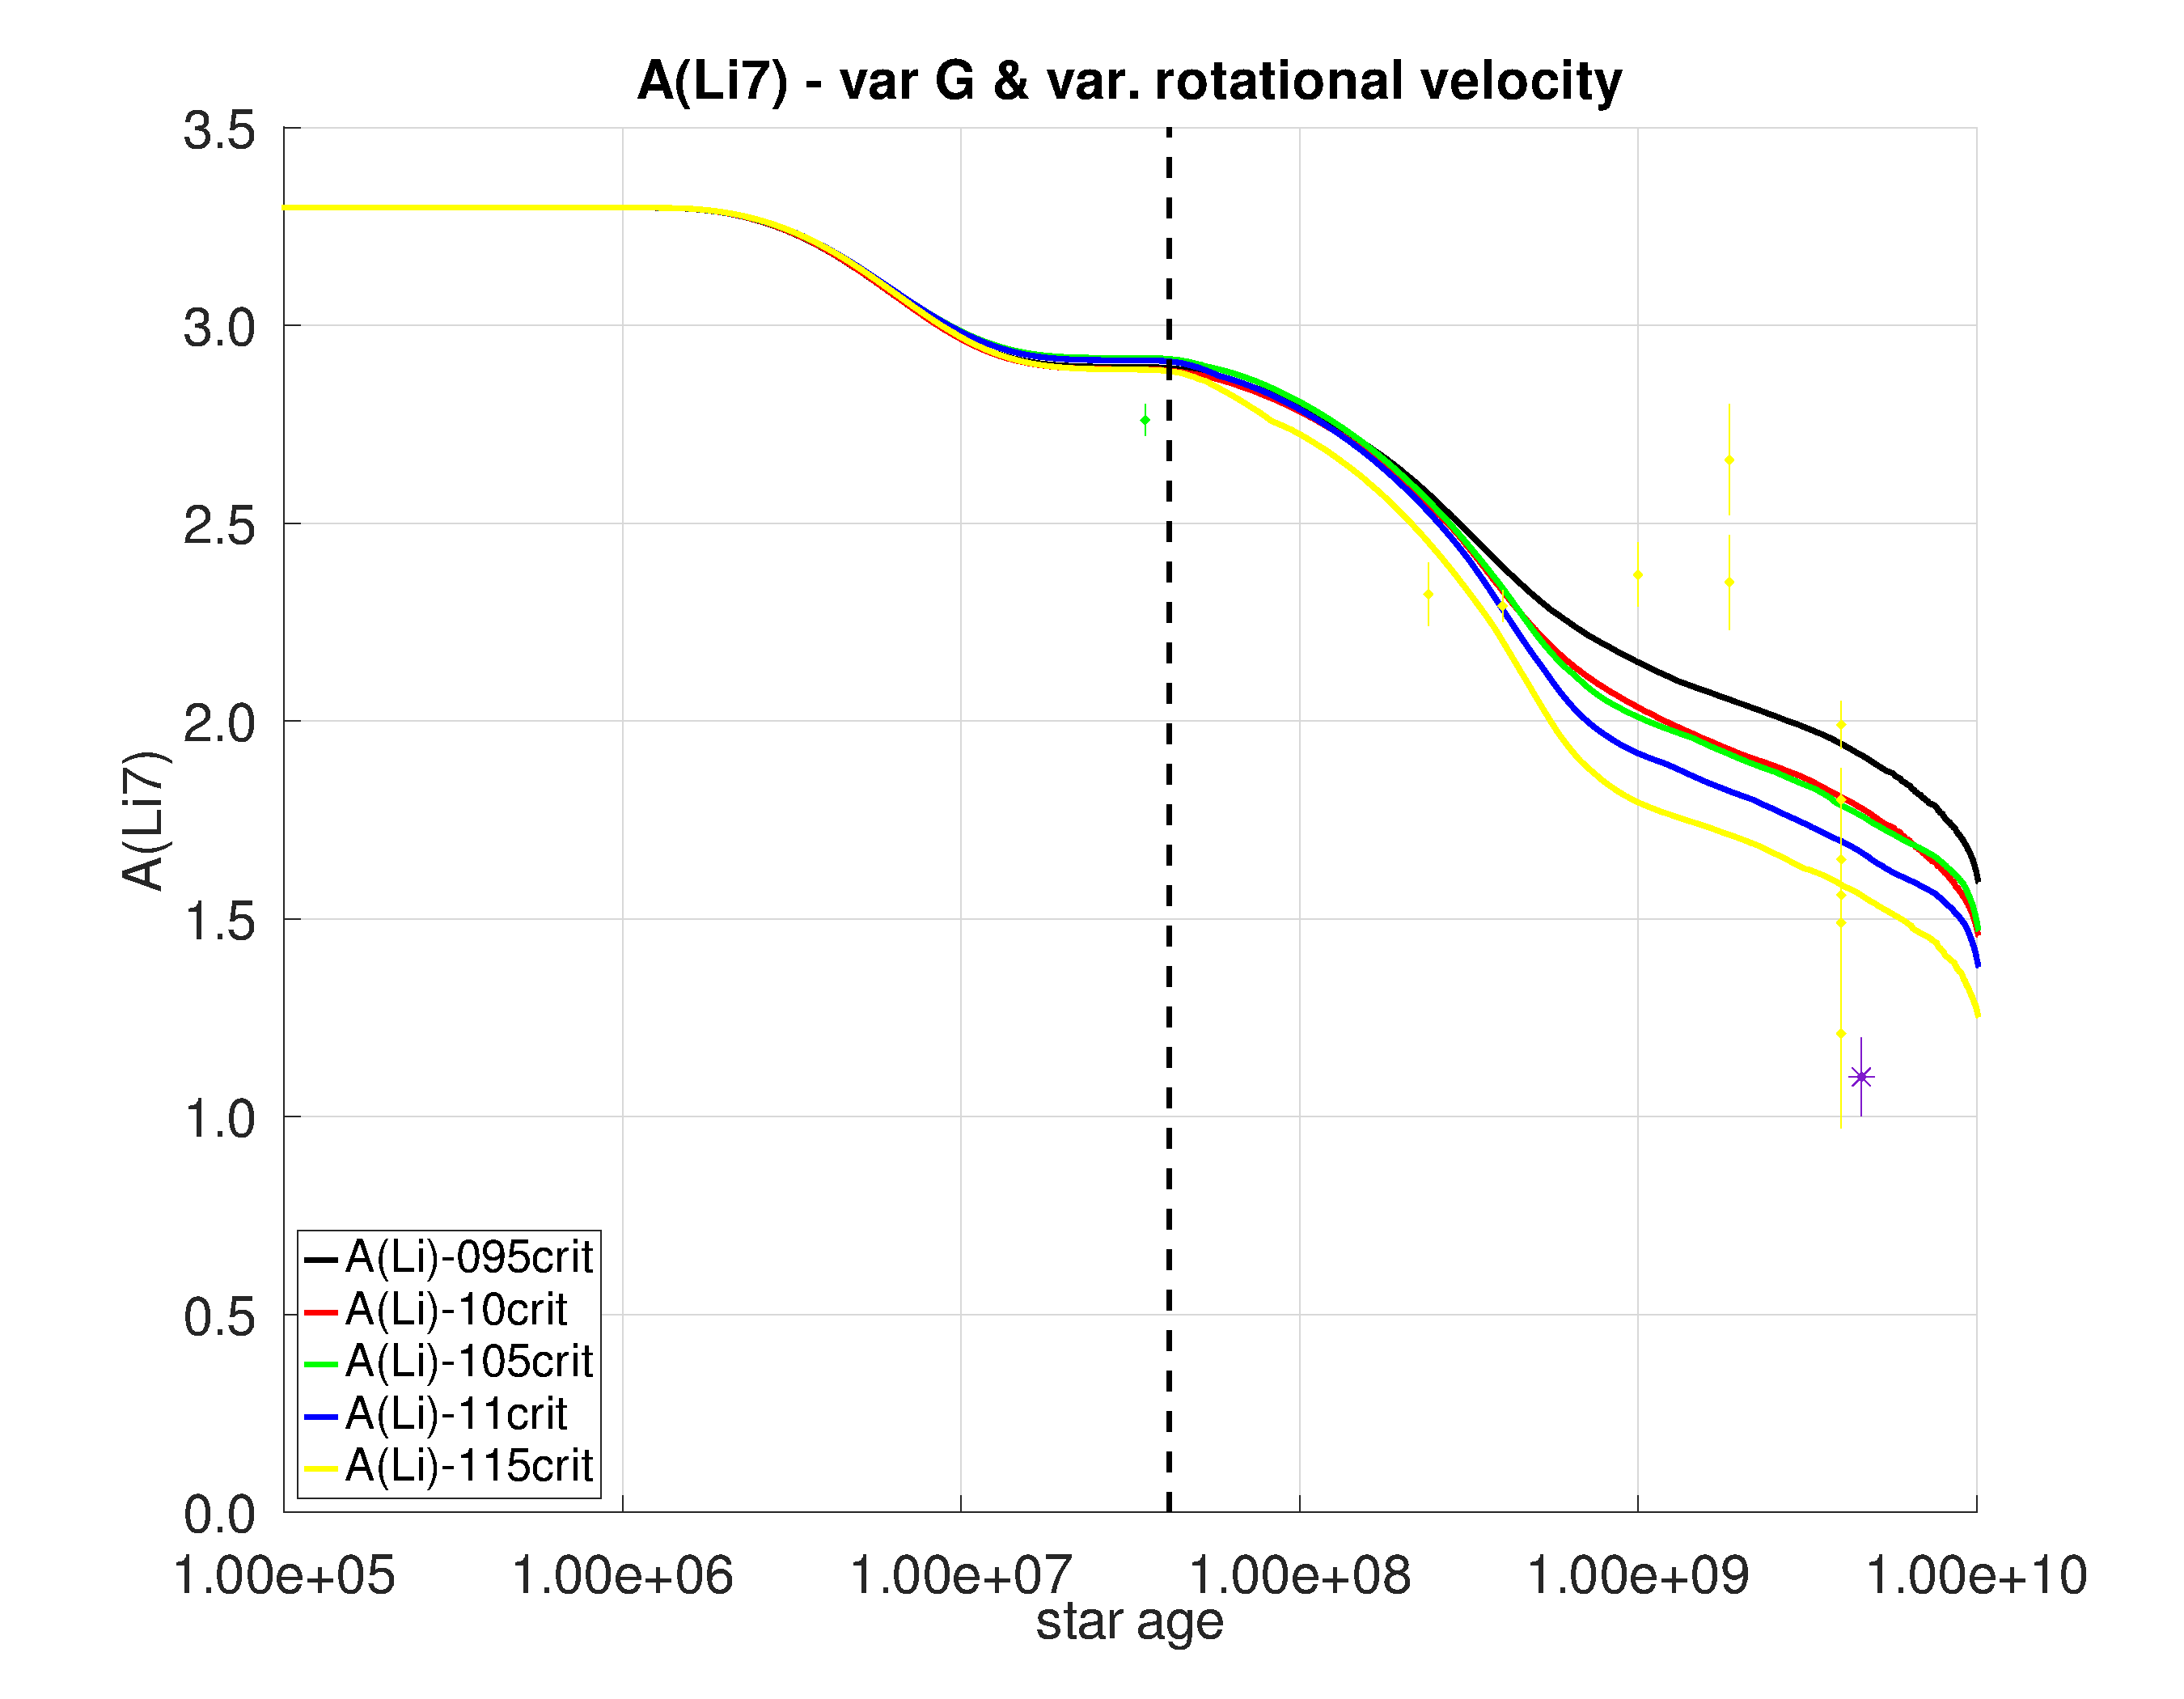
\includegraphics[clip,width=\textwidth]{figures/paper2/li_var_vel_var_g_1.pdf}
    \label{fig:subim11}
    \end{subfigure}
    \begin{subfigure}[h]{0.47\textwidth}
    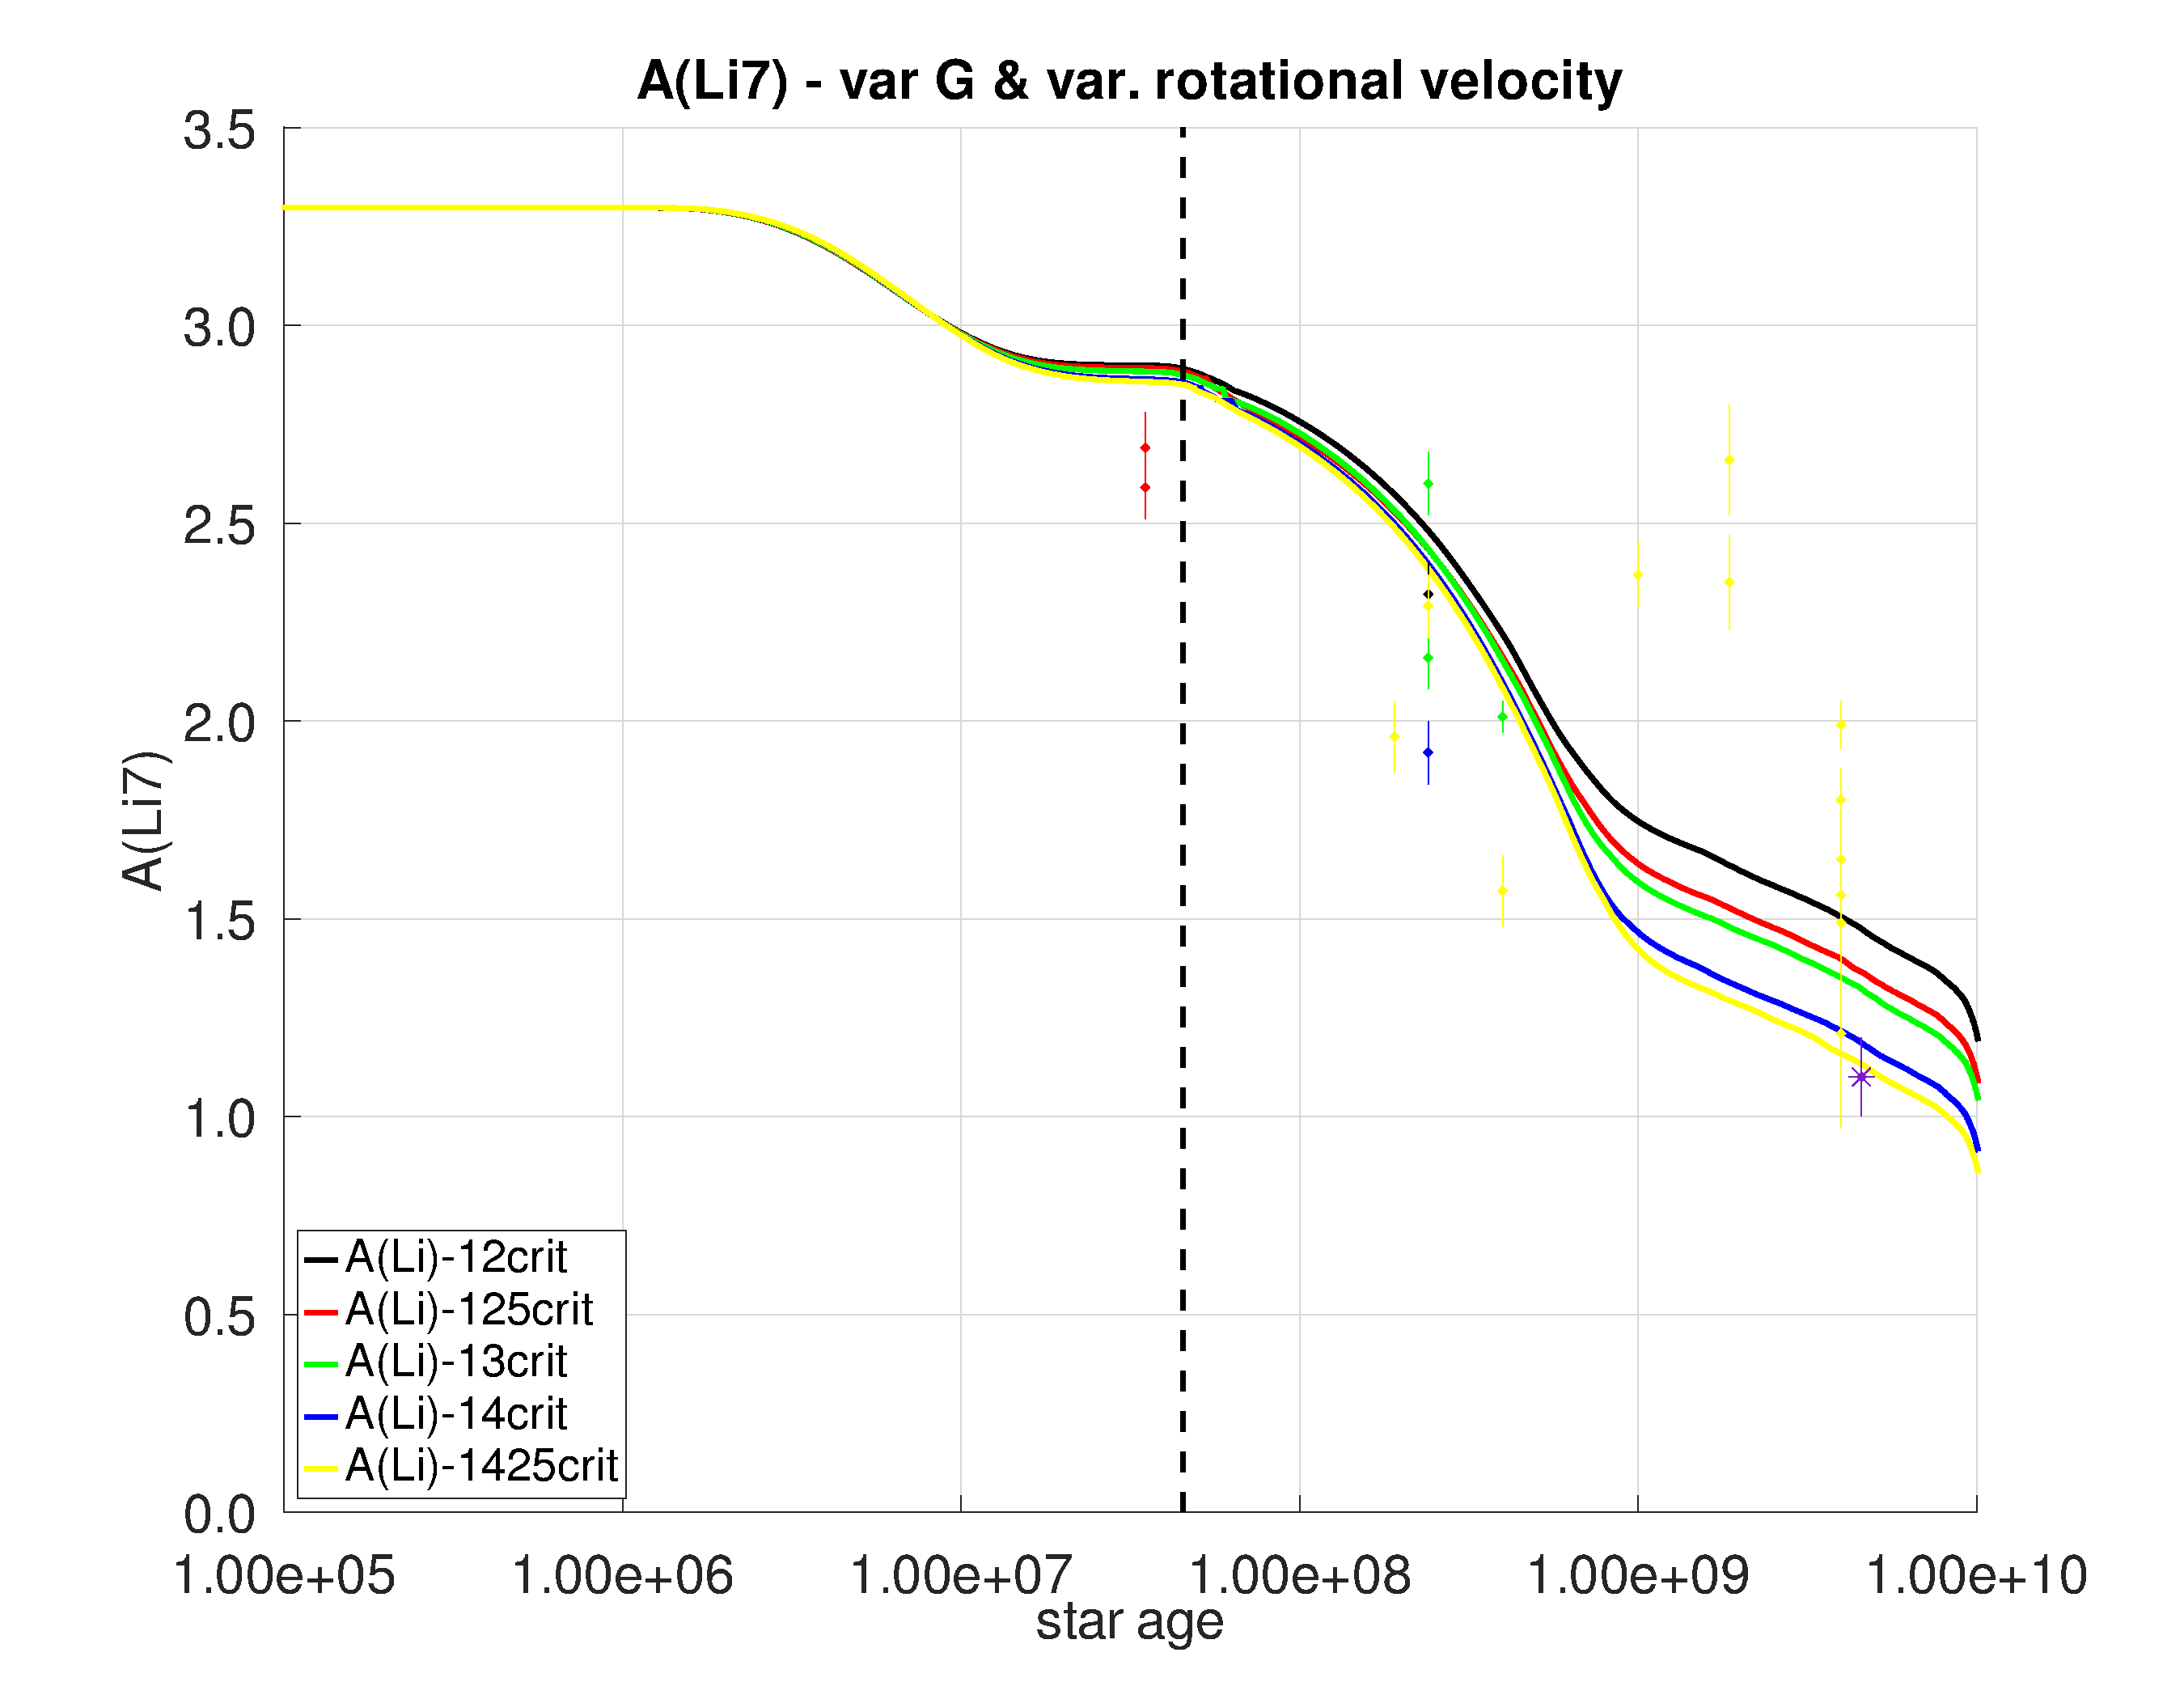
\includegraphics[clip,width=\textwidth]{figures/paper2/li_var_vel_var_g_3.pdf}
    \label{fig:subim12}
    \end{subfigure}
    \begin{subfigure}[h]{0.47\textwidth}
    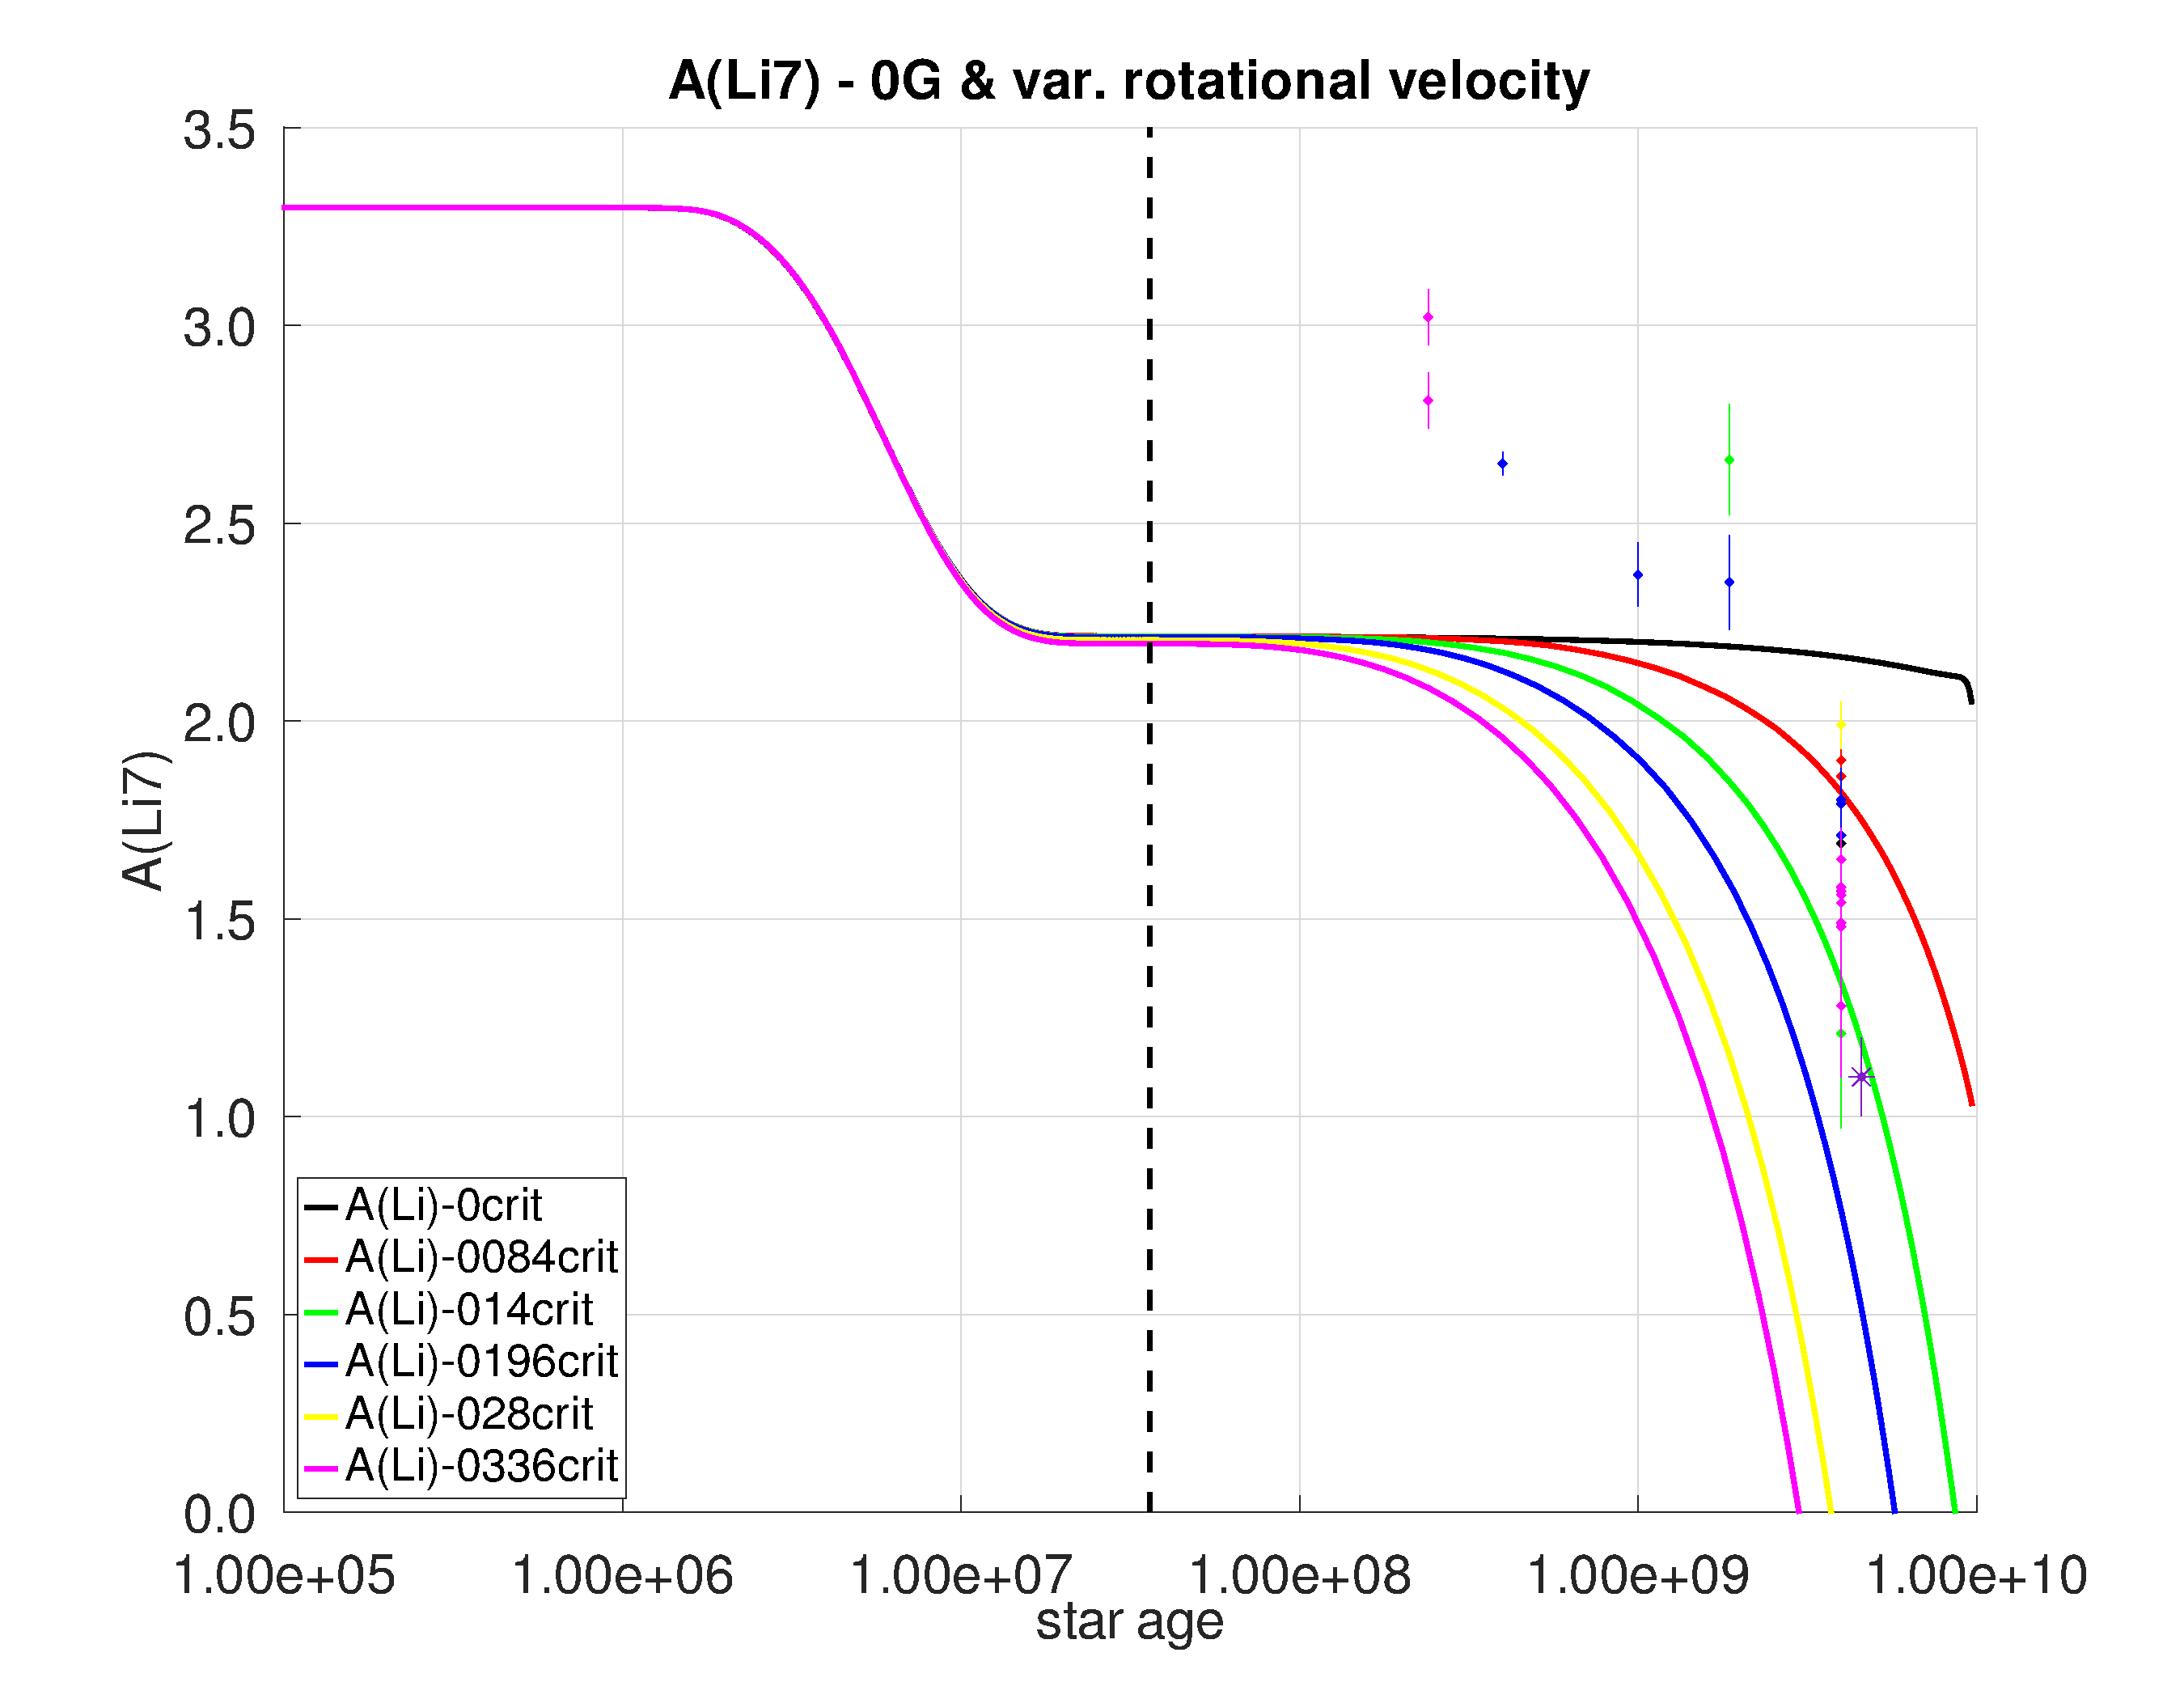
\includegraphics[trim = 25mm 10mm 15mm 10mm, clip,width=\textwidth]{figures/paper2/li_var_vel_0_0g_0.pdf}
    \label{fig:subim13}
    \end{subfigure}
    \begin{subfigure}[h]{0.47\textwidth}
    
\includegraphics[width=\textwidth]{figures/blank.eps}
    \label{fig:subim14}
    \end{subfigure}

\caption{Grid showing the evolution of surface \isotope[7]{Li} abundance relative to \isotope[1]{H}, as a function of time for several 1 $\msun$ models. Each figure shows a set of models in which the magnetic field with intensity has been fixed and $\oomegac$ varies between 0.0084 and 0.0336, respectively. The purple star and square are surface Li abundance for the present-day Sun \citep{Asplund2009} and the Pleiades cluster \citep{Sestito2005} respectively. The dashed vertical line makes reference to the ZAMS.}
\label{fig:grid_li_var_vel}
\end{figure*}
\par


\begin{figure*}
    \centering
    \begin{subfigure}[h]{0.47\textwidth}
    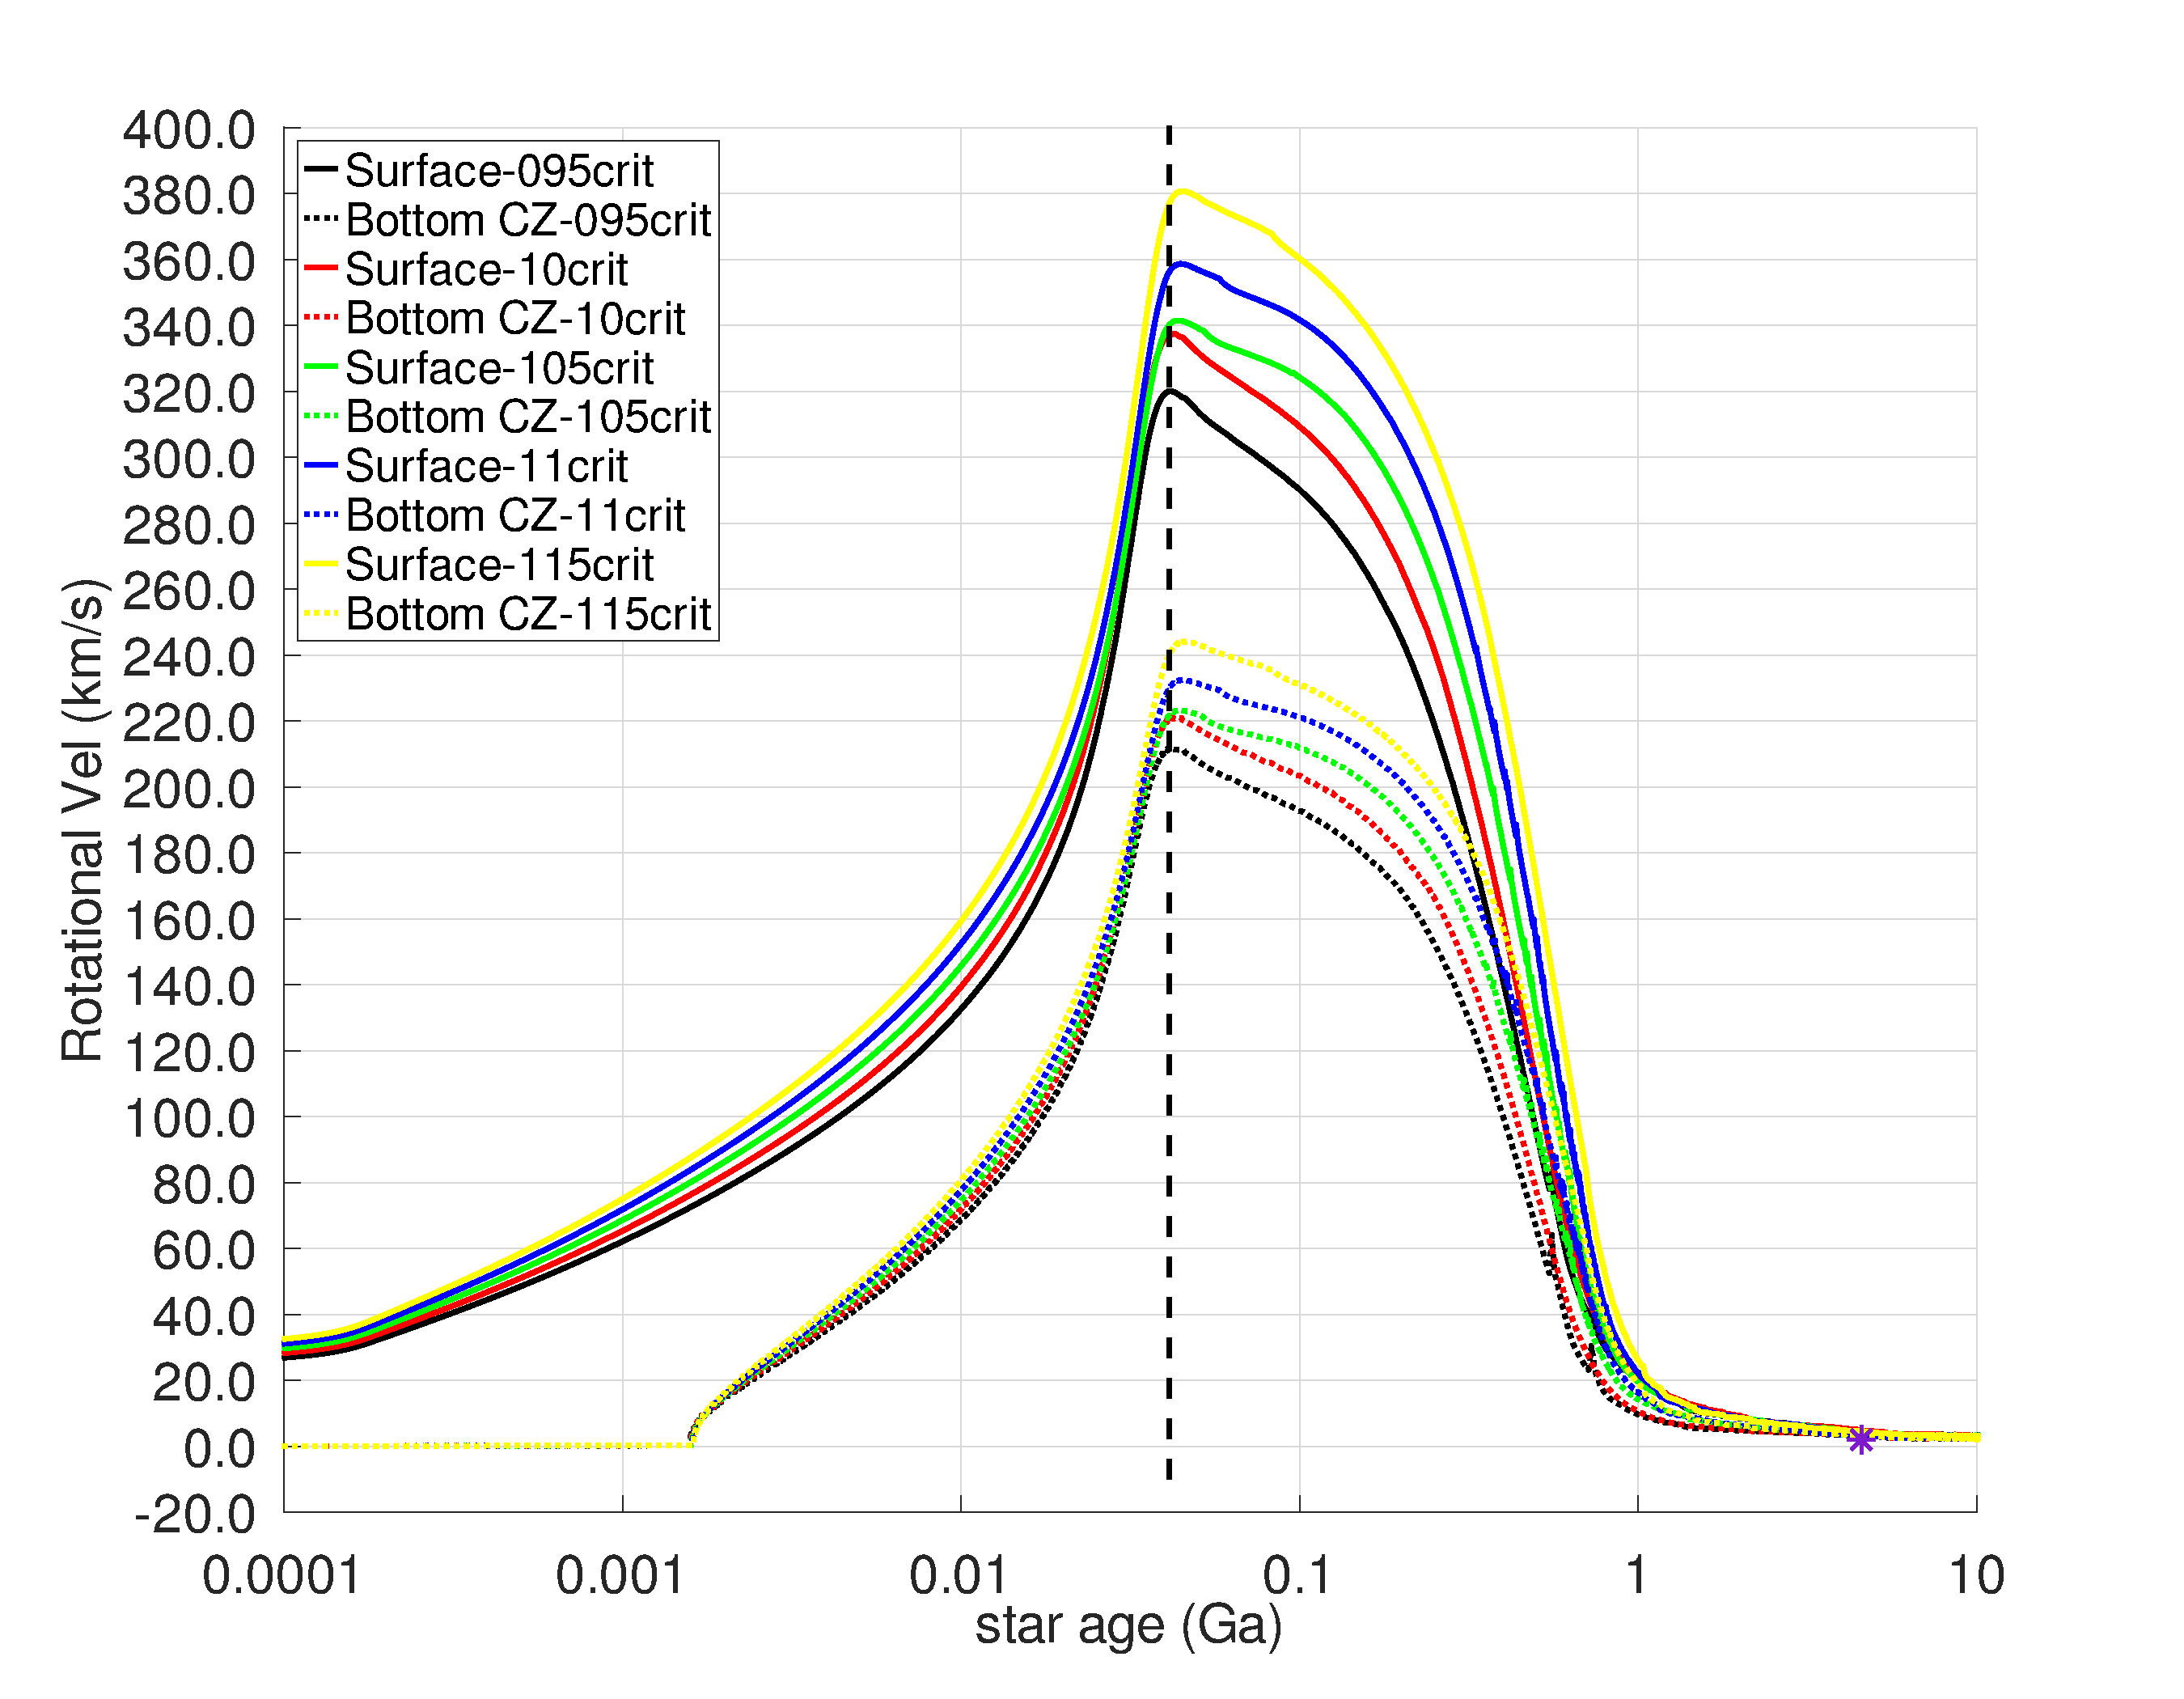
\includegraphics[clip,width=\textwidth]{figures/paper2/rot_vel_var_vel_var_g1.pdf}
    \label{fig:subim21}
    \end{subfigure}
    \begin{subfigure}[h]{0.47\textwidth}
    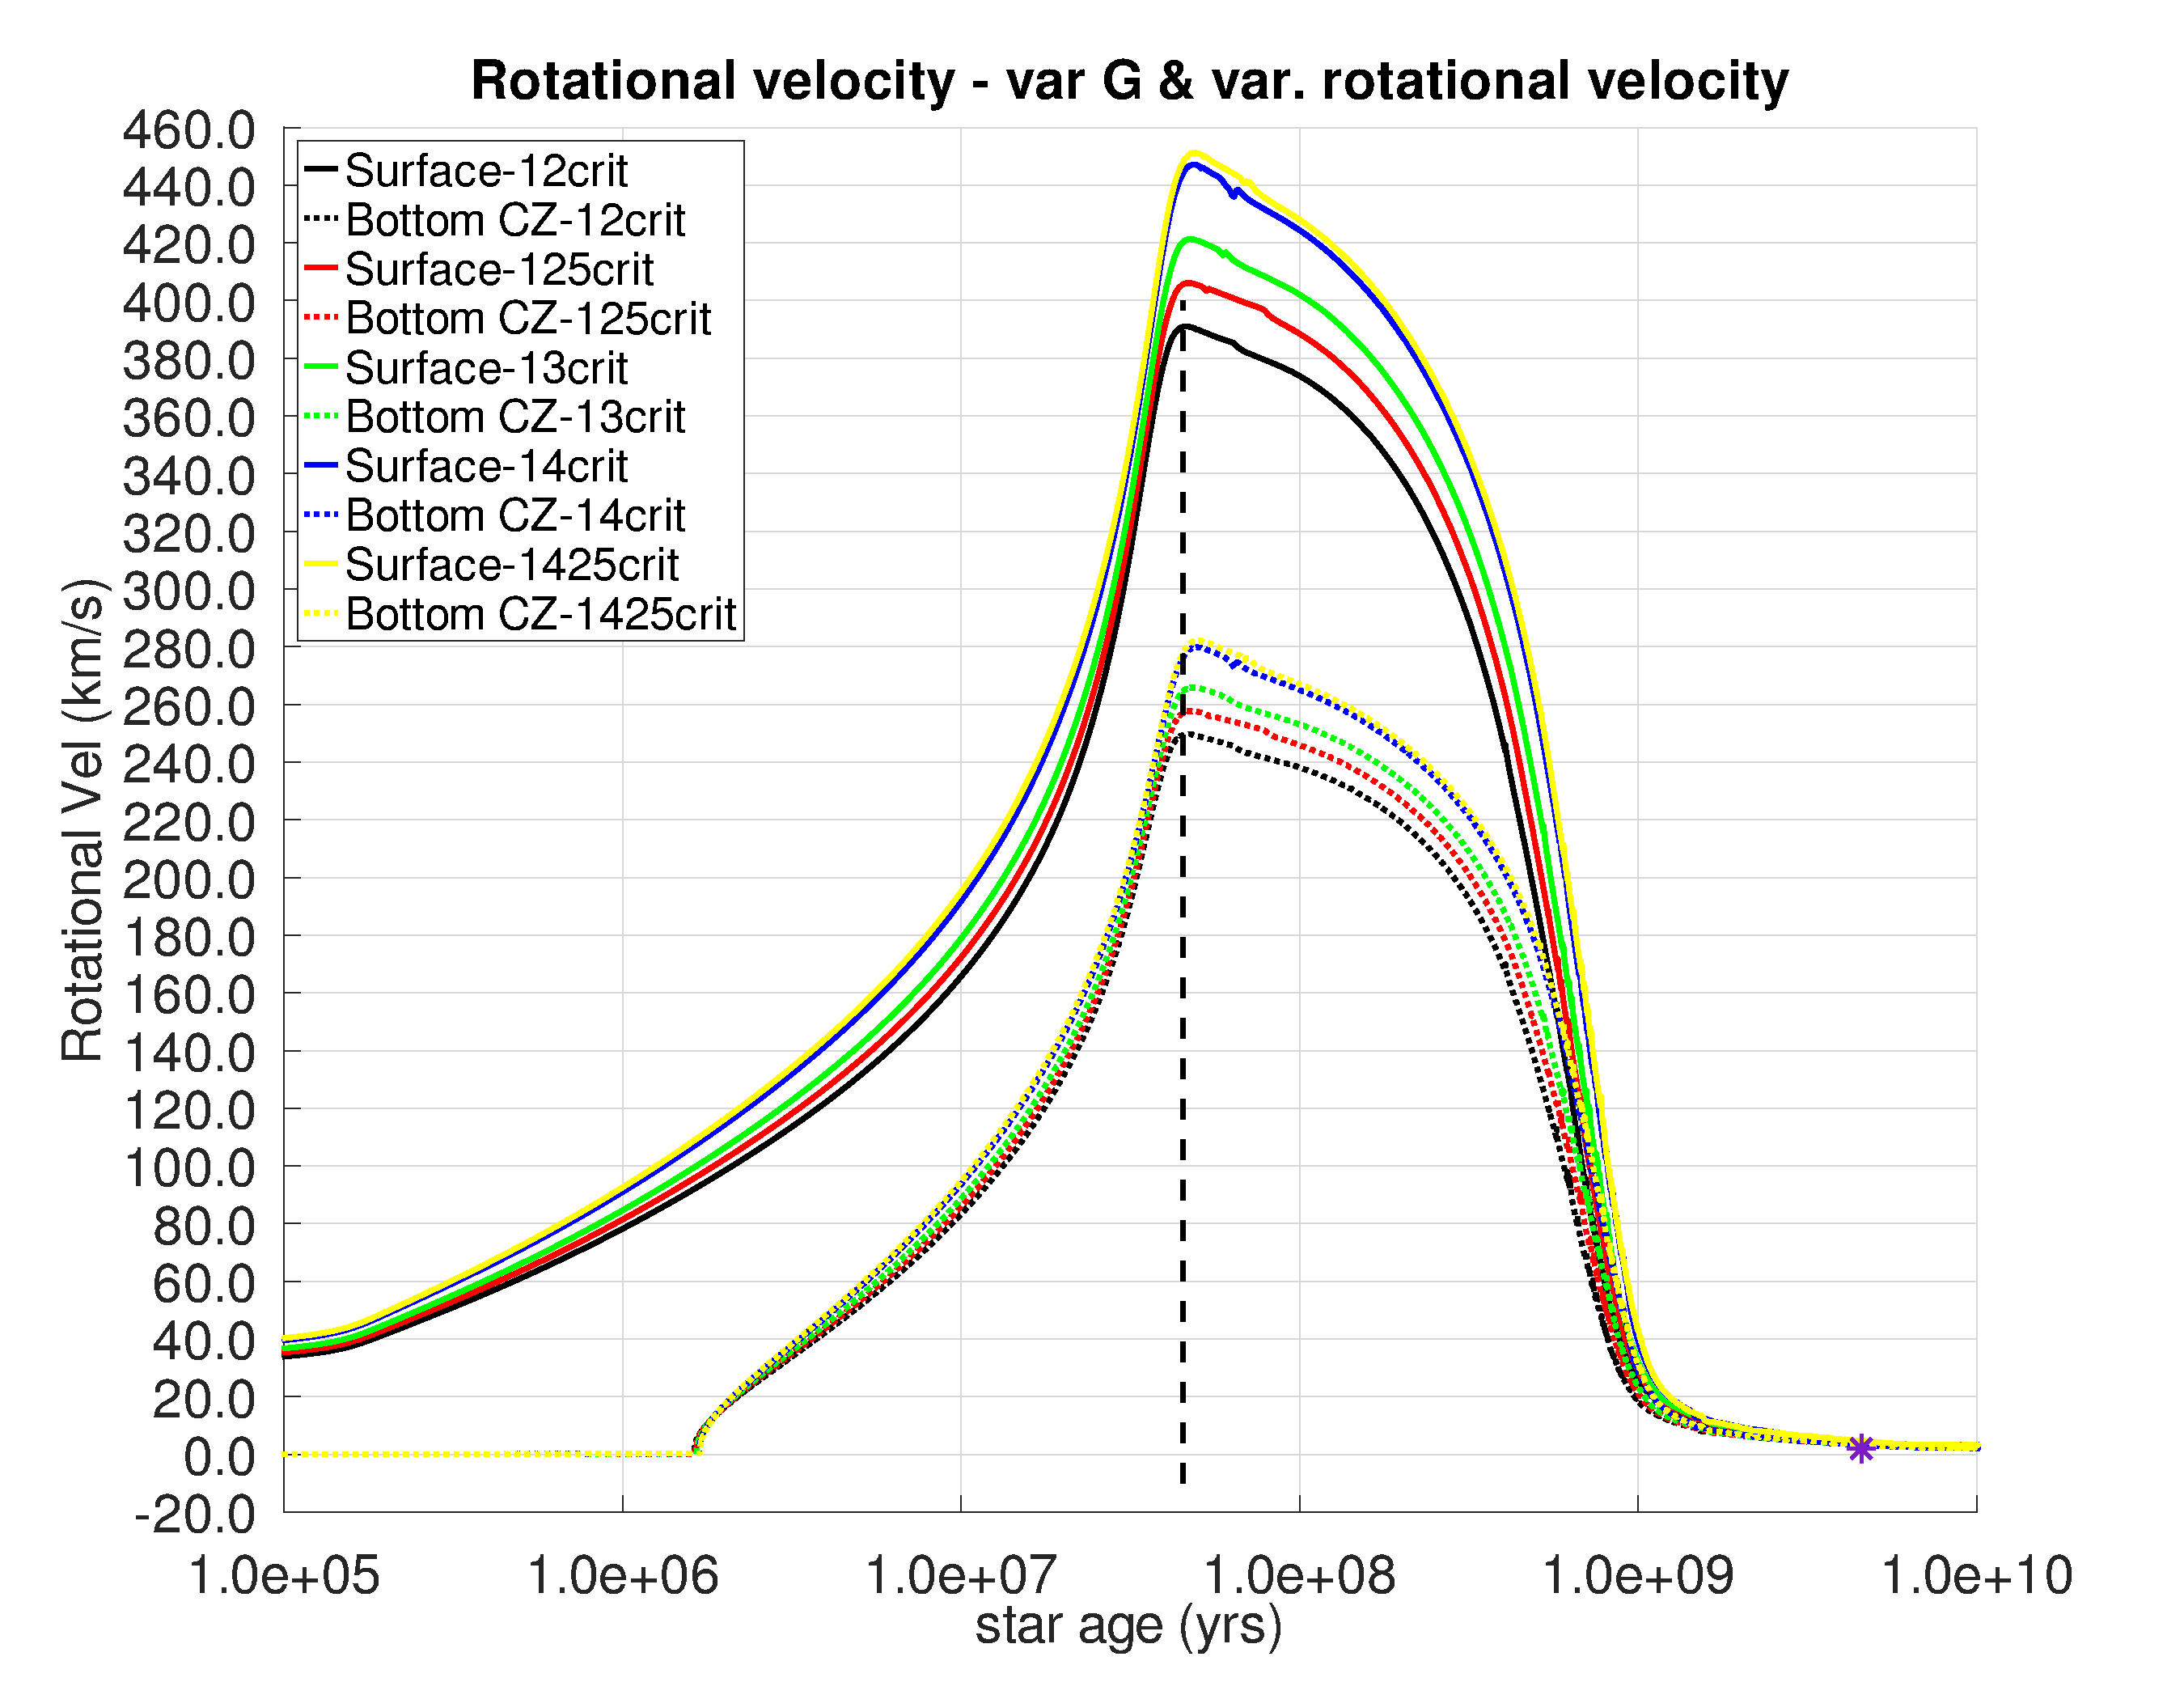
\includegraphics[clip,width=\textwidth]{figures/paper2/rot_vel_var_vel_var_g3.pdf}
    \label{fig:subim22}
    \end{subfigure}
    \begin{subfigure}[h]{0.47\textwidth}
    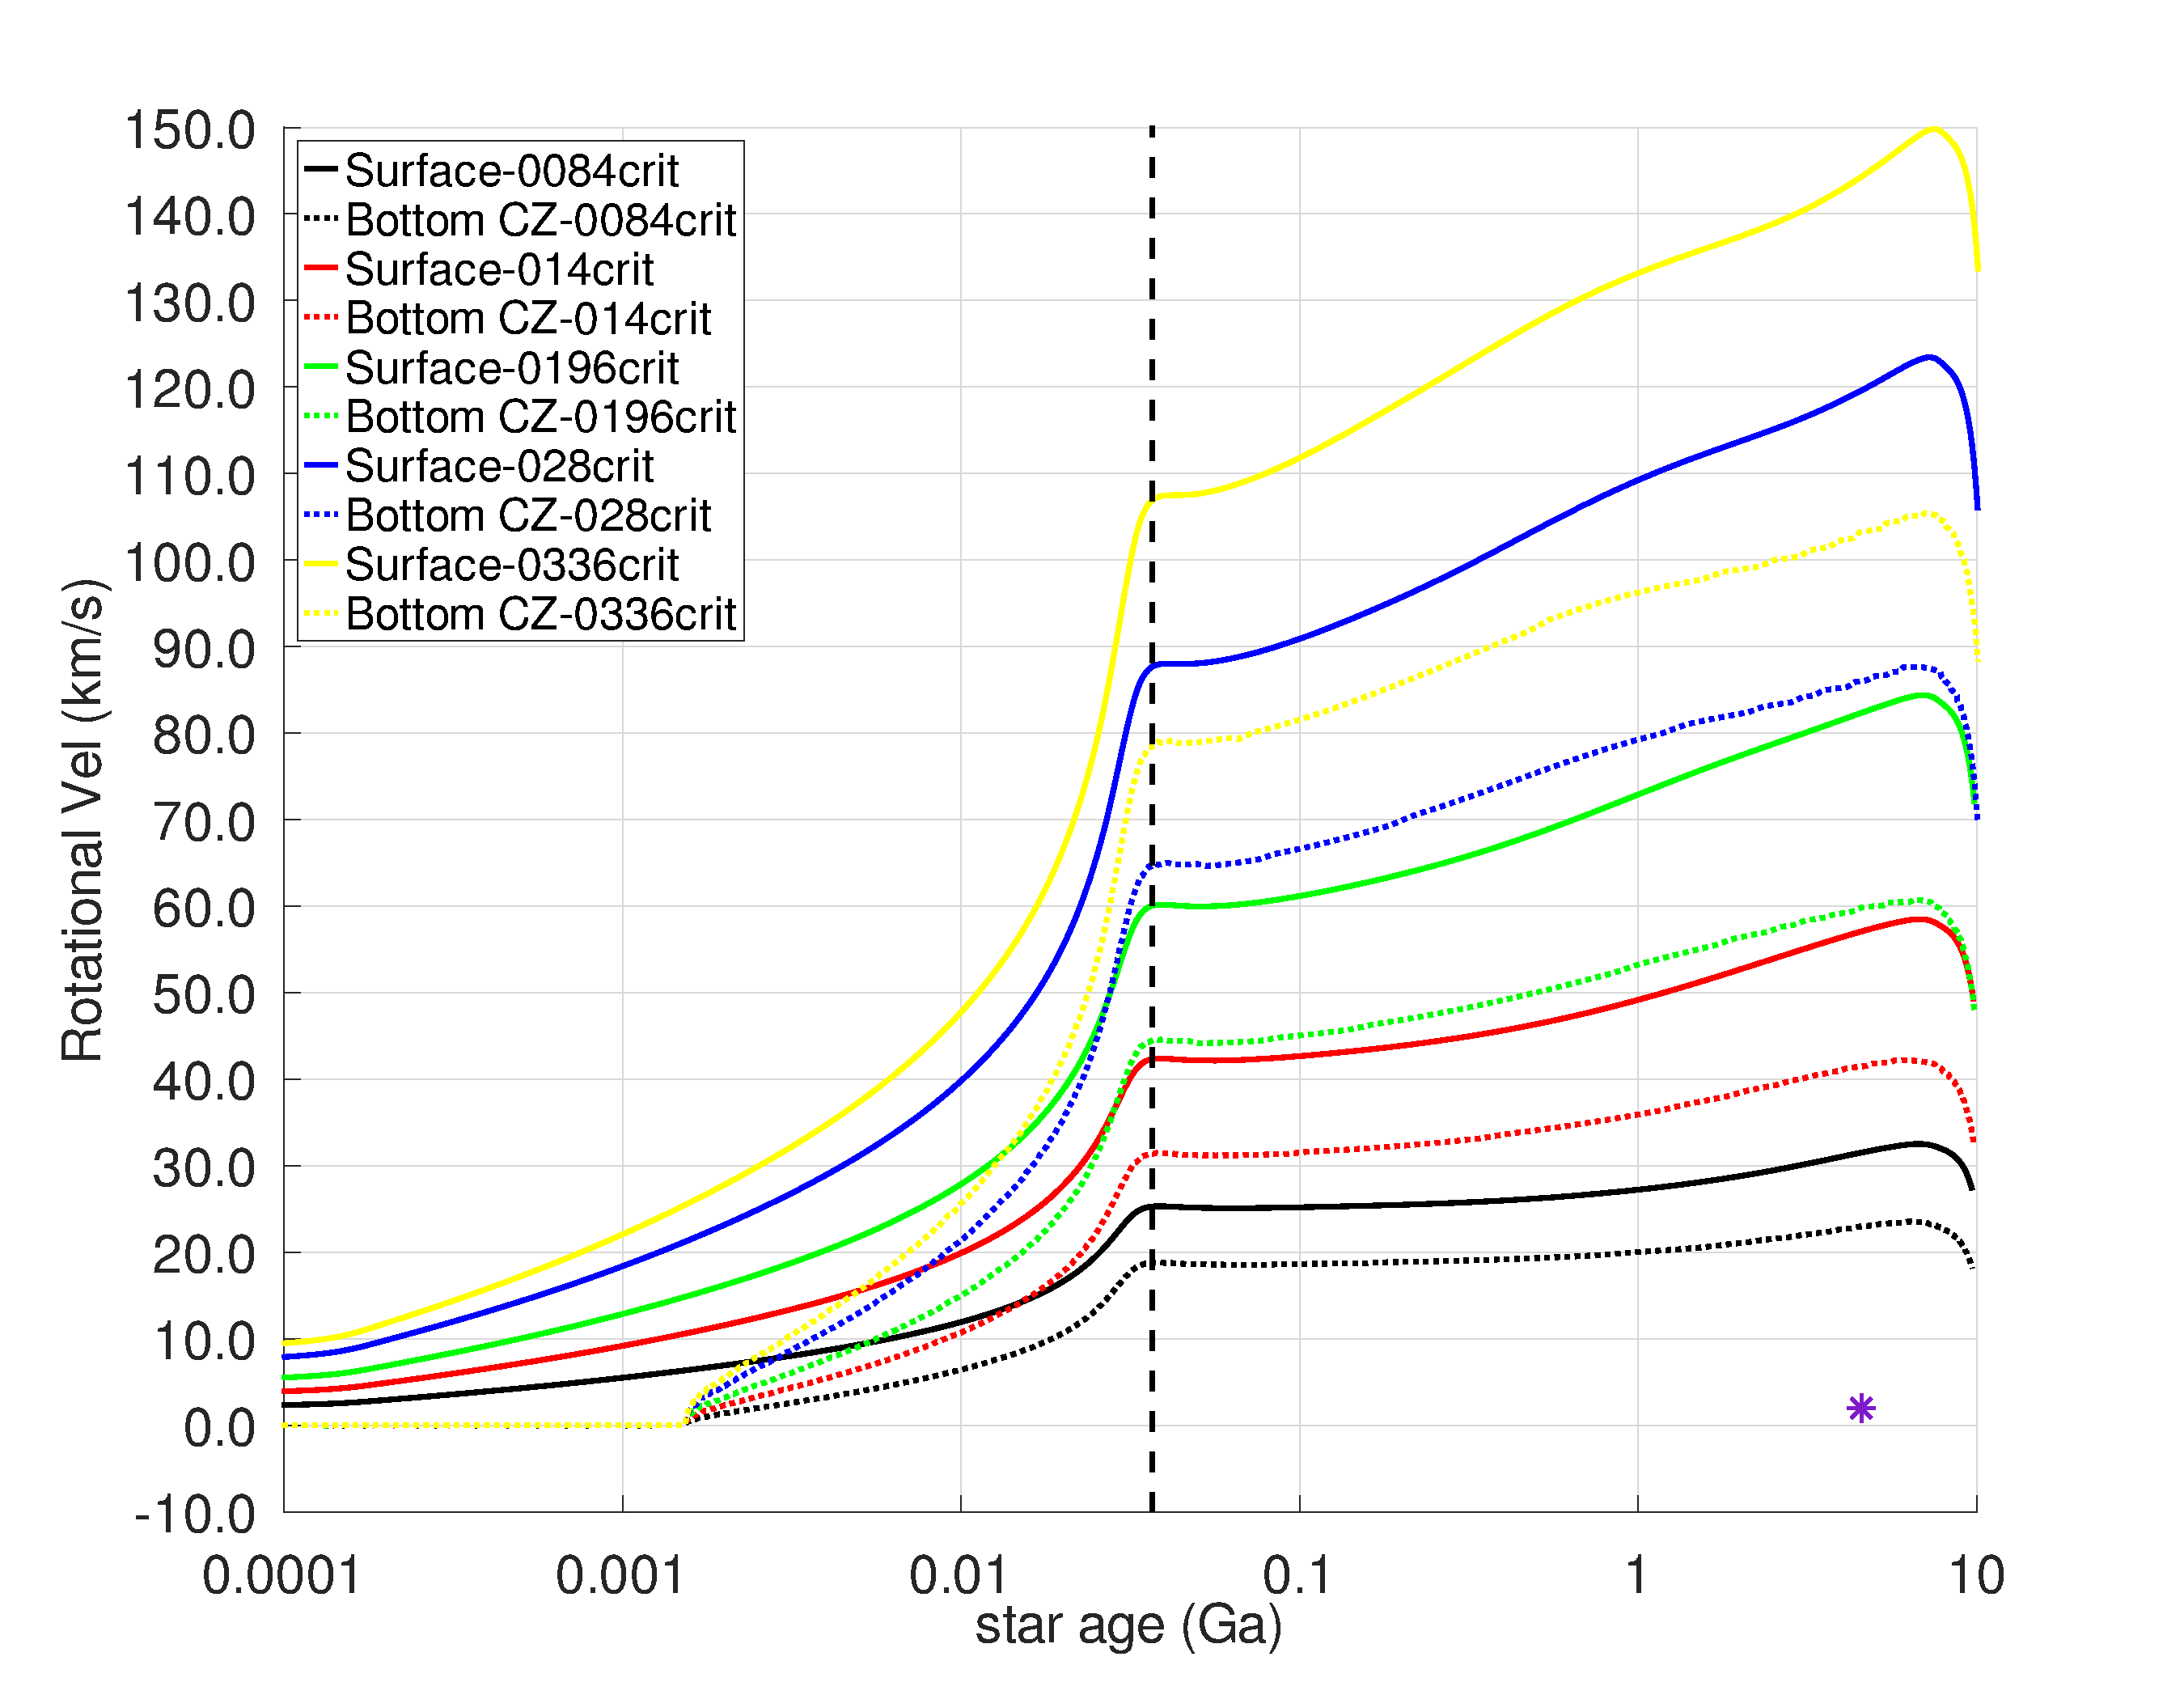
\includegraphics[clip,width=\textwidth]{figures/paper2/rot_vel_var_vel_0_0g_0.pdf}
    \label{fig:subim23}
    \end{subfigure}    
    \begin{subfigure}[h]{0.47\textwidth}
    
\includegraphics[width=\textwidth]{figures/blank.eps}
    \label{fig:subim24}
    \end{subfigure}
\caption{Grid showing the evolution of surface \isotope[7]{Li} abundance relative to \isotope[1]{H}, as a function of time for several 1 $\msun$ models. Each figure shows a set of models in which $\oomegac$ has been fixed and the magnetic field with intensity varies between $0.0\,\Gauss$ and $5.0\,\Gauss$, respectively. The purple star and square are surface Li abundance for the present-day Sun \citep{Asplund2009} and the Pleiades cluster \citep{Sestito2005} respectively. The dashed vertical line makes reference to the ZAMS.}
\label{fig:grid_li_var_g}
\end{figure*}

\begin{figure*}
    \centering
    \begin{subfigure}[h]{0.47\textwidth}
    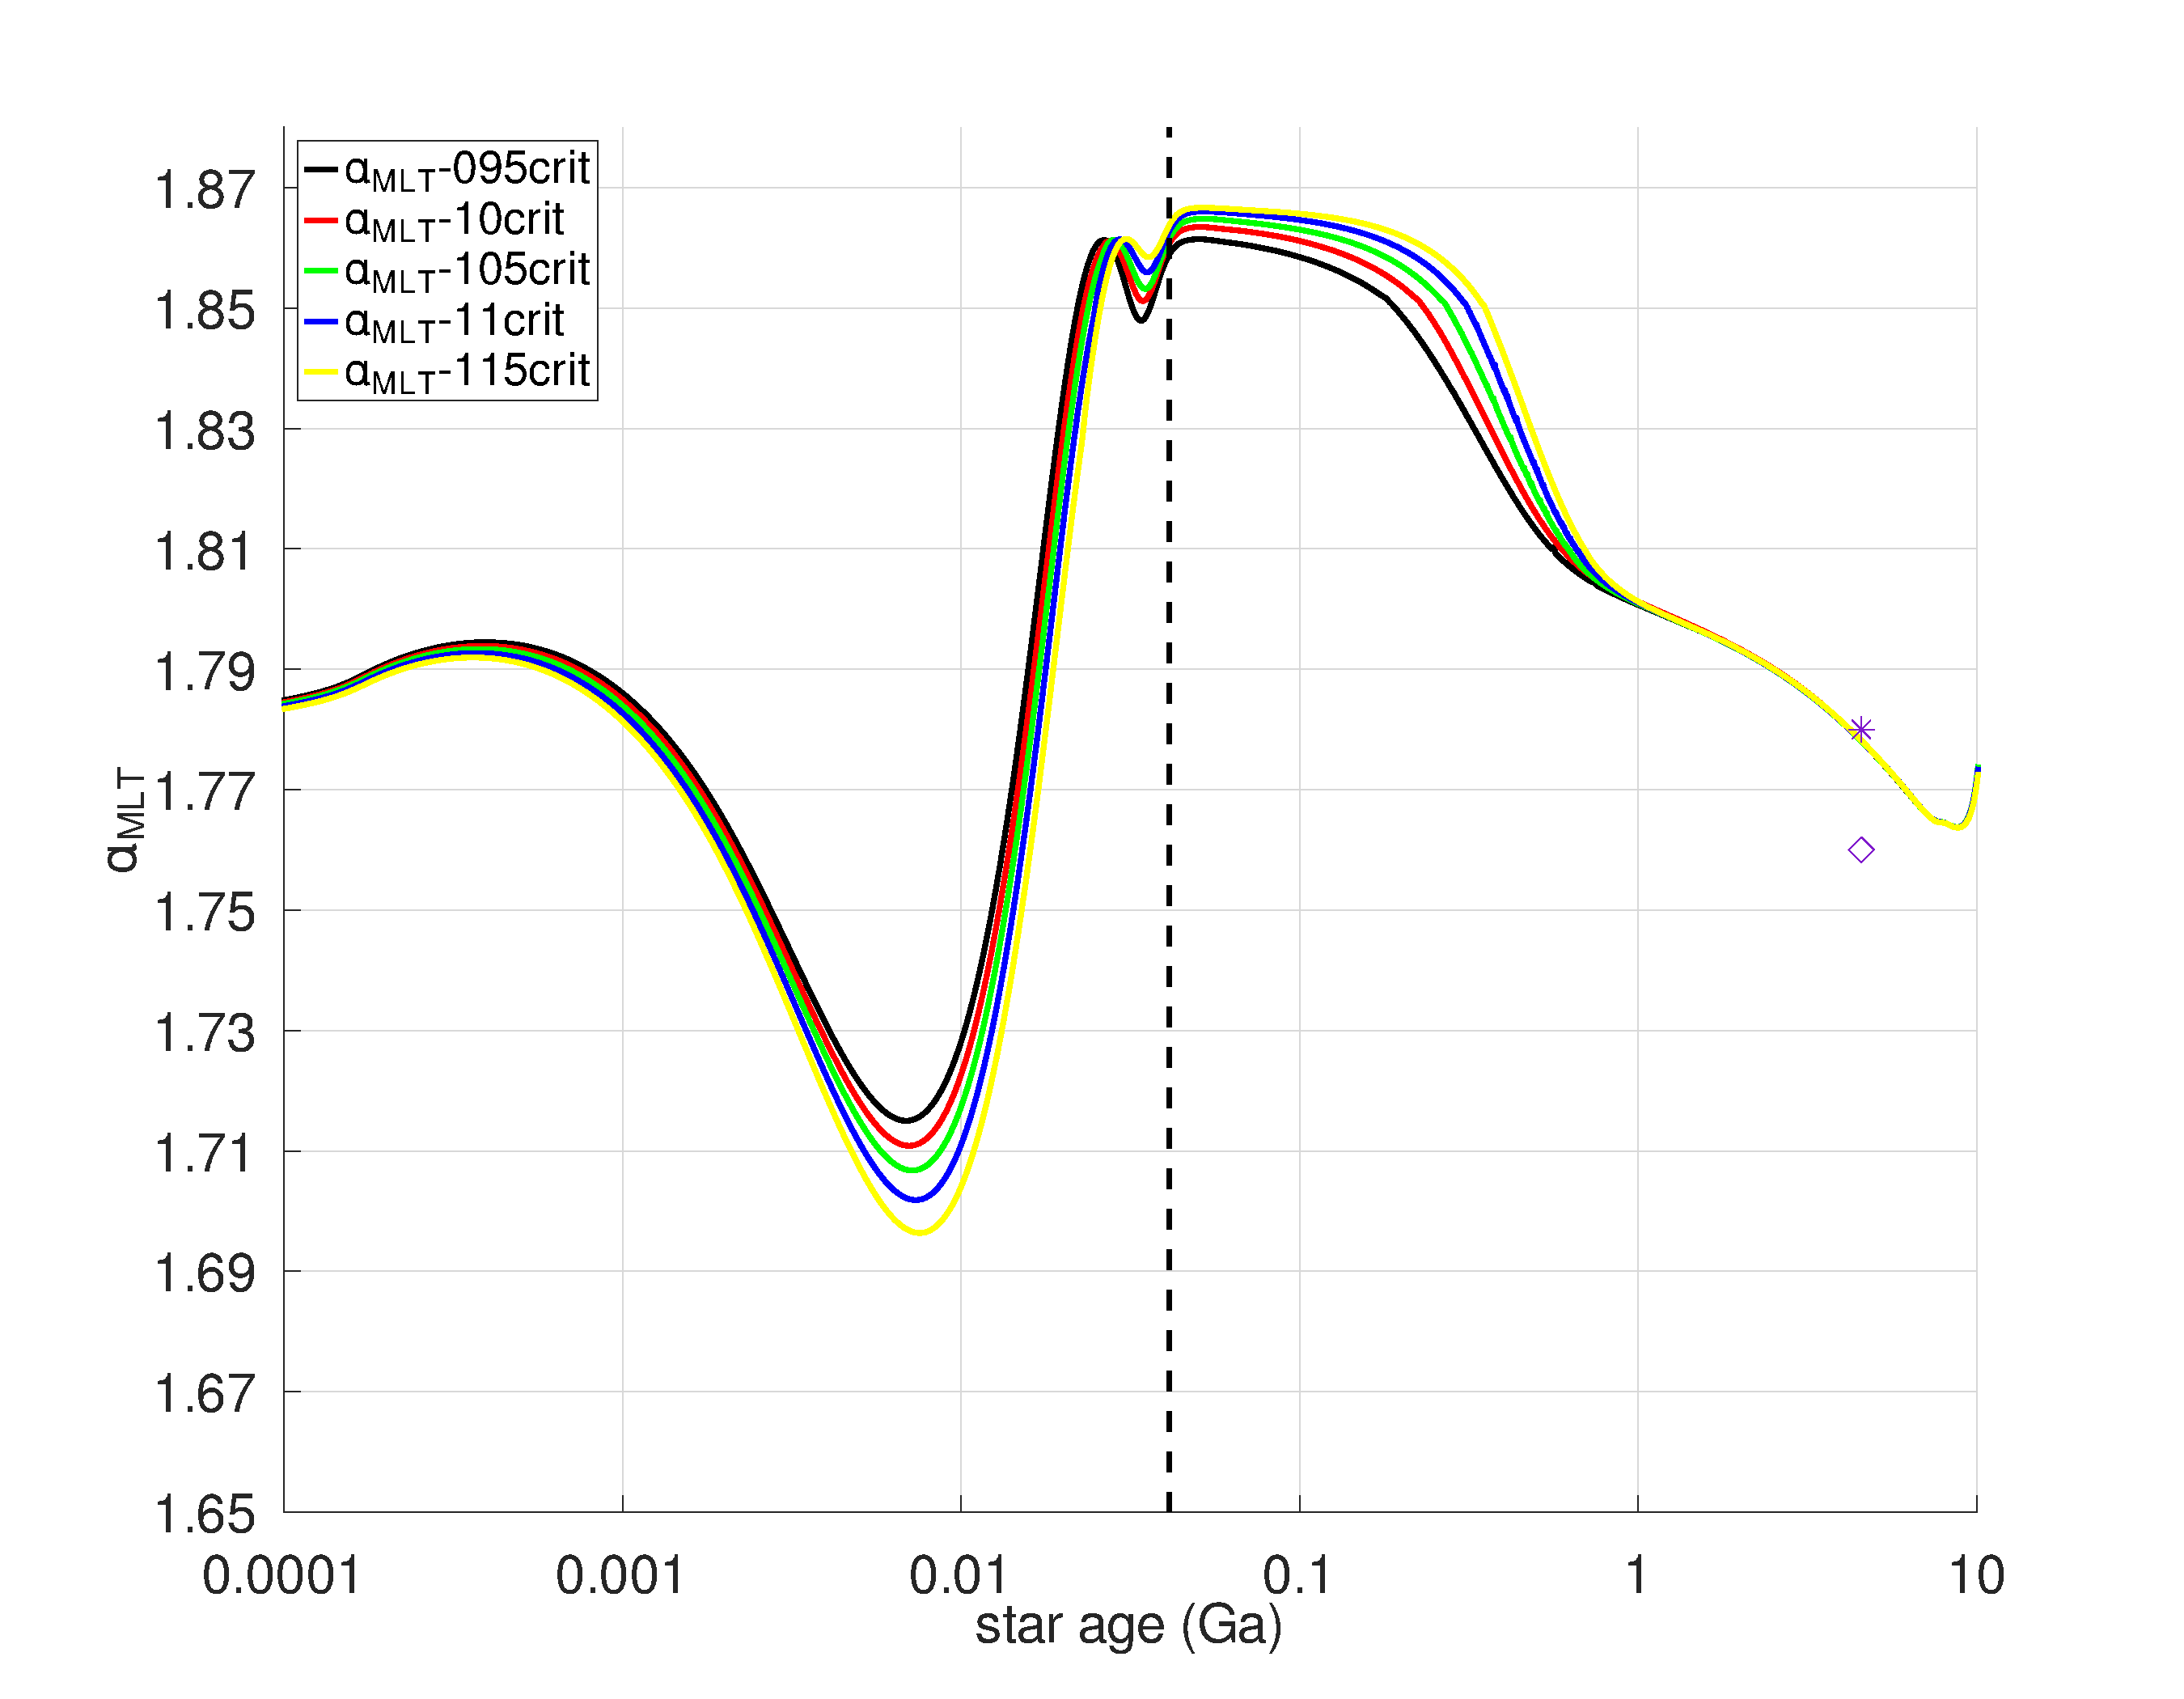
\includegraphics[clip,width=\textwidth]{figures/paper2/alpha_mlt_var_vel_g1.pdf}
    \label{fig:subim41}
    \end{subfigure}
    \begin{subfigure}[h]{0.47\textwidth}
    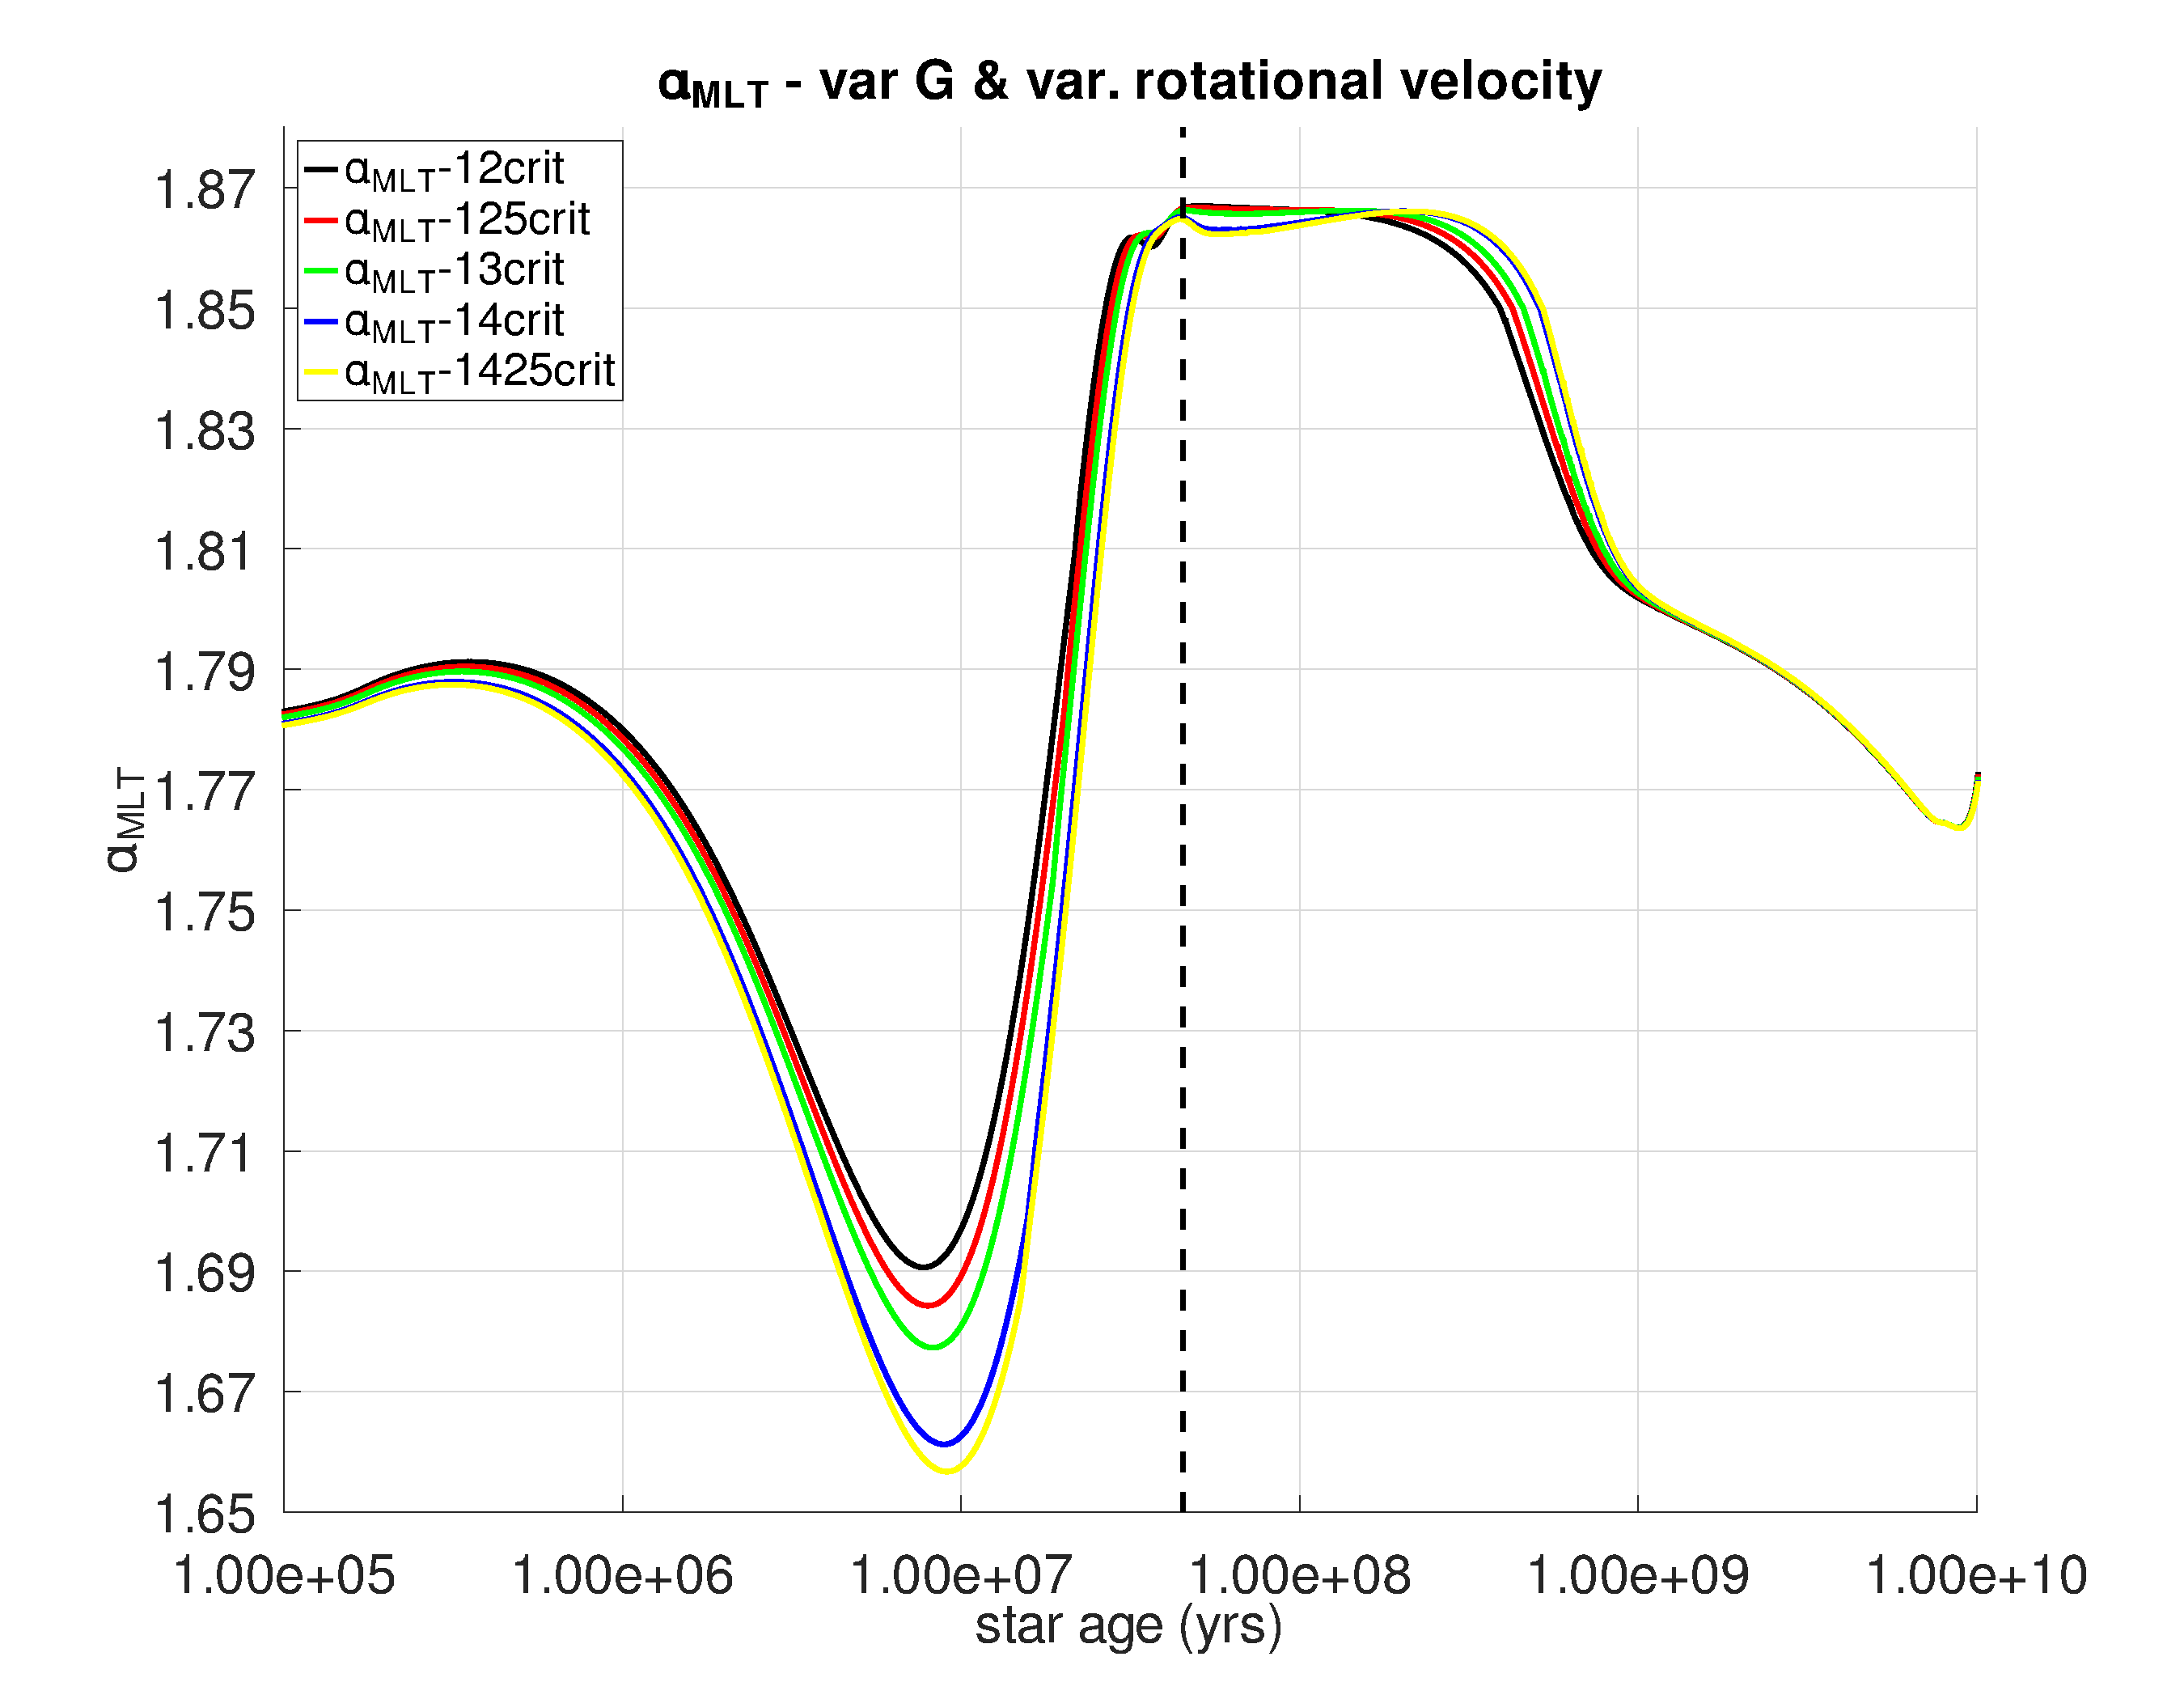
\includegraphics[clip,width=\textwidth]{figures/paper2/alpha_mlt_var_vel_g3.pdf}
    \label{fig:subim42}
    \end{subfigure}
\caption{Grid showing of the evolution of surface rotational velocity, as a function of time for several 1 $\msun$ models. Each figure shows a set of models in which the magnetic field with intensity has been fixed and $\oomegac$ varies between 0.0084 and 0.0336. The purple star is the surface angular velocity for the present-day Sun \citep{Gill2012}. The dashed vertical line makes reference to the ZAMS.}
\label{fig:grid_rot_vel}
\end{figure*}

\appendix
%%%%%%%%%%%%%%%%%%%%%%%%%%%%%%%%%%%%%%%%%%%%%%%%%%



% Don't change these lines
\bsp	% typesetting comment
\label{lastpage}
\end{document}

% End of mnras_template.tex